
%% bare_jrnl_compsoc.tex
%% V1.4b
%% 2015/08/26
%% by Michael Shell
%% See:
%% http://www.michaelshell.org/
%% for current contact information.
%%
%% This is a skeleton file demonstrating the use of IEEEtran.cls
%% (requires IEEEtran.cls version 1.8b or later) with an IEEE
%% Computer Society journal paper.
%%
%% Support sites:
%% http://www.michaelshell.org/tex/ieeetran/
%% http://www.ctan.org/pkg/ieeetran
%% and
%% http://www.ieee.org/

%%*************************************************************************
%% Legal Notice:
%% This code is offered as-is without any warranty either expressed or
%% implied; without even the implied warranty of MERCHANTABILITY or
%% FITNESS FOR A PARTICULAR PURPOSE! 
%% User assumes all risk.
%% In no event shall the IEEE or any contributor to this code be liable for
%% any damages or losses, including, but not limited to, incidental,
%% consequential, or any other damages, resulting from the use or misuse
%% of any information contained here.
%%
%% All comments are the opinions of their respective authors and are not
%% necessarily endorsed by the IEEE.
%%
%% This work is distributed under the LaTeX Project Public License (LPPL)
%% ( http://www.latex-project.org/ ) version 1.3, and may be freely used,
%% distributed and modified. A copy of the LPPL, version 1.3, is included
%% in the base LaTeX documentation of all distributions of LaTeX released
%% 2003/12/01 or later.
%% Retain all contribution notices and credits.
%% ** Modified files should be clearly indicated as such, including  **
%% ** renaming them and changing author support contact information. **
%%*************************************************************************


% *** Authors should verify (and, if needed, correct) their LaTeX system  ***
% *** with the testflow diagnostic prior to trusting their LaTeX platform ***
% *** with production work. The IEEE's font choices and paper sizes can   ***
% *** trigger bugs that do not appear when using other class files.       ***                          ***
% The testflow support page is at:
% http://www.michaelshell.org/tex/testflow/


\documentclass[10pt,journal,compsoc]{IEEEtran}
%
% If IEEEtran.cls has not been installed into the LaTeX system files,
% manually specify the path to it like:
% \documentclass[10pt,journal,compsoc]{../sty/IEEEtran}





% Some very useful LaTeX packages include:
% (uncomment the ones you want to load)


% *** MISC UTILITY PACKAGES ***
%
%\usepackage{ifpdf}
% Heiko Oberdiek's ifpdf.sty is very useful if you need conditional
% compilation based on whether the output is pdf or dvi.
% usage:
% \ifpdf
%   % pdf code
% \else
%   % dvi code
% \fi
% The latest version of ifpdf.sty can be obtained from:
% http://www.ctan.org/pkg/ifpdf
% Also, note that IEEEtran.cls V1.7 and later provides a builtin
% \ifCLASSINFOpdf conditional that works the same way.
% When switching from latex to pdflatex and vice-versa, the compiler may
% have to be run twice to clear warning/error messages.






% *** CITATION PACKAGES ***
%
\ifCLASSOPTIONcompsoc
  % IEEE Computer Society needs nocompress option
  % requires cite.sty v4.0 or later (November 2003)
  \usepackage[nocompress]{cite}
\else
  % normal IEEE
  \usepackage{cite}
\fi
% cite.sty was written by Donald Arseneau
% V1.6 and later of IEEEtran pre-defines the format of the cite.sty package
% \cite{} output to follow that of the IEEE. Loading the cite package will
% result in citation numbers being automatically sorted and properly
% "compressed/ranged". e.g., [1], [9], [2], [7], [5], [6] without using
% cite.sty will become [1], [2], [5]--[7], [9] using cite.sty. cite.sty's
% \cite will automatically add leading space, if needed. Use cite.sty's
% noadjust option (cite.sty V3.8 and later) if you want to turn this off
% such as if a citation ever needs to be enclosed in parenthesis.
% cite.sty is already installed on most LaTeX systems. Be sure and use
% version 5.0 (2009-03-20) and later if using hyperref.sty.
% The latest version can be obtained at:
% http://www.ctan.org/pkg/cite
% The documentation is contained in the cite.sty file itself.
%
% Note that some packages require special options to format as the Computer
% Society requires. In particular, Computer Society  papers do not use
% compressed citation ranges as is done in typical IEEE papers
% (e.g., [1]-[4]). Instead, they list every citation separately in order
% (e.g., [1], [2], [3], [4]). To get the latter we need to load the cite
% package with the nocompress option which is supported by cite.sty v4.0
% and later. Note also the use of a CLASSOPTION conditional provided by
% IEEEtran.cls V1.7 and later.





% *** GRAPHICS RELATED PACKAGES ***
%
\ifCLASSINFOpdf
  % \usepackage[pdftex]{graphicx}
  % declare the path(s) where your graphic files are
  % \graphicspath{{../pdf/}{../jpeg/}}
  % and their extensions so you won't have to specify these with
  % every instance of \includegraphics
  % \DeclareGraphicsExtensions{.pdf,.jpeg,.png}
\else
  % or other class option (dvipsone, dvipdf, if not using dvips). graphicx
  % will default to the driver specified in the system graphics.cfg if no
  % driver is specified.
  % \usepackage[dvips]{graphicx}
  % declare the path(s) where your graphic files are
  % \graphicspath{{../eps/}}
  % and their extensions so you won't have to specify these with
  % every instance of \includegraphics
  % \DeclareGraphicsExtensions{.eps}
\fi
% graphicx was written by David Carlisle and Sebastian Rahtz. It is
% required if you want graphics, photos, etc. graphicx.sty is already
% installed on most LaTeX systems. The latest version and documentation
% can be obtained at: 
% http://www.ctan.org/pkg/graphicx
% Another good source of documentation is "Using Imported Graphics in
% LaTeX2e" by Keith Reckdahl which can be found at:
% http://www.ctan.org/pkg/epslatex
%
% latex, and pdflatex in dvi mode, support graphics in encapsulated
% postscript (.eps) format. pdflatex in pdf mode supports graphics
% in .pdf, .jpeg, .png and .mps (metapost) formats. Users should ensure
% that all non-photo figures use a vector format (.eps, .pdf, .mps) and
% not a bitmapped formats (.jpeg, .png). The IEEE frowns on bitmapped formats
% which can result in "jaggedy"/blurry rendering of lines and letters as
% well as large increases in file sizes.
%
% You can find documentation about the pdfTeX application at:
% http://www.tug.org/applications/pdftex






% *** MATH PACKAGES ***
%
%\usepackage{amsmath}
% A popular package from the American Mathematical Society that provides
% many useful and powerful commands for dealing with mathematics.
%
% Note that the amsmath package sets \interdisplaylinepenalty to 10000
% thus preventing page breaks from occurring within multiline equations. Use:
%\interdisplaylinepenalty=2500
% after loading amsmath to restore such page breaks as IEEEtran.cls normally
% does. amsmath.sty is already installed on most LaTeX systems. The latest
% version and documentation can be obtained at:
% http://www.ctan.org/pkg/amsmath





% *** SPECIALIZED LIST PACKAGES ***
%
%\usepackage{algorithmic}
% algorithmic.sty was written by Peter Williams and Rogerio Brito.
% This package provides an algorithmic environment fo describing algorithms.
% You can use the algorithmic environment in-text or within a figure
% environment to provide for a floating algorithm. Do NOT use the algorithm
% floating environment provided by algorithm.sty (by the same authors) or
% algorithm2e.sty (by Christophe Fiorio) as the IEEE does not use dedicated
% algorithm float types and packages that provide these will not provide
% correct IEEE style captions. The latest version and documentation of
% algorithmic.sty can be obtained at:
% http://www.ctan.org/pkg/algorithms
% Also of interest may be the (relatively newer and more customizable)
% algorithmicx.sty package by Szasz Janos:
% http://www.ctan.org/pkg/algorithmicx




% *** ALIGNMENT PACKAGES ***
%
%\usepackage{array}
% Frank Mittelbach's and David Carlisle's array.sty patches and improves
% the standard LaTeX2e array and tabular environments to provide better
% appearance and additional user controls. As the default LaTeX2e table
% generation code is lacking to the point of almost being broken with
% respect to the quality of the end results, all users are strongly
% advised to use an enhanced (at the very least that provided by array.sty)
% set of table tools. array.sty is already installed on most systems. The
% latest version and documentation can be obtained at:
% http://www.ctan.org/pkg/array


% IEEEtran contains the IEEEeqnarray family of commands that can be used to
% generate multiline equations as well as matrices, tables, etc., of high
% quality.




% *** SUBFIGURE PACKAGES ***
%\ifCLASSOPTIONcompsoc
%  \usepackage[caption=false,font=footnotesize,labelfont=sf,textfont=sf]{subfig}
%\else
%  \usepackage[caption=false,font=footnotesize]{subfig}
%\fi
% subfig.sty, written by Steven Douglas Cochran, is the modern replacement
% for subfigure.sty, the latter of which is no longer maintained and is
% incompatible with some LaTeX packages including fixltx2e. However,
% subfig.sty requires and automatically loads Axel Sommerfeldt's caption.sty
% which will override IEEEtran.cls' handling of captions and this will result
% in non-IEEE style figure/table captions. To prevent this problem, be sure
% and invoke subfig.sty's "caption=false" package option (available since
% subfig.sty version 1.3, 2005/06/28) as this is will preserve IEEEtran.cls
% handling of captions.
% Note that the Computer Society format requires a sans serif font rather
% than the serif font used in traditional IEEE formatting and thus the need
% to invoke different subfig.sty package options depending on whether
% compsoc mode has been enabled.
%
% The latest version and documentation of subfig.sty can be obtained at:
% http://www.ctan.org/pkg/subfig




% *** FLOAT PACKAGES ***
%
%\usepackage{fixltx2e}
% fixltx2e, the successor to the earlier fix2col.sty, was written by
% Frank Mittelbach and David Carlisle. This package corrects a few problems
% in the LaTeX2e kernel, the most notable of which is that in current
% LaTeX2e releases, the ordering of single and double column floats is not
% guaranteed to be preserved. Thus, an unpatched LaTeX2e can allow a
% single column figure to be placed prior to an earlier double column
% figure.
% Be aware that LaTeX2e kernels dated 2015 and later have fixltx2e.sty's
% corrections already built into the system in which case a warning will
% be issued if an attempt is made to load fixltx2e.sty as it is no longer
% needed.
% The latest version and documentation can be found at:
% http://www.ctan.org/pkg/fixltx2e


%\usepackage{stfloats}
% stfloats.sty was written by Sigitas Tolusis. This package gives LaTeX2e
% the ability to do double column floats at the bottom of the page as well
% as the top. (e.g., "\begin{figure*}[!b]" is not normally possible in
% LaTeX2e). It also provides a command:
%\fnbelowfloat
% to enable the placement of footnotes below bottom floats (the standard
% LaTeX2e kernel puts them above bottom floats). This is an invasive package
% which rewrites many portions of the LaTeX2e float routines. It may not work
% with other packages that modify the LaTeX2e float routines. The latest
% version and documentation can be obtained at:
% http://www.ctan.org/pkg/stfloats
% Do not use the stfloats baselinefloat ability as the IEEE does not allow
% \baselineskip to stretch. Authors submitting work to the IEEE should note
% that the IEEE rarely uses double column equations and that authors should try
% to avoid such use. Do not be tempted to use the cuted.sty or midfloat.sty
% packages (also by Sigitas Tolusis) as the IEEE does not format its papers in
% such ways.
% Do not attempt to use stfloats with fixltx2e as they are incompatible.
% Instead, use Morten Hogholm'a dblfloatfix which combines the features
% of both fixltx2e and stfloats:
%
% \usepackage{dblfloatfix}
% The latest version can be found at:
% http://www.ctan.org/pkg/dblfloatfix




%\ifCLASSOPTIONcaptionsoff
%  \usepackage[nomarkers]{endfloat}
% \let\MYoriglatexcaption\caption
% \renewcommand{\caption}[2][\relax]{\MYoriglatexcaption[#2]{#2}}
%\fi
% endfloat.sty was written by James Darrell McCauley, Jeff Goldberg and 
% Axel Sommerfeldt. This package may be useful when used in conjunction with 
% IEEEtran.cls'  captionsoff option. Some IEEE journals/societies require that
% submissions have lists of figures/tables at the end of the paper and that
% figures/tables without any captions are placed on a page by themselves at
% the end of the document. If needed, the draftcls IEEEtran class option or
% \CLASSINPUTbaselinestretch interface can be used to increase the line
% spacing as well. Be sure and use the nomarkers option of endfloat to
% prevent endfloat from "marking" where the figures would have been placed
% in the text. The two hack lines of code above are a slight modification of
% that suggested by in the endfloat docs (section 8.4.1) to ensure that
% the full captions always appear in the list of figures/tables - even if
% the user used the short optional argument of \caption[]{}.
% IEEE papers do not typically make use of \caption[]'s optional argument,
% so this should not be an issue. A similar trick can be used to disable
% captions of packages such as subfig.sty that lack options to turn off
% the subcaptions:
% For subfig.sty:
% \let\MYorigsubfloat\subfloat
% \renewcommand{\subfloat}[2][\relax]{\MYorigsubfloat[]{#2}}
% However, the above trick will not work if both optional arguments of
% the \subfloat command are used. Furthermore, there needs to be a
% description of each subfigure *somewhere* and endfloat does not add
% subfigure captions to its list of figures. Thus, the best approach is to
% avoid the use of subfigure captions (many IEEE journals avoid them anyway)
% and instead reference/explain all the subfigures within the main caption.
% The latest version of endfloat.sty and its documentation can obtained at:
% http://www.ctan.org/pkg/endfloat
%
% The IEEEtran \ifCLASSOPTIONcaptionsoff conditional can also be used
% later in the document, say, to conditionally put the References on a 
% page by themselves.




% *** PDF, URL AND HYPERLINK PACKAGES ***
%
%\usepackage{url}
% url.sty was written by Donald Arseneau. It provides better support for
% handling and breaking URLs. url.sty is already installed on most LaTeX
% systems. The latest version and documentation can be obtained at:
% http://www.ctan.org/pkg/url
% Basically, \url{my_url_here}.





% *** Do not adjust lengths that control margins, column widths, etc. ***
% *** Do not use packages that alter fonts (such as pslatex).         ***
% There should be no need to do such things with IEEEtran.cls V1.6 and later.
% (Unless specifically asked to do so by the journal or conference you plan
% to submit to, of course. )


\usepackage{cite}
\usepackage{amsmath,amssymb,amsfonts, amsthm}
\usepackage{algorithm, algorithmicx}
\usepackage[noend]{algpseudocode}
\usepackage{graphicx}
\usepackage{textcomp}
\usepackage{xcolor}
% Add by author
\usepackage{cite}
\usepackage{amsmath}
\usepackage{booktabs}
\usepackage{url}
% \usepackage{fontspec}

% correct bad hyphenation here
\hyphenation{op-tical net-works semi-conduc-tor}

% Defined by authors--------------------------------------------
\newtheorem{problem}{Problem}
\newtheorem{lemma}{Lemma}
\newtheorem{theorem}{Theorem}
\newcommand{\Bo}[1]{{\color{red} Bo: #1}}
% \newcommand{\QM}[1]{{\color{blue} QM: #1}}
\newcommand{\QM}[1]{{\color{blue}{#1}}}

\newcommand{\D}{\mathcal{T}}
\newcommand{\V}{\mathsf{V}}
\newcommand{\oR}{\mathcal{R}}
\newcommand{\VV}{\mathtt{V}}
\newcommand{\QQ}{\mathtt{Q}}
\newcommand{\MU}{\mathsf{U}}
\newcommand{\vats}{\mathsf{VQGS}}
\newcommand{\vatss}{\mathsf{VQGS}^+}
\newcommand{\vatssce}{\mathsf{VQGS}^+\mathsf{CE}}
\newcommand{\rand}{\mathsf{Random}}
\newcommand{\full}{\mathsf{Full}}
\newcommand{\avats}{\mathsf{CheetahTraj}}
\newcommand{\cavats}{\mathsf{CheetahTraj}\mathsf{CE}}
\newcommand{\qtavats}{\mathsf{CheetahTraj}-\mathsf{QT}}
\newcommand{\sz}{\textsf{Shenzhen}}
\newcommand{\pt}{\textsf{Porto}}
\newcommand{\cd}{\textsf{Chengdu}}
\newcommand{\prob}{\textsf{QOSP}}
\newcommand{\query}{\mathcal{Q}}
\newcommand{\wpts}{\mathsf{WayPoint}}
\newcommand{\invQ}{\mathsf{InvQuad}}
\newcommand{\II}{\mathcal{I}}

\newcommand{\trim}{\vspace{-2mm}}

\newcommand{\baseline}{\mathsf{baseline}}

\newcommand{\stitle}[1]{\vspace*{0.4em}\noindent{\bf #1:\/}}
\newcommand{\sstitle}[1]{\vspace*{0.4em}\noindent{\bf #1\/.}}


\newcommand{\localavats}{\mathsf{local+fix}}

\newcommand{\squishlist}{
	\begin{list}{$\bullet$}
		{ \setlength{\itemsep}{0pt}
			\setlength{\parsep}{3pt}
			\setlength{\topsep}{3pt}
			\setlength{\partopsep}{0pt}
			\setlength{\leftmargin}{1.2em}
			\setlength{\labelwidth}{1em}
			\setlength{\labelsep}{0.6em}
		}
	}
	\newcommand{\squishend}{
	\end{list}
}



\begin{document}
%
% paper title
% Titles are generally capitalized except for words such as a, an, and, as,
% at, but, by, for, in, nor, of, on, or, the, to and up, which are usually
% not capitalized unless they are the first or last word of the title.
% Linebreaks \\ can be used within to get better formatting as desired.
% Do not put math or special symbols in the title.
\title{$\avats$: Quality and Efficiency in Large-scale Trajectory Data Visual Exploration}
%
%
% author names and IEEE memberships
% note positions of commas and nonbreaking spaces ( ~ ) LaTeX will not break
% a structure at a ~ so this keeps an author's name from being broken across
% two lines.
% use \thanks{} to gain access to the first footnote area
% a separate \thanks must be used for each paragraph as LaTeX2e's \thanks
% was not built to handle multiple paragraphs
%
%
%\IEEEcompsocitemizethanks is a special \thanks that produces the bulleted
% lists the Computer Society journals use for "first footnote" author
% affiliations. Use \IEEEcompsocthanksitem which works much like \item
% for each affiliation group. When not in compsoc mode,
% \IEEEcompsocitemizethanks becomes like \thanks and
% \IEEEcompsocthanksitem becomes a line break with idention. This
% facilitates dual compilation, although admittedly the differences in the
% desired content of \author between the different types of papers makes a
% one-size-fits-all approach a daunting prospect. For instance, compsoc 
% journal papers have the author affiliations above the "Manuscript
% received ..."  text while in non-compsoc journals this is reversed. Sigh.
\author{Qiaomu Shen,
	Chaozu Zhang,
	Xiao Yan,
	Chuan Yang,
	Dan Zeng,
	Wei Zeng,
	Bo Tang
% <-this % stops an unwanted space
%	\thanks{Manuscript received April 19, 2005; revised August 26, 2015.}
}

\if 0
\author{Michael~Shell,~\IEEEmembership{Member,~IEEE,}
        John~Doe,~\IEEEmembership{Fellow,~OSA,}
        and~Jane~Doe,~\IEEEmembership{Life~Fellow,~IEEE}% <-this % stops a space
\IEEEcompsocitemizethanks{\IEEEcompsocthanksitem M. Shell was with the Department
of Electrical and Computer Engineering, Georgia Institute of Technology, Atlanta,
GA, 30332.\protect\\
% note need leading \protect in front of \\ to get a newline within \thanks as
% \\ is fragile and will error, could use \hfil\break instead.
E-mail: see http://www.michaelshell.org/contact.html
\IEEEcompsocthanksitem J. Doe and J. Doe are with Anonymous University.}% <-this % stops an unwanted space
\thanks{Manuscript received April 19, 2005; revised August 26, 2015.}}
\fi
% note the % following the last \IEEEmembership and also \thanks - 
% these prevent an unwanted space from occurring between the last author name
% and the end of the author line. i.e., if you had this:
% 
% \author{....lastname \thanks{...} \thanks{...} }
%                     ^------------^------------^----Do not want these spaces!
%
% a space would be appended to the last name and could cause every name on that
% line to be shifted left slightly. This is one of those "LaTeX things". For
% instance, "\textbf{A} \textbf{B}" will typeset as "A B" not "AB". To get
% "AB" then you have to do: "\textbf{A}\textbf{B}"
% \thanks is no different in this regard, so shield the last } of each \thanks
% that ends a line with a % and do not let a space in before the next \thanks.
% Spaces after \IEEEmembership other than the last one are OK (and needed) as
% you are supposed to have spaces between the names. For what it is worth,
% this is a minor point as most people would not even notice if the said evil
% space somehow managed to creep in.



% The paper headers
\markboth{Journal of \LaTeX\ Class Files,~Vol.~14, No.~8, August~2015}%
{Shell \MakeLowercase{\textit{et al.}}: Bare Demo of IEEEtran.cls for Computer Society Journals}
% The only time the second header will appear is for the odd numbered pages
% after the title page when using the twoside option.
% 
% *** Note that you probably will NOT want to include the author's ***
% *** name in the headers of peer review papers.                   ***
% You can use \ifCLASSOPTIONpeerreview for conditional compilation here if
% you desire.



% The publisher's ID mark at the bottom of the page is less important with
% Computer Society journal papers as those publications place the marks
% outside of the main text columns and, therefore, unlike regular IEEE
% journals, the available text space is not reduced by their presence.
% If you want to put a publisher's ID mark on the page you can do it like
% this:
%\IEEEpubid{0000--0000/00\$00.00~\copyright~2015 IEEE}
% or like this to get the Computer Society new two part style.
%\IEEEpubid{\makebox[\columnwidth]{\hfill 0000--0000/00/\$00.00~\copyright~2015 IEEE}%
%\hspace{\columnsep}\makebox[\columnwidth]{Published by the IEEE Computer Society\hfill}}
% Remember, if you use this you must call \IEEEpubidadjcol in the second
% column for its text to clear the IEEEpubid mark (Computer Society jorunal
% papers don't need this extra clearance.)



% use for special paper notices
%\IEEEspecialpapernotice{(Invited Paper)}



% for Computer Society papers, we must declare the abstract and index terms
% PRIOR to the title within the \IEEEtitleabstractindextext IEEEtran
% command as these need to go into the title area created by \maketitle.
% As a general rule, do not put math, special symbols or citations
% in the abstract or keywords.
\IEEEtitleabstractindextext{%
\begin{abstract}
Visualizing large-scale trajectory data is a core subroutine for many applications, e.g., traffic management, urban planning, and route recommendation.
However, naively visualizing all trajectories for a target region could result in long delay due to large data volume.
Ad-hoc sampling can reduce visualization time but may harm visual quality, i.e., generating visualizations that look substantially different from the exact one.
In this paper, we propose the $\avats$ framework to provide high quality trajectory visualization for arbitrary target region with low latency.
To this end, we first define a natural pixel-based \textit{visual quality function} to measure the similarity between two visualizations and formulate a quality optimal trajectory sampling problem.
Then, we design the $\vats$ and $\vatss$ algorithms to solve the trajectory sampling problem, which not only provide guaranteed visual quality but also reduce visual clutter.
To generate quality guaranteed trajectory samples with high efficiency, we develop quad-tree-based index ($\invQ$) that allows to use trajectory samples computed offline.
Extensive experiments (i.e., case-, user-, and quantitative- studies) are conducted on 3 real-world trajectory datasets to verify visualization quality and efficiency of $\avats$. The results show that $\avats$ consistently provide high quality visualizations and its visualization time is orders of magnitude shorter than visualizing all trajectories.   	
%Visualizing large-scale trajectory data is a core subroutine for many smart city applications, e.g., traffic management, urban planning, and route recommendation. The task is challenging due to high scalability requirement and severe visual clutter. Sampling can effectively mitigate both problems but may harm visual fidelity, i.e., generating visualizations that look different from the exact one. In this work, we propose sampling techniques that provide \textit{theoretically guaranteed visual fidelity} for large-scale trajectory data visualization. We first define a natural pixel-based \textit{fidelity loss function} to measure the difference between two visualizations. However, our analysis shows that it is NP-hard to sample a fixed-size subset of trajectories to minimize the loss function. Therefore, we then devise an approximate algorithm named \textit{$\vats$} with a suite of optimization techniques, which runs efficiently but still provides guaranteed fidelity loss. By taking data distribution and human perception characteristics into consideration, we further improve $\vats$ to an advanced algorithm named $\avats$ to tackle the visual clutter problem. Extensive experiments (i.e., case-, user-, and quantitative- studies) are also conducted on real-world trajectory datasets to verify the effectiveness and efficiency of our proposals.
%In addition, comprehensive user studies further illustrate the superiority of our proposals in various applications, e.g., traffic flow comparison, and reachable route inspection.
\end{abstract}

% Note that keywords are not normally used for peerreview papers.
\begin{IEEEkeywords}
Trajectory visualization, interactive data exploration, sampling
\end{IEEEkeywords}}


% make the title area
\maketitle


% To allow for easy dual compilation without having to reenter the
% abstract/keywords data, the \IEEEtitleabstractindextext text will
% not be used in maketitle, but will appear (i.e., to be "transported")
% here as \IEEEdisplaynontitleabstractindextext when the compsoc 
% or transmag modes are not selected <OR> if conference mode is selected 
% - because all conference papers position the abstract like regular
% papers do.
\IEEEdisplaynontitleabstractindextext
% \IEEEdisplaynontitleabstractindextext has no effect when using
% compsoc or transmag under a non-conference mode.



% For peer review papers, you can put extra information on the cover
% page as needed:
% \ifCLASSOPTIONpeerreview
% \begin{center} \bfseries EDICS Category: 3-BBND \end{center}
% \fi
%
% For peerreview papers, this IEEEtran command inserts a page break and
% creates the second title. It will be ignored for other modes.
\IEEEpeerreviewmaketitle

\IEEEraisesectionheading{\section{Introduction}\label{sec:intro}}
The ubiquity of location-acquisition devices leads to an explosive growth of movement data (i.e., trajectories), e.g., for vehicles, shared bikes and pedestrians. Visualizing these large-scale trajectory data is crucial for many smart city applications~\cite{wang2014visual,tang2017efficient,zheng2011learning} and location-based services~\cite{liu2016smartadp, zheng2010collaborative}. Among various visualization methods, line-based trajectory visualization, which connects the locations of a moving object by polylines, is widely adopted for spatial-temporal data analytics~\cite{chen2015survey,visualanalysis,bigchanvis}. To support interactive exploration on trajectory data, it is crucial to conduct  line-based trajectory visualization for an arbitrary target region with high quality and low latency.






%VLDB
%Nowadays, the ubiquity of location-acquisition devices leads to an explosive growth of the volume of movement data (i.e., trajectories), e.g., for vehicles, shared bikes and pedestrians. Visualizing these large-scale trajectory data is crucial for many smart city applications~\cite{wang2014visual,tang2017efficient,zheng2011learning} and location-based services~\cite{liu2016smartadp, zheng2010collaborative}. Among various visualization methods, line-based trajectory visualization, which connects the locations of a moving object by polylines, is widely adopted for spatial-temporal data analytics~\cite{chen2015survey,visualanalysis,bigchanvis}. However, large-scale line-based trajectory visualization suffers from two problems--(i) \textit{scalability} and (ii) \textit{visual clutter}, which we elaborate as follows.

%\textit{visual clutter}~\cite{kwon2017sampling}.




\stitle{Long visualization time for large-scale datasets} To visualize the trajectories in a target region $\query$, a natural solution is to find the trajectories in it and visualize all these trajectories ($\full$ for short). However, $\full$ may suffer from a long visualization time as the trajectory datasets can be extremely large. For example, Shenzhen has 24,237 taxis which collectively generate more than 7.72 million GPS locations each day~\cite{sz}. In addition, our profiling results in Table~\ref{tab:gpu}\footnote{Mapping is the time to map the GPS points to the screen points, and rendering is the time to render the screen points. The settings of this measurement can be found in Section~\ref{sec:exp}.} show that it takes 16.154 seconds to visualize the 1,000,000 taxi trajectories in the \pt{} dataset. As visualization time scales almost linearly with the number of trajectories (see Table~\ref{tab:gpu}), $\full$ could take a long time if there are many trajectories in the target region. However, interactive visual exploration typically requires the visualization to be generated in less than 1 second~\cite{shneiderman1984response}. Another problem of applying $\full$ on large-scale datasets is~\textit{visual clutter}~\cite{kwon2017sampling}, where there are too many points in the visualization such that it is difficult for human users to gain insights. We provide an example Figure~\ref{fig:overview}(A) for the \pt{} dataset, for which it is almost impossible to recognize the road networks in the dense region at the center.

\begin{table}
	\centering
	\small
	\caption{Visualization time on the \pt{} dataset (in seconds)}
    \trim
	\begin{tabular}{|c|c|c|c|c|} \hline
		No. of  & No. of & Mapping & Rendering & Total \\
         trajectories &  GPS points & time & time & time \\ \hline
		1,000& 31,300 & 0.027 & 0.003 & 0.03 \\ \hline
		10,000& 31,6531 & 0.169 & 0.005 & 0.174\\ \hline
		100,000& 316,7120 & 1.701 & 0.057 & 1.758 \\ \hline
		1,000,000& 31,646,379 & 15.562 & 0.592 & 16.154 \\ \hline
	\end{tabular}	\label{tab:gpu}
    \trim \trim 
\end{table}


%\stitle{Visual clutter} It is a common problem for large-scale data visualization, which we illustrate with an example in Figure~\ref{fig:overview}(A). Because of visual clutter, it is almost impossible to recognize the road network in the embedded figure of Figure~\ref{fig:overview}(A), making it difficult for human-users to gain insights from the visualization. Hence, we want the trajectory visualization to be visual-clutter-free for good user experience.

%VLDB
%\stitle{Scalability}
%Trajectory datasets can be extremely large and thus take a long time to render for visualization. For example, Shenzhen has 24,237 taxis which collectively generate more than 82.8 million GPS locations each day~\cite{sz}. Our benchmark on the \pt{} taxi trajectory dataset shows that it takes 13.95 seconds to render 1 million real-world trajectories using an NVIDIA GeForce GTX 1080 GPU with 8GB video memory. The long delay caused by large dataset cardinality makes interactive visual exploration difficult. Thus, we want visualization to scale to very large datasets while maintaining a short delay.


%In New York, {there are} over 13,000 taxis carrying over 1 million passengers and making 500,000 trips on an average day~\cite{ferreira2013visual}.

%Rendering refers to the use of the hardware device (e.g., GPU) in the generation of visualizations.

%However, the rendering capability of modern commodity GPUs is limited.
%We did a benchmark experiment to evaluate the rendering capability of NVIDIA GeForce GTX 1080 with 8GB video memory.
%It needs 13.95 seconds to render 1 million real-world trajectories in \pt{}. % with 32.66 millions GPS points.
%Obviously, it cannot support interactive visual exploration in large-scale trajectory dataset.
%Thus, how to support scalable visualization is the first challenge in large trajectory data visualization problem.



%It is almost impossible to
%
%It is a common issue in big data visualization~\cite{clutter}.
%Figure~\ref{fig:teaser}(A) is the visualization result of the full \pt{} taxi trajectory dataset.
%Intuitively, the region shown in the embedded figure of A suffers visual clutter issue seriously,
%i.e., the road network almost cannot be recognized in it,
%which hinders the abilities of human-users to explore the dataset and identify the underlying data insights.
%Hence, the second challenge in large trajectory data visualization problem is how to address visual clutter issue.



%To overcome the above challenges, several visualization approaches have been proposed in the literature.
%Unfortunately, none of them could address these three challenges simultaneously and perfectly.
%In particular, the spatial aggregation based approaches~\cite{zeng2013visualizing,von2015mobilitygraphs} preprocess the massive movement data, and visualize the results after preprocessing.
%The aggregation based methods ignored the visual clutter in raw spatial data as they only visualize the aggregated/preprocessed results.
%In other words, their visualization results may lose the detail information in raw data.
%%These approaches alleviate the large data size and limited rendering ability issues in large-scale spatial data visualization.
%%Nevertheless, they ignored the visual clutter issue in raw spatial data as they only visualize the aggregated/preprocessed results.
%In recent years, many visualization research works are proposed to address visual clutter,
%e.g., edge bundling~\cite{zeng2019route, thony2015vector} and density map~\cite{lampe2011interactive, scheepens2011interactive}.
%However, these works neither focus on line-based trajectory visualization nor designed for large-scale trajectory dataset.

% \begin{figure*}[t]
% 	\centering
% 	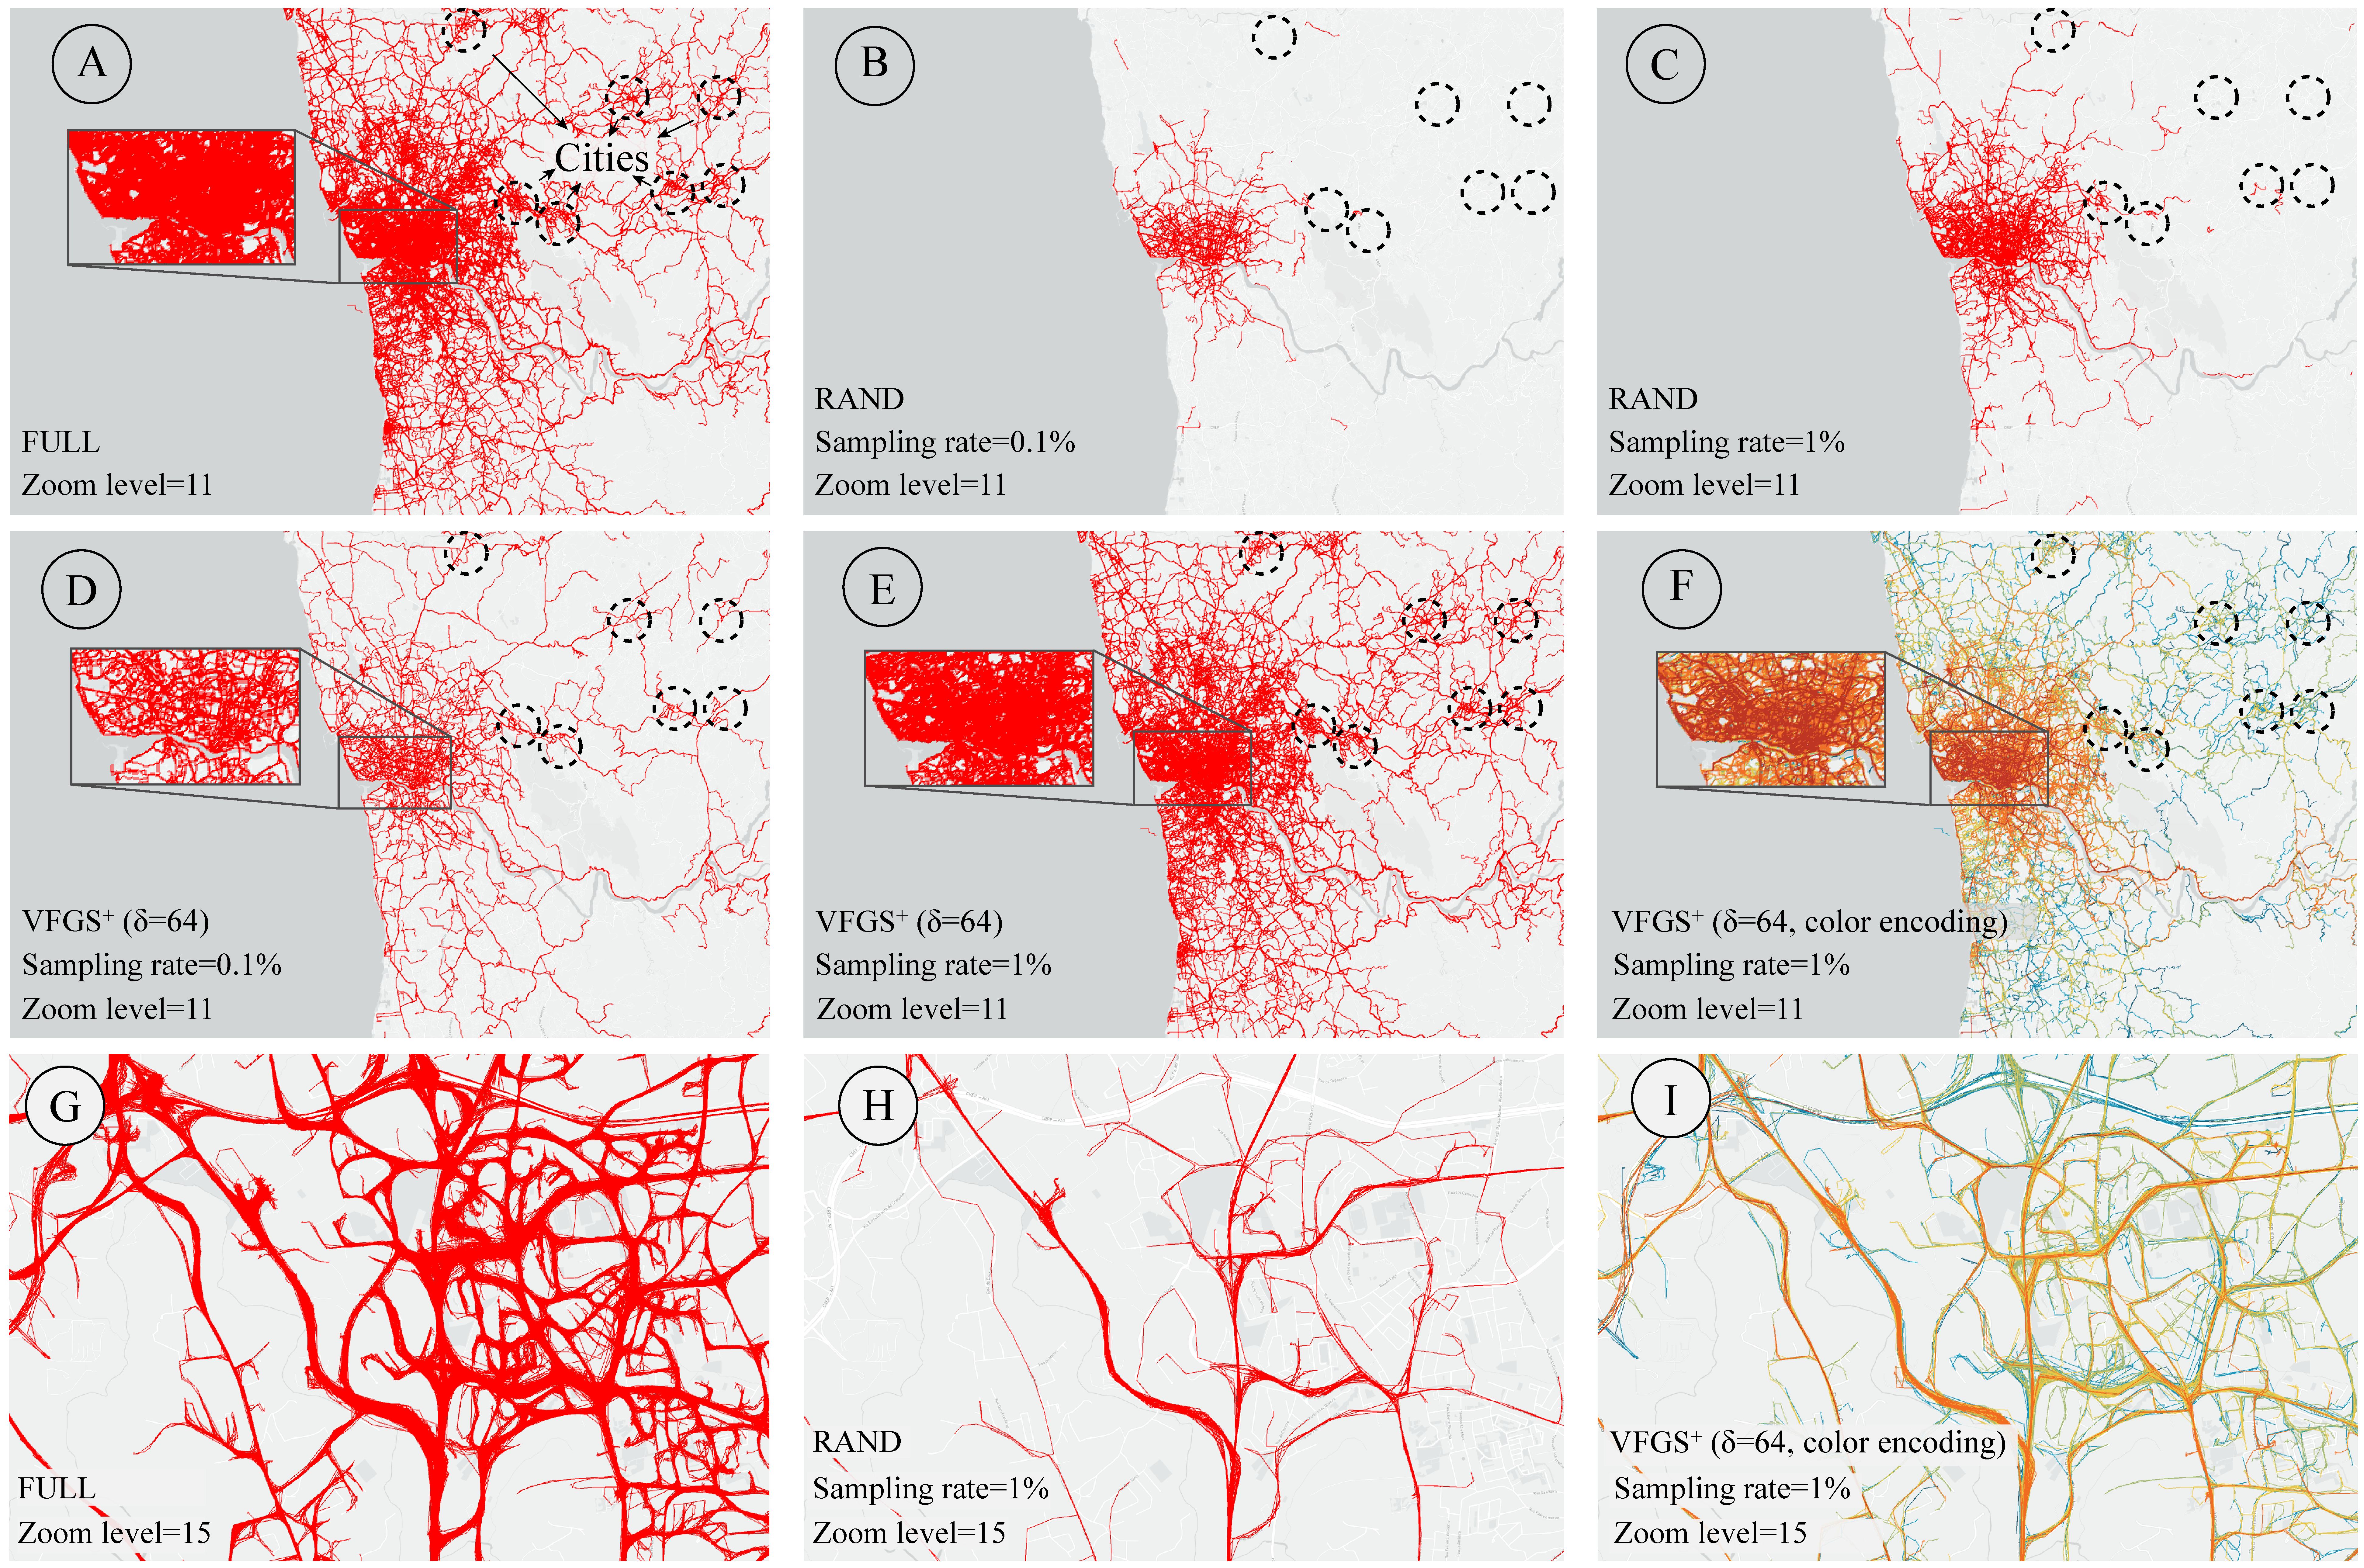
\includegraphics[width=0.90\textwidth]{pictures/Teaser.pdf}
% 	\vspace{-2mm}
% 	\caption{A comparison of visualization results. (I) A is the visualization of the full \pt{} taxi trajectory dataset at zoom level 11.
%     At the same zoom level, B and C are produced by uniform random sampling,
%     while D, E, F are produced by our $\avats$ algorithm.
%     (II) G is the visualization of the full \pt{} dataset at zoom level 15, while H and I are the corresponding results of uniform random sampling and $\avats$, respectively.
%     (III) F and I are generated by $\avats$ with color encoding for representativeness to combat visual clutter.
%     Best viewed in color.}
% 	\label{fig:teaser}
% \trim \trim
% \end{figure*}

% \QM{Introduce the data to visualization time: database/file - memory - data transformation(GPS to screen position)- visualization}.

\begin{figure*}[t]
	\centering
	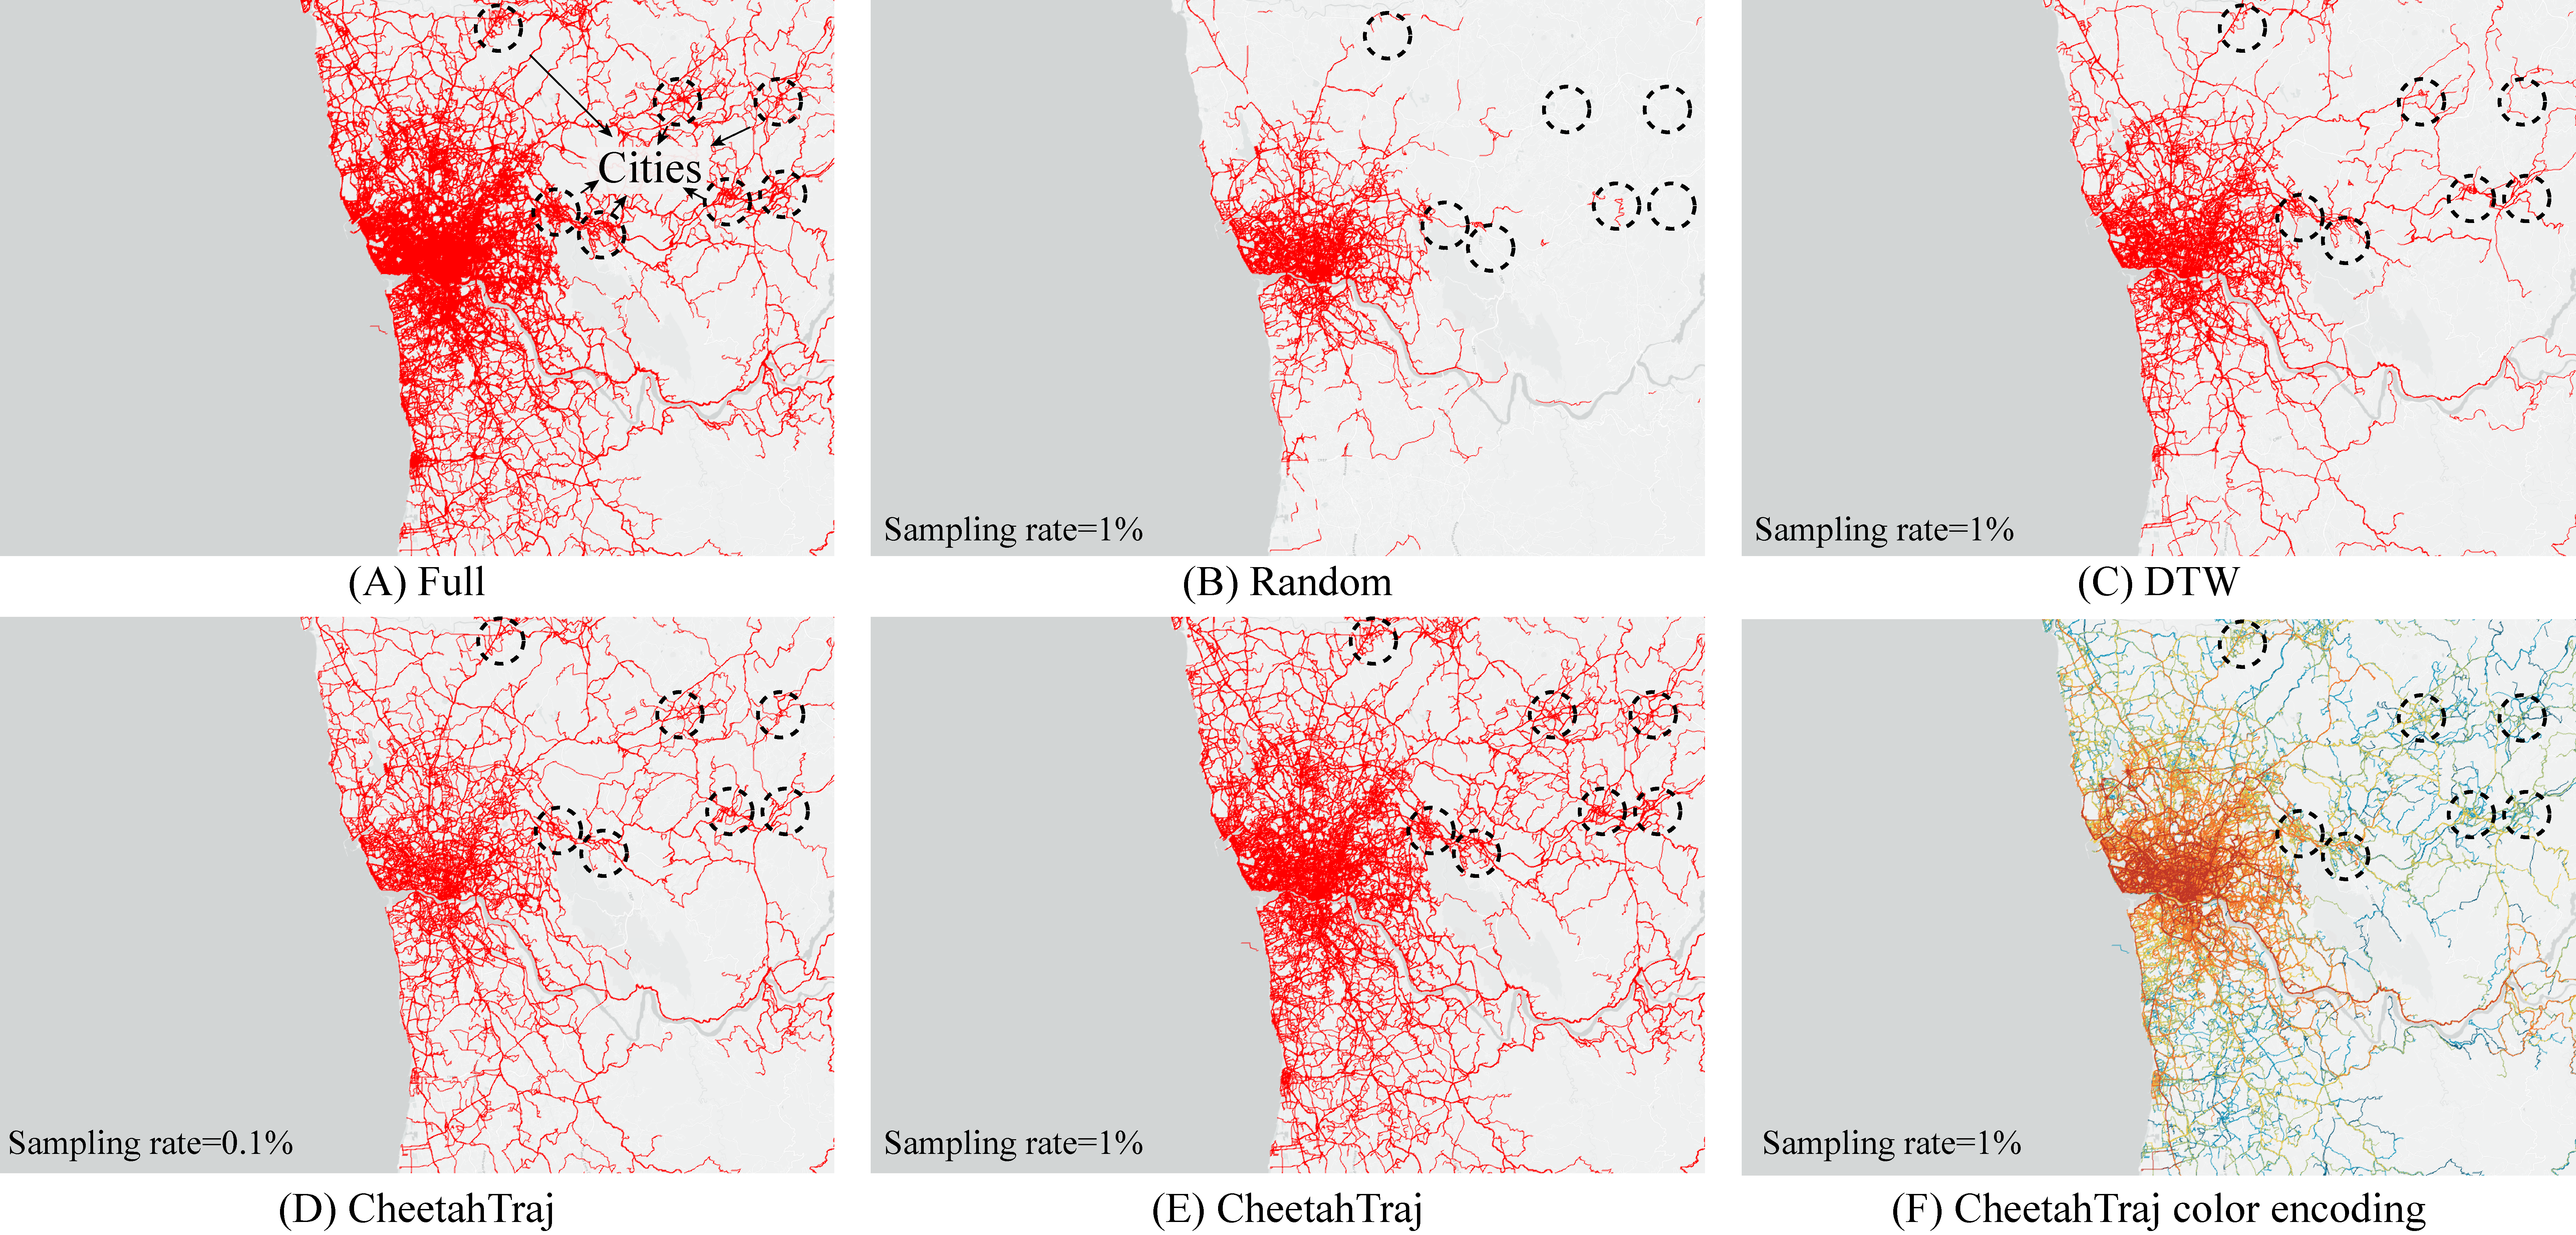
\includegraphics[width=0.98\textwidth]{pictures/case_study_icde/case_study_overview.pdf}
	\trim
	\caption{Effectiveness of $\avats$ at overview visualization in \pt{}.}
	\label{fig:overview}
	\trim \trim
\end{figure*}

\stitle{Ad-hoc sampling has poor visual quality} Sampling techniques are widely used to accelerate large-scale data analysis in both database and visualization communities~\cite{qin2020making,DBLP:conf/sigmod/DingHCC016,DBLP:journals/pvldb/KimBPIMR15,park2016visualization}. By selecting a subset of the trajectories in the target region for visualization, sampling can reduce both visualization time and visual clutter. One such example is ScalaR~\cite{battle2013dynamic}, which employs a reduction layer between the visualization layer and the data management layer. The reduction layer samples records \textit{uniformly at random} (denoted as $\rand$) when the query results are too large. However, $\rand$ has poor visual quality as its visualization could be significantly different from the ground-truth. We provide such an example in Figure~\ref{fig:overview}(B), where $\rand$ fails to include trajectories in the sparse areas of Figure~\ref{fig:overview}(A). Another natural idea is to sample trajectories with good diversity and we develop such a baseline using the famous Dynamic Time Warping (DTW) distance between trajectories~\cite{borcan2012improving}. As shown in Figure~\ref{fig:overview}(C), $\mathsf{DTW}$ provides better visualization than $\rand$ but there are still obvious differences between $\mathsf{DTW}$ and the ground-truth in Figure~\ref{fig:overview}(A). Without explicit visual quality guarantee, sampling trajectories in ad-hoc ways may produce visualizations with poor quality and mislead visual exploration.

% for trajectory
%
% basic idea
%
%for large-scale trajectory data visualization, generating visualizations that is significantly from the ground-truth. Take Figure~\ref{fig:overview}(B) for example, they are the visualization results generated by $\rand$ on the \pt{} taxi trajectory dataset with sampling rate  $1\%$. Obviously, it is very different from the visualization of the full \pt{} dataset in Figure~\ref{fig:overview}(A), since the random sampling method is easily ignore the data patterns in the spare areas.  Another basic idea of the data reduction is to iteratively remove the trajectories \QM{which have the least impact of the whole visualization}~\cite{borcan2012improving}. Thus impact of a trajectory can be evaluated by sum of the distance(DTW or Fréchet distance) to all other trajectories. As shown by Figure.~\ref{fig:overview}, the visualization generated $\baseline$ is much better than $Rand$ by preserve more trajectories in the sparse region, but the general structure is still missing because it cannot theoretically guarantee the visual quality. Moreover the pairwise distance calculation for large trajectory dataset is very time consuming, which always needs days of preprocessing for millions of trajectories.

%VLDB
%Sampling techniques are widely used for large-scale data analysis in both database and visualization communities~\cite{qin2020making,DBLP:conf/sigmod/DingHCC016,DBLP:journals/pvldb/KimBPIMR15,park2016visualization}. By sampling a subset of records from the raw large-scale dataset, it helps to reduce the rendering latency on graphics devices for visualization. One such example is ScalaR~\cite{battle2013dynamic}, which employs a reduction layer between the visualization layer and the data management layer. The reduction layer samples records \textit{uniformly at random} (denoted as $\rand$) when the query results are too large. However, $\rand$ does not work well for large-scale trajectory data visualization as it cannot provide fidelity guarantee. Take Figure~\ref{fig:teaser}(B) and (C) for example, they are the visualization results generated by $\rand$ on the \pt{} taxi trajectory dataset with sampling rate $0.1\%$ and $1\%$, respectively. Obviously, both of them are very different from the visualization of the full \pt{} dataset in Figure~\ref{fig:teaser}(A).


\stitle{The $\avats$ framework} We explore novel algorithm and efficient index jointly in the $\avats$ framework to provide visualizations with high quality and low latency. To conduct quality guaranteed sampling, we first propose a novel pixel-based \textit{visual quality function} to measure how similar an approximate visualization is to the ground-truth. We also show that it is NP-hard to select an optimal set of trajectories that maximize the visual quality function. Next, we devise a \textit{visual quality guaranteed sampling algorithm} named $\vats$, which provides theoretical visual quality guarantee for the sampled trajectories. Then, we \textit{tackle the visual clutter problem} by taking data distribution and human perception into consideration in an advance algorithm named $\vatss$. To avoid running the somehow complex $\vatss$ algorithm on-line for interactive visual exploration, we design an $\invQ$-tree index based on quad-tree. $\invQ$-tree allows to directly use the sampling results computed in an offline index building phase and provides quality guaranteed trajectory samples for an arbitrary target region.




%VLDB
%In this work, we set out to design efficient sampling algorithms that provides visual fidelity guarantee for line-based large-scale trajectory visualization. This goal leads to three research problems: (i) \emph{how to measure the visual fidelity of one visualization result?} (ii) \emph{how to devise an efficient sampling algorithm that provides  guaranteed visual fidelity?} (iii) \emph{how to tackle the visual clutter problem in large trajectory visualization?} To address these problems, we first propose a novel pixel-based \textit{visual fidelity loss function} to formally measure the difference between two visualizations. We then show that it is NP-hard to select a sized-$k$ sample of the trajectories to minimize the visual fidelity loss function. Next, we devise an \textit{efficient approximate algorithm }named $\vats$, which provides theoretical visual fidelity guarantee for the sampled results. Last, we \textit{explicitly tackle the visual clutter problem} by taking data distribution and human perception characteristics into consideration in an advance algorithm named $\avats$.

%In this work, we propose visual fidelity-guaranteed sampling approaches for the line-based trajectory visualization problem.
%The technical challenges of our proposal are
%(i) \emph{how to define visual fidelity of visualization result theoretically?}
%(ii) \emph{how to devise an efficient sampling algorithm which offers visual fidelity guarantee on the visualization result?}
%and (iii) \emph{how to overcome the visual clutter in large trajectory visualization?}
%Specifically, we first propose a novel pixel-based visual fidelity loss function between two visualization results formally.
%With the visual fidelity loss function, we then prove it is NP-hardness to select a sized-$k$ subset of trajectories which has the minimal visual fidelity loss.
%Next, we devise an approximate algorithm $\vats$ which returns a sized-$k$ subset of trajectories and offers theoretical visual fidelity guarantee on the returning result.
%Last, we address the visual clutter issue explicitly by taking data distribution and human perception capability into consideration in the advance approach $\avats$.



We conduct extensive case study, user study and quantitative performance evaluation to validate the visualization quality and efficiency of the $\avats$ framework. The case study shows that $\avats$ consistently provides high quality visualizations for both large target regions and small target regions. The user study with 35 participants confirms that $\avats$ effectively reduces visual clutter and produces visualizations that are plausible to human inspectors. The quantitative performance evaluation shows that $\avats$ provides good visual quality by sampling only a small number of trajectories. In addition,  $\avats$ produces high quality visualizations for arbitrary target regions in less than 1 second for all 3 experiment datasets and the visualation delay is below 0.1 second in most cases.


We illustrates the merits of our $\avats$ framework in Figure~\ref{fig:overview}. Figure~\ref{fig:overview}(D) and (E) are the visualizations produced by $\avats{}$ on the \pt{} dataset with sampling rate $0.1\%$ and $1\%$, respectively. Compared with uniform random sampling (i.e., $\rand$) and diversity based sampling (i.e., $\mathsf{DTW}$) in Figure~\ref{fig:overview}(B) and (C), Figure~\ref{fig:overview}(D) and (E) are obviously more similar to the full dataset visualization in Figure~\ref{fig:overview}(A).
Figure~\ref{fig:overview}(F) is produced by $\avats{}$ using the same parameters as Figure~\ref{fig:overview}(E) but the trajectories are colored according to their algorithm-generated representativeness (warmer color means more representative). Compared with Figure~\ref{fig:overview}(A), the main routes in the dense region can be identified much more easily, which shows that $\avats{}$ effectively reduces visual clutter. Last but not least, it takes $\avats{}$ only 0.116 seconds and 0.339 seconds to generate Figure~\ref{fig:overview}(D) and (E), respectively, while the full visualization in Figure~\ref{fig:overview}(A) takes 16.154 seconds.


% The advantage of our proposals over $\rand$ is also consistent across different zoom levels, e.g., Figure~\ref{fig:overview}(E) vs. Figure~\ref{fig:overview}(C) at level 11, and Figure~\ref{fig:overview}(I) vs. Figure~\ref{fig:overview}(H) at level 15. Figure~\ref{fig:overview}(F) is produced by our $\avats{}$ algorithm using the same parameters as Figure~\ref{fig:overview}(E) but the trajectories are colored according to their algorithm-generated representativeness (warmer color means more representative). Observe that the visual clutter problem in Figures~\ref{fig:overview}(A) and (E) are significantly alleviated in Figure~\ref{fig:overview}(F) with color encoding. This advantage is even more prominent when comparing Figure (I) with Figure (G) and (H).




%Figures~\ref{fig:teaser}(D) and (E) show the visualization results of our proposal $\avats{}$ on \pt{} taxi trajectory dataset with {the} sampling rate $0.1\%$ and $1\%$, respectively.
%Comparing with the corresponding visualization results of uniform random sampling method $\rand$ in Figure~\ref{fig:teaser}(B) and (C),
%the superiority of $\avats$ is obvious.
%% Obviously, the visualization fidelity of them are much better than the uniform random sampling visualization results with the same sampling rates, see Figure~\ref{fig:teaser}(B) and (C).
%Figures~\ref{fig:teaser}(F) is the returning result of our proposal, which colors the trajectories {according to the trajectory representativeness}.
%It has the same parameters of Figure~\ref{fig:teaser}(E).
%Visually, the visual clutter issue in Figures~\ref{fig:teaser}(A) and (E) are alleviated in Figure~\ref{fig:teaser}(F).
%In addition, our proposals are robustness with different zoom levels.
%%Figure~\ref{fig:teaser}(G), (H), and (I) depict the visualization results of the \pt{} dataset, the returning result of uniform random sampling $\rand$ and the returning result of $\avats$ with color encoding at zoom-level 15, for example, we can obtain them by zooming in the visualization result in Figure~\ref{fig:teaser}(A), (C), and (F), respectively.
%Consider the visualization results in Figures~\ref{fig:teaser}(G), (H), and (I) with zoom level 15.
%Intuitively, the visualization result of our proposal $\avats$ in Figure~\ref{fig:teaser}(F) outperforms the uniform random sampling $\rand$ in Figure~\ref{fig:teaser}(H) significantly.
%It even performs better than Figure~\ref{fig:teaser}(G), the visualized result of the \pt{} dataset, as it reduces visual clutter in Figure~\ref{fig:teaser}(G) by using color encoding scheme to capture the representativeness of different trajectories.

To sum up, our technical contributions in this paper include:
%\setlist{nolistsep}
%\begin{itemize}[noitemsep]
\squishlist
  \item We formulate the visual quality optimal trajectory sampling problem for large-scale trajectory data visualization, and prove that it is {NP-hard} (Section~\ref{sec:pro}).
  \item We devise an approximate algorithm $\vats$ for the visual quality guaranteed sampling problem. $\vats$ is further improved with $\vatss$ by considering data distribution and human perception (Section~\ref{sec:sol}).
  \item We propose the $\avats$ framework, which jointly uses the aforementioned algorithms and tailored index to achieve both quality and efficiency in large-scale trajectory data visualization (Section~\ref{sec:cheetahtraj}).

   %We conduct extensive experiments on real-world trajectory datasets to demonstrate the superiority of our proposals in Section~\ref{sec:exp}. In particular, nearly 200 real users are recruited to test the effectiveness of our methods on three practical applications.
\squishend
%\end{itemize}


This rest of the paper is organized as follows. Section~\ref{sec:rel} introduces related works on trajectory visualization and interactive visualization. The quality optimal trajectory sampling problem is formulated and analyzed in Section~\ref{sec:pro}. Section~\ref{sec:sol} presents our $\vats$ and $\vatss$ algorithm for quality guaranteed trajectory sampling. Section~\ref{sec:cheetahtraj} elaborates the $\avats$ framework. The experiment results are presented in Section~\ref{sec:exp}. Section~\ref{sec:con} draws the concluding remarks.


% in Section~\ref{sec:pro}

%Our proposal demonstrates their superiority over existing methods
%With the same sampling set size($1\%$), the proposed method generates a higher-fidelity visualization and .

%With the loss function, we analyze the hardness of the problem, and devise a visual quality guaranteed sampling algorithm for it.
%Figure~\ref{fig:compare} depicts an comparison among the ground truth,  uniform random sampling and our proposed method.
%With the same sampling set size($1\%$), the proposed method generates a higher-fidelity visualization and support the multi-resolution very well.
%At last, color encoding are applied to enhance the distribution of trajectories.

%


%\TB{Visualizing a large collection of trajectories are used frequently in map service or smart city applications.}
%The most popular and conventional method is the line-based visualization~\cite{chen2015survey}: connecting the passing points of movement objects by polylines.
%To handle the big dataset, many visualization products such as Spotfire~\footnote{\url{https://www.tibco.com/products/tibco-spotfire}}
%and Tableau~\footnote{\url{https://www.tableau.com/}} support advanced database management systems as a ``backend'' for the efficient data processing the query.
%The current visualization tools always don't scale well for the presentation of very large trajectory dataset due to the two challenges,
%visual clutter and limited rendering speed, which hinders the abilities of human-users for interactively exploring the dataset and identifying the movement patterns.
%In recent years, most of the visualization research works mainly try to address the visual clutter issue by proposing new techniques such as the
%spatial aggregation~\cite{zeng2013visualizing, von2015mobilitygraphs}, edge bundling~\cite{zeng2019route, thony2015vector} and density map~\cite{lampe2011interactive, scheepens2011interactive}.
%Instead, in this paper, we focus on the challenge of inefficient rendering in the large trajectory dataset by involving data sampling techniques.

%It is time consuming to generate very simple visualization when the data size become very large. Using Porto taxi data ~\footnote{\url{http://www.geolink.pt/ecmlpkdd2015-challenge/dataset.html}} as an example, Table~\ref{table:rendering_time} demonstrates the rendering time at each dataset size. \ZW{shall also mention which rendering toolkit is used here.} It shows that normal method takes more than 14 minutes (\ZW{seconds?}) to generate the graphics for 1 million trajectories, which is far beyond the human-acceptable response time for the interactive exploration~\cite{shneiderman1984response}.
%One work closely related to ours is ScalaR~\cite{battle2013dynamic}, which adds a reduction layer between visualization layer and data management layer. The reduction layer uses an uniform random sampling method to sample data once the query results are large enough, thus to reduce the amount of data to be visualized.
%Further more, Park et al. propose VAS~\cite{park2016visualization} which implements new sampling techniques to guarantee the visual quality.
%However, these sampling techniques are designed for the simple dataset, and have been approved effective in scatter plot or map plot.
%However, the trajectory sampling is more challenge due to the complexity of data form(e.g. varying lengths, lack of compact representation, difficulty in measuring the similarity) that makes traditional density-biased sampling techniques inappropriate.
%A naive solution to employ sampling idea for large-scale trajectory visualization problem is randomly selecting several trajectories from the data set then visualize it by graphics device.
%However, the visualization result may be not acceptable by the user because of the visual information loss in the sparse distributed regions.





%
%\begin{figure}[t]
%	\centering
%	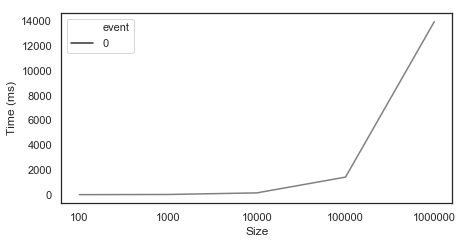
\includegraphics[width=0.4\textwidth]{pictures/introduction/timesize.png}
%	\vspace{-5mm}
%	\caption{The latency time for generating line-based visualization at each datasize.}
%	\vspace{-5mm}
%	\label{fig:rendering_time}
%\end{figure}




%The major challenges to design visual quality guaranteed sampling method are:
%(I) how to define visual quality theoretically? (II) how to guarantee the quality of the sampling-based visualization result?
%\TB{In this work, we study how to reduce the rendering time and preserve the visual quality for the large-scale trajectory visualization.}
%We extend the motivation of visualization-aware sampling to trajectory dataset and propose a novel sampling strategy, \textbf{v}isualization \textbf{a}ware \textbf{t}rajectory \textbf{s}ampling(VATS), that produces high-visual-quality line-based trajectory visualization at different zooming resolutions.
%%\QM{In this paper, we first proposed the visual fidelity loss function which effectively evaluates the visual loss of the sampling method. Then we minimize the loss function by transforming this problem to an optimization problem. Several solutions for efficiently solving the optimization problem are discussed.}
%We first format visual quality by defining the loss function between the visualization results of the whole dataset and sampled dataset.
%With the loss function, we analyze the hardness of the problem, and devise a visual quality guaranteed sampling algorithm for it.
%Figure~\ref{fig:compare} depicts an comparison among the ground truth,  uniform random sampling and our proposed method.
%With the same sampling set size($1\%$), the proposed method generates a higher-fidelity visualization and support the multi-resolution very well.
%At last, color encoding are applied to enhance the distribution of trajectories.
%
%\begin{figure}[t]
%	\centering
%	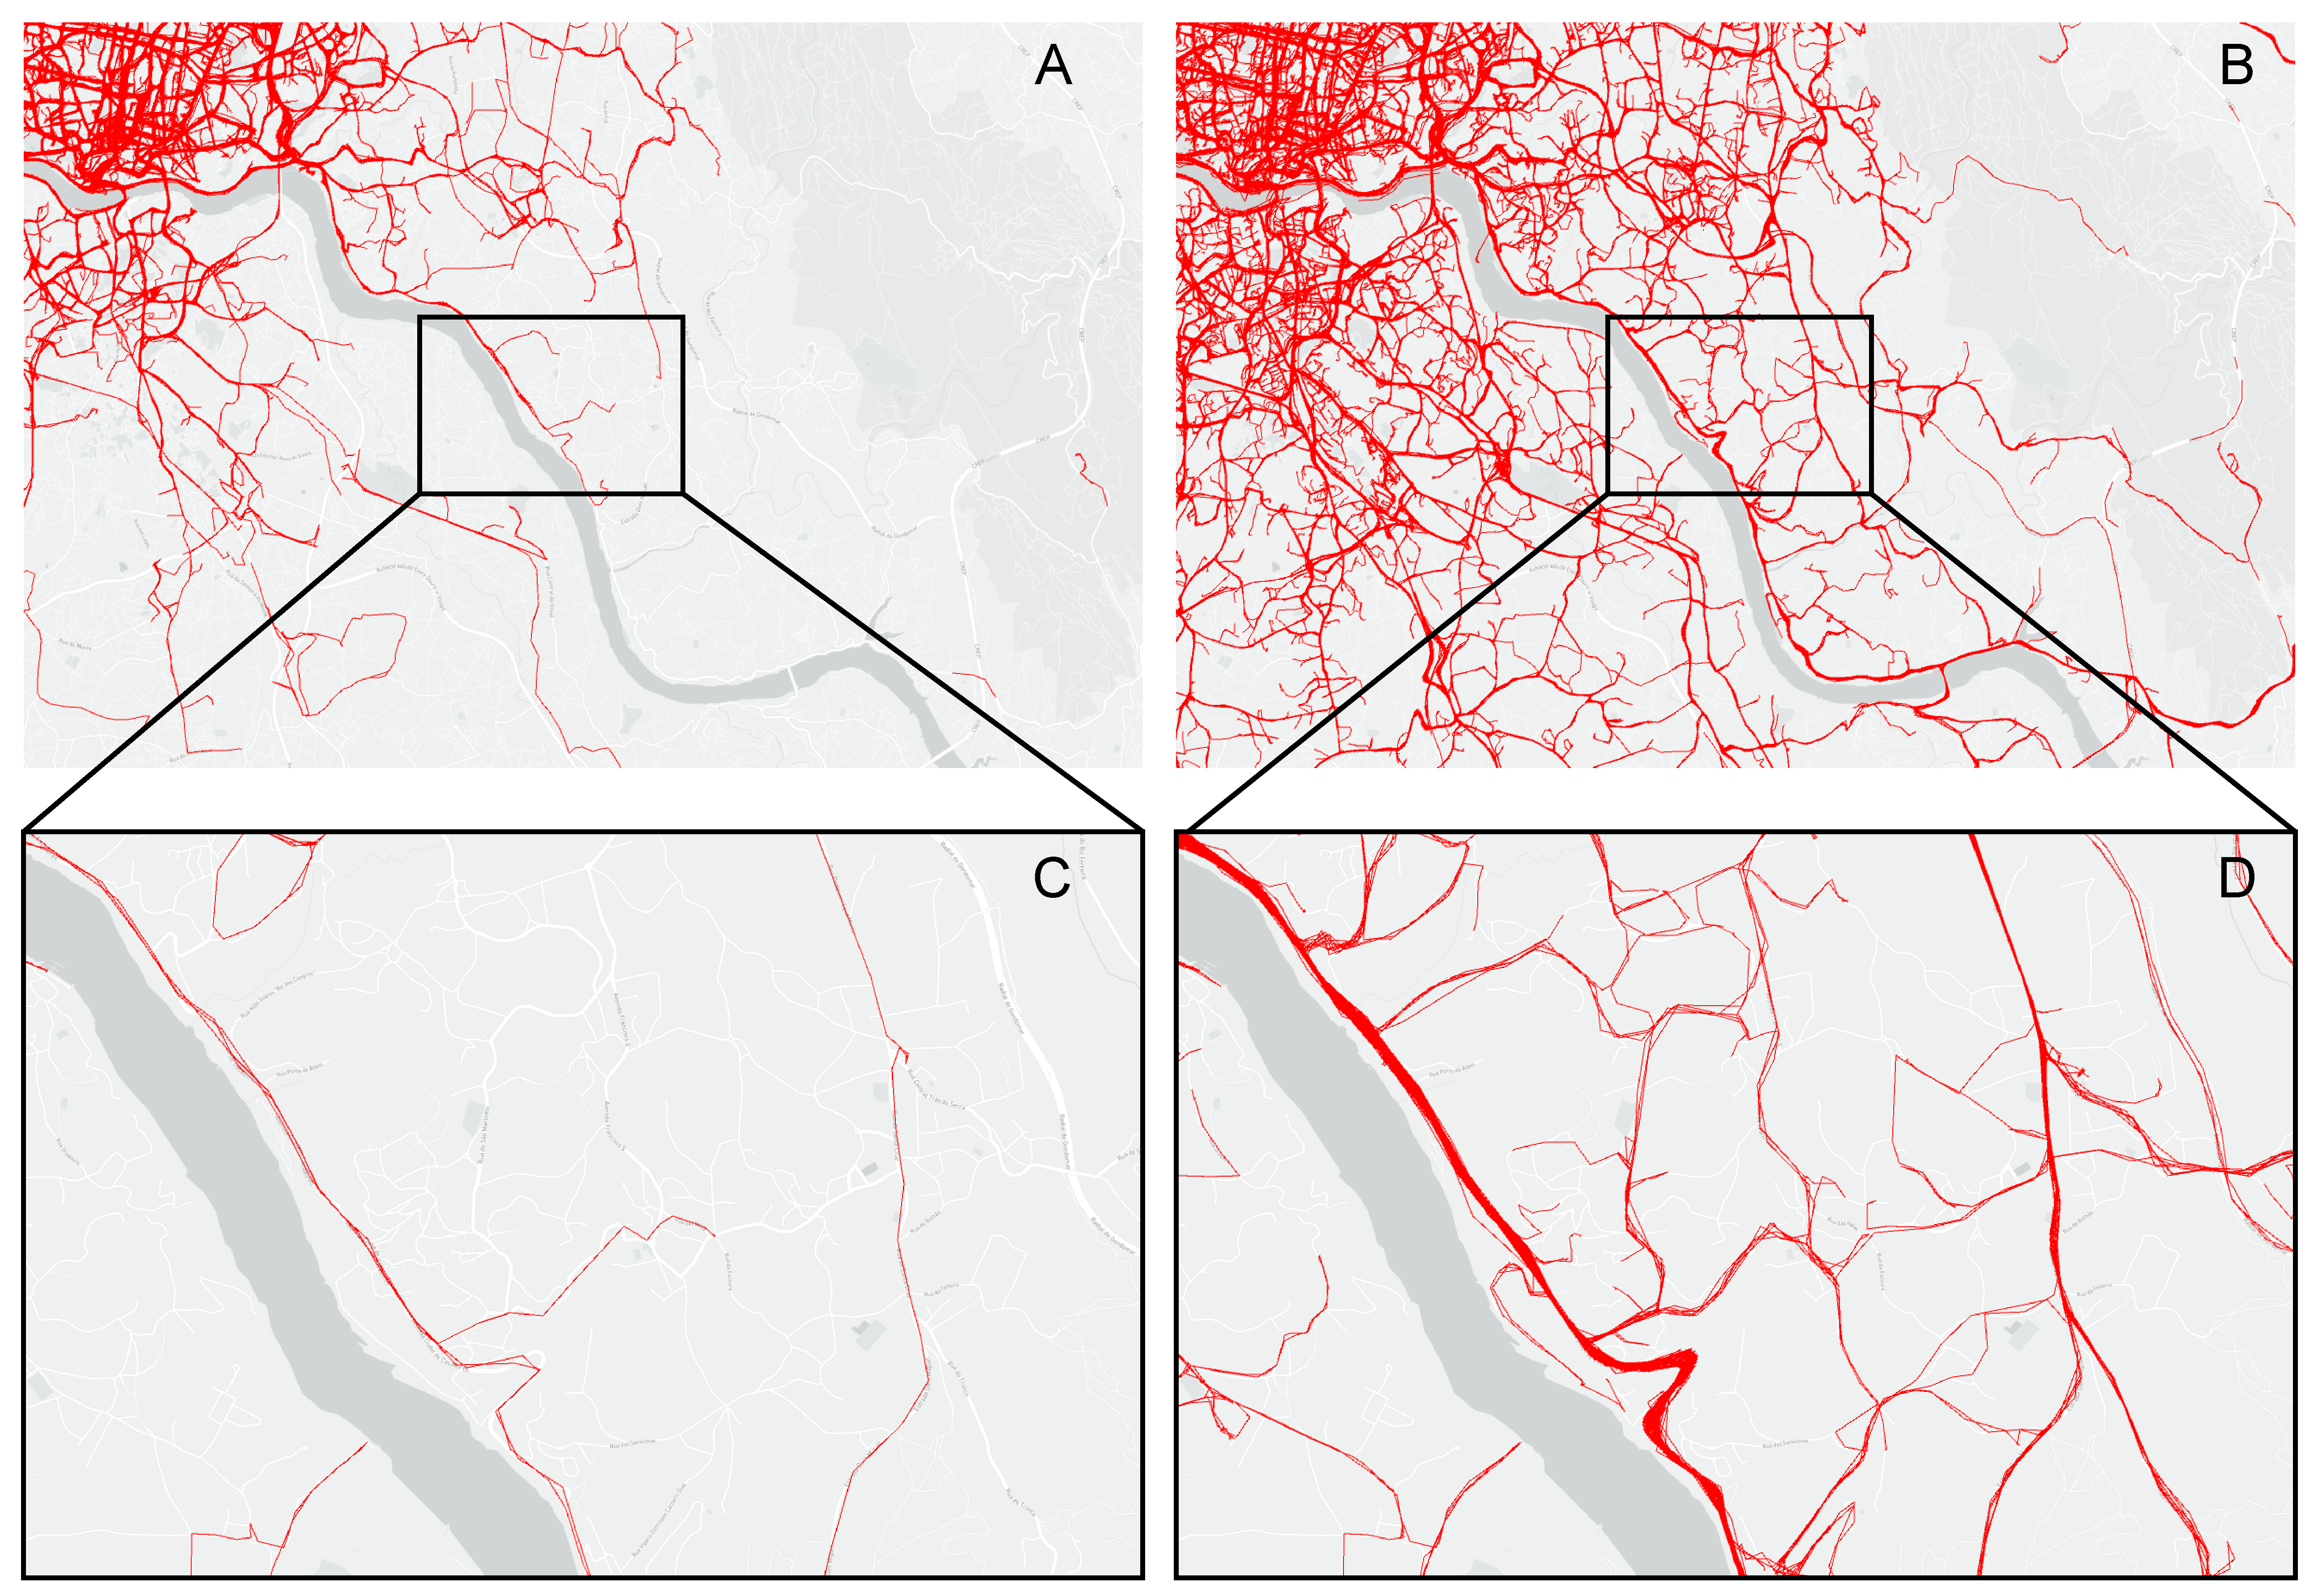
\includegraphics[width=0.44\textwidth]{pictures/introduction/effectiveness.pdf}
%	\vspace{-3mm}
%	\caption{Trajectory sampling generated by uniform random sampling(A,C) and VQGTS(B,D) at same sampling rate. In both high-level(A,B) and low level(C,D) view, our approach preserved more detail information about the trajectories especially for the sparse regions.}
%	\vspace{-5mm}
%	\label{fig:compare}
%\end{figure}
%

%
% \Bo{we can keep it at technical report.}
%The remainder of this paper is organized as follows. Section~\ref{sec:rel} discusses the related work, and Section~\ref{sec:pro} formally formulates our problem and analyze its hardness. Section~\ref{sec:sol} presents our approximate solution for the problem along with the optimization techniques. The advanced solution for visual clutter is introduced in Section~\ref{sec:aa}. Section~\ref{sec:exp} elaborates the extensive experimental studies. Section~\ref{sec:con} concludes this paper and highlights possible future directions.


%Section~\ref{sec:pro} formulates our problem and analyze its hardness.
%Section~\ref{sec:sol} provides an approximate solution for it, together with a suite of optimization techniques.
%Section~\ref{sec:aa} proposes an advanced solution for our problem.
%Section~\ref{sec:exp} elaborates our extensive experimental studies and our findings in detail.
%Section~\ref{sec:con} concludes this work and highlights the promising future directions.



\section{Background and Related work}\label{sec:rel}
%In this section, we survey previous work and focus on the most relevant pieces.
%Section~\ref{sec:trajvisana} and ~\ref{sec:interactive} summarize the related works in trajectory visual analysis and interactive data visualization for large dataset, respectively.

In this part, we survey related works on \textit{trajectory visualization methods} in Section~\ref{sec:trajvisana} and \textit{interactive data visualization for large datasets} in Section~\ref{sec:interactive}, respectively.

\subsection{Trajectory Visualization Methods}\label{sec:trajvisana}
A trajectory is a sequence of spatial locations (e.g., GPS positioning results) and trajectories are the most common representations of object movements. Existing trajectory visualization methods can be classified into three categories according to the form of visualization~\cite{chen2015survey}, i.e., \textit{point-based}, \textit{region-based}, and \textit{line-based}. We give a brief introduction to these methods and refer the interested readers to~\cite{chen2015survey} for more detailed discussions.


Point-based visualization plots the locations in the trajectories independently and captures the overall spatial distribution of the moving objects. Many density-based methods~\cite{liu2013vait,yang2016exploring,chae2014public,borruso2008network}, 
%~\cite{liu2013vait,yang2016exploring,chae2014public,xie2008kernel, borruso2008network}
e.g., kernel density estimation, are applied in point-based visualization to preserve the spatial distribution. Region-based visualization slices the entire region into sub-regions and visualizes the aggregated information in each sub-region~\cite{guo2009flow,von2015mobilitygraphs}.
%~\cite{guo2009flow,wood2010visualisation,von2015mobilitygraphs}
As region-based visualization focuses on aggregated statistics, it is most effective in capturing macro-patterns. In this work, we focus on line-based visualization, which uses polylines to connect the locations in each trajectory and shows the trace of object movements (see an example in Figure~\ref{fig:line}). As line-based visualization preserves the continuous movement information of objects~\cite{guo2011tripvista,hurter2009fromdady}, it is widely used in many visual analysis applications such as traffic management, urban planning, and route recommendation. However, line-based visualization is known to suffer from severe visual clutter, especially when the dataset is large. Several techniques have been proposed to alleviate visual clutter, such as clustering-based techniques~\cite{von2015mobilitygraphs}
%~\cite{ferreira2013vector, rinzivillo2008visually, von2015mobilitygraphs}
and advanced interaction techniques~\cite{ferreira2013visual}.
%~\cite{kruger2013trajectorylenses, ferreira2013visual}



\subsection{Interactive Visualization for Large Datasets}\label{sec:interactive}
%With the recent advancement of location-acquisition technology, the size of available trajectory dataset becomes extremely huge.
%For example, the operating taxis in Shenzhen generate {$\sim$}9.3GB trajectory data per day.
%Figure~\ref{fig:framework} illustrates the architecture of interactive visualization systems for large datasets,
%e.g., Spotfire~\cite{Spotfire}, Tableau~\cite{Tableau}, ATLAS~\cite{chan2008maintaining}, and Viate~\cite{yang2019vaite}.
%{It} consists of three layers: the user interface in front-end, the optimization techniques in middle-layer, and the (cloud-based) database management system in the back-end.
%{Typically, the researchers in visualization community focus on improving the effectiveness of data visualization at the front-end,
%e.g., designing novel visualization method D3~\cite{d3} to assist data analysts to obtain data insights effectively.}
%For the researchers in database community, they are working on the efficiency aspect for large data processing,
%e.g., devising big data processing system Spark~\cite{spark} for efficient query processing at back-end.
%In recent years, both visualization and database communities are dedicating to advance the techniques in interactive visual analysis for large-scale dataset,
%e.g., the optimizations in the middle-layer (see Figure~\ref{fig:framework}).
%We briefly elaborate these optimization techniques {in this section}.






Figure~\ref{fig:sys_framework} illustrates a general architecture of interactive visualization systems,
e.g., Spotfire\footnote{\url{https://www.tibco.com/products/tibco-spotfire}}, Tableau\footnote{\url{https://www.tableau.com/}}, ATLAS~\cite{chan2008maintaining}, Viate~\cite{yang2019vaite} and Marviq~\cite{dong2020marviq}.
There are typically three layers: user interface in the front-end layer, optimization techniques in the middle-layer, and database management system (usually cloud-based) in the back-end layer. The visualization community usually focuses on improving the effectiveness of data visualization at the front-end, e.g., designing novel visualization methods/toolkits such as D3\footnote{\url{https://d3js.org/}} to enable data analysts to effectively gain insights from data. 
The database community usually aims to improve query efficiency, e.g., devising big data systems such as Spark\footnote{\url{https://spark.apache.org/}} for efficient data processing at the back-end. 
With the popularization of location-acquisition devices, the scale of trajectory datasets can be extremely large. For example, the taxis in Shenzhen generate {$\sim$}9.3GB trajectory data per day. However, visualization generation has a long latency for large datasets due to heavy data processing/graphic rendering, which harms the responsiveness of interactive visualization. Therefore, both the visualization and database communities began to advance techniques in the middle-layer to reduce visualization latency for large datasets. We briefly elaborate these techniques as follows.


\begin{figure}
	\centering
	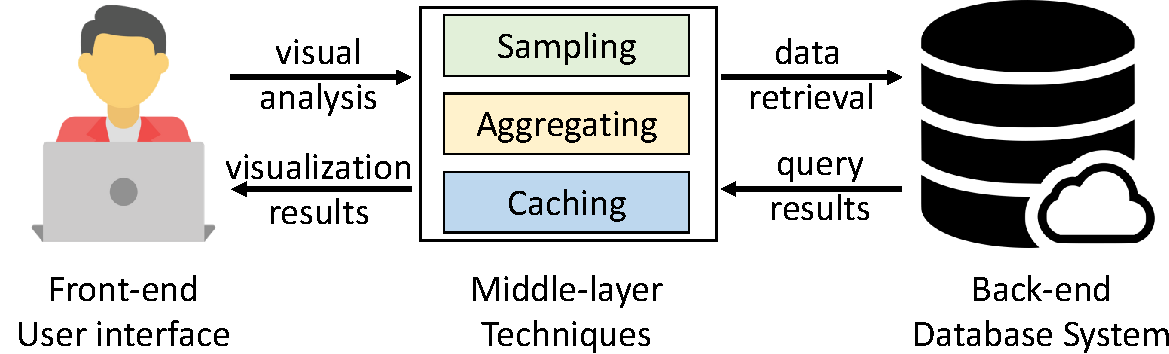
\includegraphics[width=0.45\textwidth]{pictures/framework/framework.pdf}
	\trim
	\caption{System architecture for interactive visualization.} \label{fig:sys_framework}
    \trim \trim
\end{figure}


\stitle{Aggregation-based techniques}
%{Aggregating-based techniques pre-process raw data with aggregation techniques (e.g., clustering) in the middle-layer, and yield fewer rendering objects for interactive visual analysis.}
%Returning to the trajectory visual analysis,
These works divide the {entire area} into basic units and visualize the aggregated information of the trajectories for each unit~\cite{wood2010visualisation,guo2009flow,von2015mobilitygraphs}. For more details on aggregation-based techniques, we refer the reader to~\cite{andrienko2008spatio,adrienko2010spatial}. Our problem and solutions are different from these works as we focus on visualizing the raw trajectories, instead of aggregated statistics.
%However, aggregating-based methods will cause information loss definitely.
%For instance, the continuous spatial traces of the moving objects are always missing and the rarely appeared trajectories are easily to be ignored.






\stitle{Sampling-based techniques} Sampling is widely used in both visualization and database communities ~\cite{battle2013dynamic,rapp2019void,chen2014visual,yu2020turbocharging,park2016visualization,qin2020making,DBLP:conf/sigmod/DingHCC016,DBLP:journals/pvldb/KimBPIMR15}. These works try to reduce the dataset to a subset with some special characteristics: such as blue noise property~\cite{rapp2019void}, multi-class property~\cite{chen2014visual} or maximize some user-defined quality~\cite{yu2020turbocharging}. The work most relevant to ours is~\cite{park2016visualization}, which is designed for scatter plots (a form of point-based visualization). It reduces the number of points in a plot while preserving the spatial distribution of the points in the original dataset. The techniques in~\cite{park2016visualization} cannot be applied to our trajectory visualization problem
as trajectory is more complex than individual scatter points (e.g., the order of GPS points is essential and the trajectories could have a large variance in length). Some works simplify a trajectory by sampling important points to reduce data size~\cite{zhang2018trajectory,2018arXiv180303550V} or alleviate visual clutter~\cite{borcan2012improving, 6851202}. These works are orthogonal to ours as we are sampling complete trajectories instead of points in a trajectory.



%It's worth to mention the area of trajectory simplification~\cite{zhang2018trajectory, 2018arXiv180303550V} which is orthogonal to our proposals. Trajectory simplification tries to simplify a single trajectory by preserving the important points in a trajectory, which can be used to reduce the data size~\cite{zhang2018trajectory} or alleviate  the visual clutter~\cite{borcan2012improving, 6851202}. We refer the audience to~\cite{zhang2018trajectory} for more details.

%are well-studied in the interactive visualization problems with large-scale input data.
%It is
%In particular, ~\cite{chen2014visual} devised a sampling algorithm to preserve the meaningful data items.
% according to the analyzing requirement such as the multi-class data analysis and hierarchical exploration.

%(i) the complexity of the trajectories~\cite{pelekis2010unsupervised}, and (ii) the loss function and its corresponding solutions are specified for scatter plot, not applicable for line-based trajectory visualization.
%For trajectory visual analysis,  most of the existing trajectory sampling techniques (if not all) cluster the trajectories at first,
%then select the most representative trajectories from each cluster and visualize them.
%It is impractical to provide interactive visualizations for real-world applications as
%trajectory clustering is still an open problem in both database and visualization communities~\cite{panagiotakis2011segmentation,agarwal2018subtrajectory}.

%as
%(i) the trajectory similarity computation and clustering algorithms are very expensive~\cite{pelekis2007similarity},
%and (ii) the



\stitle{Caching-based and other techniques}
%Caching is commonly used to improve the performance of large data processing system, e.g., search engine~\cite{xu2015diversified}.
Chan et al. propose ATLAS~\cite{chan2008maintaining}, which utilizes caching for efficient data communication between server and client.
ATLAS also exploits a powerful multi-core server to accelerate visual analysis tasks in both the middle-layer and back-end.
Piringer et al.~\cite{piringer2009multi} propose an architecture for interactive visual exploration,
which utilizes multi-core devices and avoids the common pitfalls of multi-threading to provide quick visual feedback.
Our work is orthogonal to these execution optimizations as we mainly focus on the algorithm perspective.

%Current advancing sampling techniques in the visualization domain are mostly
%Some works design advanced sampling algorithms to preserve the meaningful data items according to the analyzing requirement such as the multi-class data analysis and hierarchical exploration~\cite{chen2014visual}. Furthermore, to the usage of more visual channels of the points other than location such as color~\cite{chen2014visual}, size~\cite{woodruff1998constant} and opacity are discussed.
%Closely related to our work, Park et al.~\cite{park2016visualization} proposed the visualization-aware techniques for the scatter plot.
%
%In comparison with the sampling techniques for scatter plot, the trajectory sampling is more challenging because of the complexity of the trajectories~\cite{pelekis2010unsupervised}.
%
%
%Many exiting visual analytics systems leverage powerful database manage system as the backend to facilitate the fast data processing. Based on the solution proposed in ScalaR~\cite{battle2013dynamic}, a common visualization framework involving sampling technique is illustrated as Figure~\ref{fig:framework}, where a sampling layer is set between the backend and frontend. Since the sampling methods are always designed for complicated task, the algorithms may not be efficient enough to support the interactive data exploration. Thus the cache model is always implemented to save the sampling results. In our scenario, the users query large amount of data(e.g. all Shenzhen trajectories in one week) once and then conduct interactive multi-resolution exploration based on the sampled data, thus the method need to guarantee the visual quality well across different resolutions.
%
%Sampling is a delta-facto solution for the problems with big data. Target at the sampling requirement, the naive solutions such as uniform random sampling cannot generate acceptable because the serious visual information loss. In this section, we first define a loss function to evaluate the visual quality between the visualization results between whole dataset and sampled subset. Then we analyze the hardness of the problem and design algorithms for it.
%
%
%\begin{figure}[t]
%	\centering
%	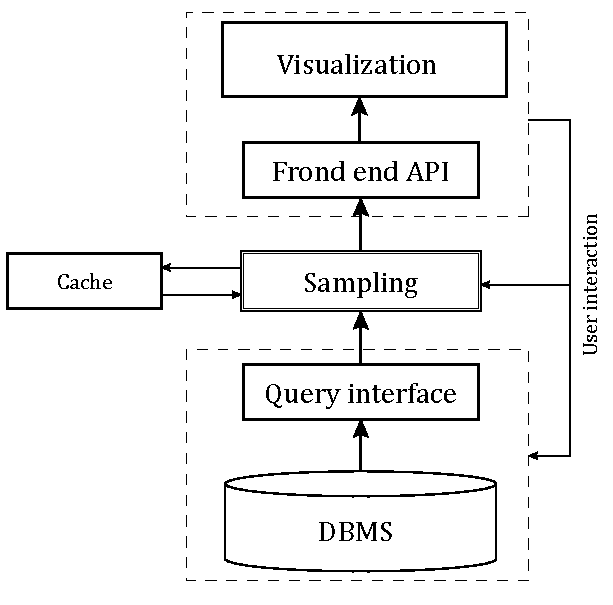
\includegraphics[width=0.3\textwidth]{pictures/framework/DBVAframework.pdf}
%	\vspace{-5mm}
%	\caption{A visualization framework involving sampling layer between the front-end and database management system.}
%	\vspace{-5mm}
%	\label{fig:framework}
%\end{figure}
%

\sstitle{Novelties of our work} To the best of our knowledge, we are the first to formulate the quality optimal trajectory sampling problem to accelerate visualization on large scale datasets. We devise effective algorithms for this problem, which not only provide visual quality guarantee but also reduce the well-know visual clutter in trajectory visualization. Based on these algorithm, we design the $\avats$ framework with a tailored $\invQ$-tree index to produce high quality visualization for arbitrary target region with low latency.


%we are the first to observe that random sampling harms visual quality for large-scale trajectory visualization and formulate the problem of quality-guaranteed sampling. To tackle this problem, we design a complete framework with quality loss function, theoretical quality loss analysis, and algorithm efficiency optimizations. the well-know visual clutter problem of trajectory visualization is also addressed naturally in our sampling framework. Extensive experimental results show that our proposals effectively maintain visual quality and reduces visualization latency at the same time.


%Our work differs from the above researches as we propose visual quality-guaranteed sampling approaches for the large-scale trajectory visualization problem,
%we demonstrate the superiority of our proposals by case-, user- and quantitative- studies in real-world dataset.
%
%Unlike existing line-based visualization techniques, we propose visual quality-guaranteed sampling approaches for line-based trajectory visualization with large-scale input data.
%To the best of our knowledge, it is the first work which offers theoretical visual quality guarantee on the sampling result for large-scale line-based trajectory visualization. 

\section{Problem Formulation}\label{sec:pro}
In this section,
we first formally define the \textit{quality optimal sampling problem} (\prob{}) for large-scale trajectory data visualization in Section~\ref{sec:def},
and then show that it is NP-hard to solve the problem exactly in Section~\ref{sec:hard}.

\begin{figure}
	\centering
	\small
	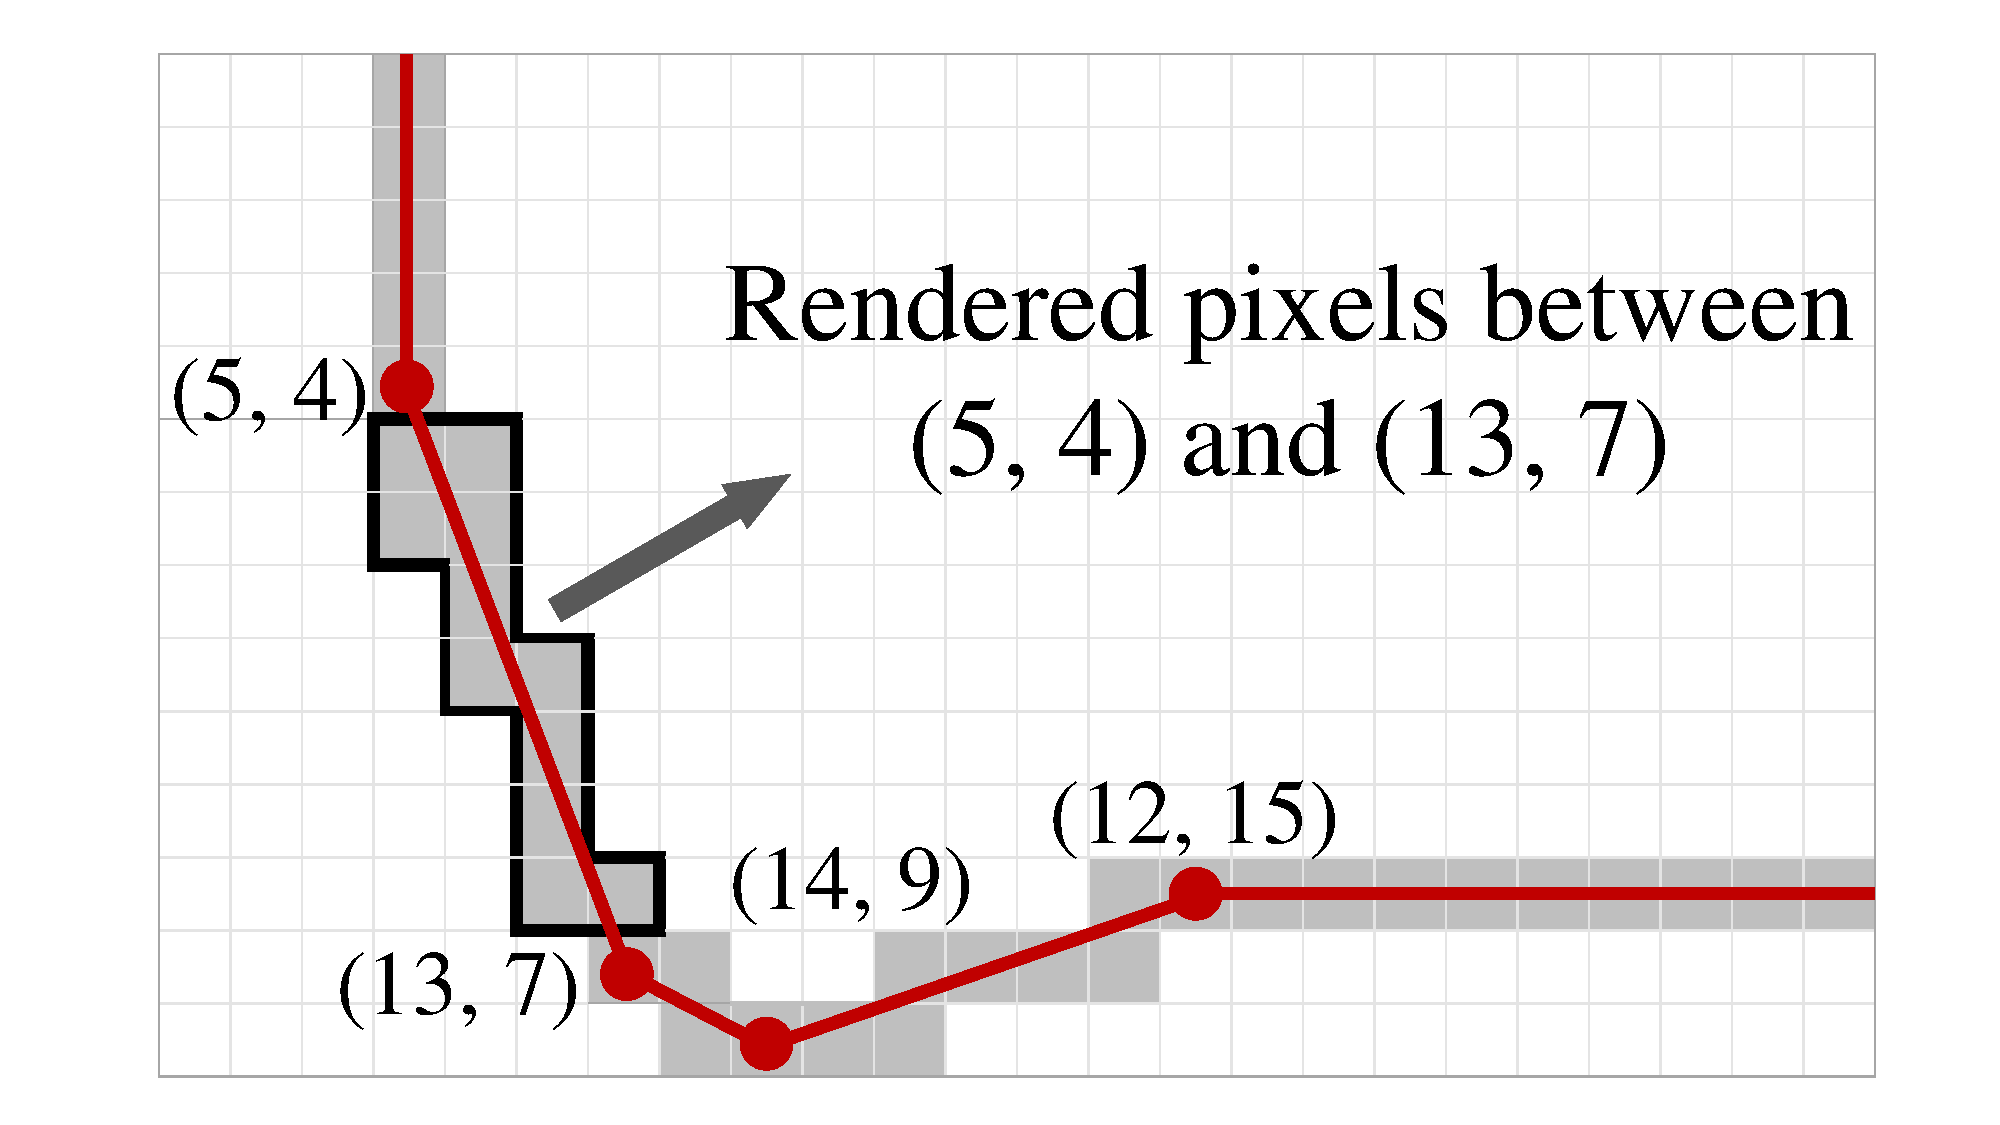
\includegraphics[width=0.5\columnwidth]{pictures/problemsolveing/RenderedPixels}  
    \trim
	\caption{Illustration of line-based trajectory visualization.} \label{fig:line}
    \trim \trim
\end{figure}


\subsection{Problem Definition}\label{sec:def}

We motivate our definition of the \textit{visualization quality function} by introducing how line-based trajectory visualization works.
As elaborated earlier, a trajectory contains a sequence of 2-dimensional locations.
Given an empty canvas (i.e., the screen of a displaying device) with pixels indexed by horizontal and vertical coordinates (i.e., $x$ and $y$), line-based trajectory visualization connects consecutive locations in each trajectory with polylines and marks the pixels passed by these polylines (with a color different from the background).
As shown in Figure~\ref{fig:line}(A), the result of line-based trajectory visualization can be regarded as a 2-dimensional array of boolean variables with 1 indicting that a pixel has been marked.
Alternatively, we can treat a visualization result as a set $\mathcal{S}=\{(x_i, y_i)\}_{i=1}^{n}$ that contains all marked pixels.
This observation leads to the following definition of visualization quality function
\begin{equation}\label{eqref:loss}
\QQ(\mathcal{S}, \mathcal{S}')=\frac{|\mathcal{S} \cap \mathcal{S}'|}{|\mathcal{S}|},
\end{equation}
in which $|.|$ measures the cardinality of a set, $\mathcal{S}$ is the visualization result of the entire trajectory dataset $\mathcal{T}$ while $ \mathcal{S}'$ is the visualization result of some trajectories sampled from $\mathcal{T}$.
As $\mathcal{S}'\subseteq \mathcal{S}$, $\QQ(\mathcal{S}, \mathcal{S}')$ essentially measures the ratio of the pixels in the ground-truth visualization $\mathcal{S}$ that are marked in the approximate visualization $\mathcal{S}'$.
%\footnote{For more general cases with $\mathcal{V}'\not\subset \mathcal{V}$, the quality function can be defined as $\mathsf{q}(\mathcal{V}, \mathcal{V}')\!=\!\frac{|\mathcal{V}-\mathcal{V}'|}{|\mathcal{V}|}$, in which set $\mathcal{V}^\star\!=\!\mathcal{V}-\mathcal{V}'$ contains all distinct elements between $\mathcal{V}$ and $\mathcal{V}'$.}.
This definition matches human visual perception and the approximate visualization $\mathcal{S}'$ will look similar to $\mathcal{S}$ if $\QQ(\mathcal{S}, \mathcal{S}')$ is large.
Sampling reduces the number of trajectories and location points to process, and thus shortens the visualization time.
With the quality function, we define the quality optimal sampling problem as follows.

\begin{problem}[Quality Optimal Sampling Problem, \prob{}]\label{prob:def}
Let the entire trajectory dataset be $\mathcal{T}$ and a sample set that contains some trajectories from $\mathcal{T}$ be $\mathcal{R}$.
Using $\VV(\mathcal{U})$ to denote the visualization result set derived from a trajectory set $\mathcal{U}$, with a sampling rate $\alpha$,
the quality optimal sampling problem finds a set $\mathcal{R}$ that satisfies
	\begin{equation}\label{eq:opp}
	\max_{\mathcal{R} \subseteq \mathcal{T}, |\mathcal{R}| = \lceil \alpha |\mathcal{T}| \rceil} \QQ(\VV(\mathcal{T}), \VV(\mathcal{R}))=\frac{|\VV(\mathcal{T}) \cap \VV(\mathcal{R})|}{|\VV(\mathcal{T})|}.
	\end{equation}
\end{problem}
Note that we are sampling \textit{complete trajectories} instead of \textit{individual locations} in \prob{} such that the lines and orientations in the trajectories are persevered.

Intuitively, given a visualization quality threshold $\tau$, the \prob{} problem can be transformed to find the sampled trajectory set $\mathcal{R}$ with the smallest $\alpha$,
under which provides the quality requirement holds, i.e, $\QQ(\VV(\mathcal{T}), \VV(\mathcal{R})) \!\ge\! \tau$.




\subsection{Hardness Analysis}\label{sec:hard}
We use $t_i\! \in \! \mathcal{T}$ to denote a trajectory in the dataset.
According to the working mechanism of line-based trajectory visualization, $t_i$ corresponds to a set of marked pixels on the canvas in the ground-truth visualization $\VV(\mathcal{T})$ and we also use $t_i$ to denote this set of pixels.
Thus, we have $\VV(\mathcal{T}) = \cup_{t_i \in \mathcal{T}} t_i$ and $\VV(\mathcal{R}) = \cup_{t_i \in \mathcal{R}} t_i$.
We can transform Problem~\ref{prob:def} as follows:

\begin{align}\label{eqn:obj2}
& \max_{\oR \subseteq \D, |\oR| = \lceil \alpha |\mathcal{T}| \rceil}  \frac{|\VV(\mathcal{T}) \cap \VV(\mathcal{R})|}{|\VV(\mathcal{T})|} \\ \nonumber
& \Leftrightarrow \max_{\oR \subseteq \D, |\oR| = \lceil \alpha |\mathcal{T}| \rceil}   |\VV(\oR)|   %\\ \nonumber
 \Leftrightarrow \max_{\oR \subseteq \D, |\oR| = \lceil \alpha |\mathcal{T}| \rceil} | \cup_{t_i \in \oR} t_i |.
\end{align}

%\begin{align}\label{eqn:obj5} \nonumber
%	\min_{\oR \subseteq \D, |\oR| = \alpha |\D|}  \frac{|\V(\D) - \V(\oR)|}{|\V(\D)|}  & \Leftrightarrow \min_{\oR \subseteq \D, |\oR| = \alpha |\D|}   - |\V(\oR)| \\ \nonumber
%	\Leftrightarrow \max_{\oR \subseteq \D, |\oR| = \alpha |\D|}  |\V(\oR)| &  \Leftrightarrow \max_{\oR \subseteq \D, |\oR| = \alpha |\D|} | \cup_{t_i \in \oR} t_i |
%\end{align}

The transformations use the fact that $\VV(\mathcal{R}) \!\subseteq \! \VV(\mathcal{T})$ as $\mathcal{R}\! \subseteq \! \mathcal{T}$, and the ground-truth marked point set $\VV(\mathcal{T})$ has constant cardinality.
The last line shows that \prob{} is equivalent to the famous set cover maximization problem\footnote{\url{https://en.wikipedia.org/wiki/Maximum_coverage_problem}}.
Specifically, given an integer $k$, and a collection of sets $\D = \{t_1, t_2, \cdots, t_n \}$,
set cover maximization finds a subset $\oR \subset \D$ such that $|\oR| = k$ and the number of covered elements $|\cup_{t_i \in \oR} t_i|$ is maximized.
The set cover maximization problem is well-known to be NP-hard~\cite{algorithms}.
For sampling-based methods, the visualization quality is determined by the sample set $\mathcal{R}$,
and thus we use $\QQ(\mathcal{R})$ to denote $\QQ(\VV(\mathcal{T}), \VV(\mathcal{R}))$ for conciseness.




%It is equivalent to select sized-$k$ trajectory set $\oR$ from $\D$ which $\cup_{\oR_i \in \oR} \oR_i$ is maximized.
%It is a NP-hard problem as we proved in Lemma~\ref{lem:np}.

%\begin{lemma}[NP hard]~\label{lem:np}
%Given a trajectory dataset $\D$ and an integer $k$,
%The sampling-based trajectory visualization problem (see Problem~\ref{prob:def}) is NP-hard.
%\end{lemma}

%We omit the proof of Lemma~\ref{lem:np} as it is a typical set cover maximization problem\footnote{\url{https://en.wikipedia.org/wiki/Maximum_coverage_problem}}, which is a well-known NP-hard problem in literature.

%------------comments by Bo-------------------
%As we analyzed in Section~\ref{sec:intro}, the large-scale (e.g., hundreds of millions GPS points) line-based trajectory visualization problem is very challenging due to the large data size and limited rendering capability of graphics devices.
%To make matters worse, the visualization result of large-scale trajectory dataset suffers visual clutter seriously.
%In this work, we focus on how to visualize large-scale trajectory dataset efficiently and effectively.
%In particular, our objective is to devise a visual quality guaranteed sampling method for large trajectory data visualization.
%The major challenges to achieve this goal are:
%(i) how to define visual quality theoretically? (ii) how to guarantee the visual quality of the sampling-based visualization result?


\section{\prob{} Solution}\label{sec:sol}
In this section,  we first present the $\vats$ algorithm as a solution to \prob{} and propose techniques to optimize its efficiency in Section~\ref{sec:greedy}.
Then we improve $\vats$ with an advanced algorithm $\vatss$ by considering trajectory data distribution and human perception capability in Section~\ref{subsec:VQGS+}.


\subsection{Visual Quality Guaranteed Sampling $\vats$}\label{sec:greedy}
%Due to the hardness of Problem~\ref{prob:def}, the straight-forward solution is uniform random sampling $\rand$.
%This solution randomly selects $k$ trajectories from the dataset $\D$ and stores them in the result set $\oR$. The selected trajectories in $\oR$ are rendered as the visualization result.
%Obviously, uniform random sampling $\rand$ does not provide any guarantee on the visual quality of the sampled set.

Our visual quality guaranteed sampling method ($\vats$) is presented in Algorithm~\ref{alg:greedy},
which takes the trajectory dataset $\D$ and a sampling rate $\alpha$ as input (i.e., $k=\lceil \alpha |\mathcal{T}| \rceil$).
$\vats$ employs a greedy paradigm and finds the trajectory $\mathsf{tmp}$ in $\D$ that maximizes $| \mathsf{tmp} \cup \VV(\oR)|$ at each iteration, as shown in Line~\ref{line:max} of Algorithm~\ref{alg:greedy}.
It terminates after $k=\lceil \alpha |\mathcal{T}| \rceil$ iterations and returns $\oR$ as the result set.
As the visualization quality $\QQ(\mathcal{R})$ can be computed after each iteration in Algorithm~\ref{alg:greedy} with pre-computed ground-truth $\VV(\mathcal{T})$,
alternatively, we can terminate the algorithm when $\VV(\mathcal{R})\ge \tau$, in which $\tau$ is the quality threshold.

\begin{algorithm}
    \caption{$\vats(\D, k=\lceil \alpha |\mathcal{T}| \rceil$)} \label{alg:greedy}
    \begin{algorithmic}[1]
    \State Initialize the result set $\oR \leftarrow \emptyset$
    \While{$|\oR| < k$}
        \State $\mathsf{tmp} \leftarrow \arg\max_{t_i \in \D} |t_i \cup \VV(\oR)|$ \label{line:max}
        \State $\oR \leftarrow \oR \cup \{ \mathsf{tmp} \}$
    \EndWhile
    \State Return $\oR$
    \end{algorithmic}
\end{algorithm}

Algorithm~\ref{alg:greedy} provides provable visual quality guarantee for the result set $\oR$, as stated in Theorem~\ref{the:ratio}.

\begin{theorem}~\label{the:ratio} Given a sample rate $\alpha$, and let the optimal solution to \prob{} defined in Equation~\eqref{eq:opp} be $\mathcal{R}^{\star}$ and the solution provided by Algorithm~\ref{alg:greedy} be $\mathcal{R}$, we have $\QQ(\mathcal{R})\ge 0.632*\QQ(\mathcal{R}^{\star})$.
\end{theorem}

Theorem~\ref{the:ratio} follows directly from the submodularity of the visualization quality function $\QQ(\mathcal{R})$,
and it is well known that greedy solution provides a $0.632$ approximation of the optimal solution for a submodular function~\cite{fujishige2005submodular}.
As $\QQ(\mathcal{R})$ is simply a linear scaling of $|\VV(\oR)|$ as shown in Equation~\eqref{eqn:obj2}, we prove  $|\VV(\oR)|$ is submodular as follows.

\begin{lemma}[Submodularity]\label{lem:submodular}
Define the contribution value of a trajectory $t$ to a sample set $\oR$ as $\Delta(\oR, t) = |\VV(\oR \cup t)| - |\VV(\oR)|$.
Given a trajectory $t$ and two sample sets $\oR,\oR^{'}$, if $\oR \subset \oR^{'}$, then $ \Delta(\oR, t) \geq \Delta(\oR^{'}, t)$.
\end{lemma}

\begin{proof}
The contribution value of trajectory $t$ w.r.t. a given result set $\oR$ (i.e., $\Delta(\oR, t) = |\VV(\oR \cup t)| - |\VV(\oR)|$) is the number of pixels covered by $t$ but not the trajectory set $\oR$,
which can be expressed as $|\VV(t)| - |\VV(\oR) \cap \VV(t))|$.
We have $\VV(t) \cap \VV(\oR) \subseteq \VV(t) \cap \VV(\oR^{'}) $ because $\oR^{'}$ is a superset of $\oR$, which implies $|\VV(t)| - |\VV(\oR) \cap \VV(t))| \geq |\VV(t)| - |\VV(\oR^{'})\cap \VV(t))|$.
Thus, it holds that $\Delta(\oR, t) = |\VV(\oR \cup t)| - |\VV(\oR)| \geq |\VV(\oR^{'} \cup t)| - |\VV(\oR^{'})|= \Delta(\oR^{'}, t)$.
\end{proof}


%\begin{proof}
%The optimal solution of Problem~\ref{prob:def} covers $f(\mathcal{R}^{\star})$ pixels in $k$ iterations.
%Let $a_i$ be the number of newly covered pixels at the $i$-th iteration, $b_i$ is the total number of covered pixels up to the $i$-th iteration (i.e., $b_i = \sum_{j=1}^{i}a_i$),
%and $c_i$ be the uncovered pixels after $i$-th iteration (i.e., $c_i = f(\mathcal{R}^{\star})-b_i$).
%According to greedy paradigm, we can conclude the number of newly covered pixels at the $(i+1)$-th iteration is always greater than or equal to $\frac{1}{k}$ of the number of uncovered pixels after the $i$-th iteration, i.e., $a_{i+1} \geq \frac{c_i}{k}$.
%We prove Theorem~\ref{the:ratio} by proving $c_{i+1} \leq (1-1/k)^{i+1} \cdot f(\mathcal{R}^{\star})$.
%It holds $c_1 \leq (1-1/k) \cdot f(\mathcal{R}^{\star})$ as follows.
%\begin{align} \nonumber
%& a_1 \geq c_0 \cdot 1/k = 1/k \cdot f(\mathcal{R}^{\star}) \text{~~~as we concluded~~~} a_{i+1} \geq \frac{c_i}{k}\\ \nonumber
% \Leftrightarrow  & b_1 \geq 1/k \cdot f(\mathcal{R}^{\star})  \Leftrightarrow  -b_1 \leq - 1/k \cdot f(\mathcal{R}^{\star})  \text{~~~as~~~} a_1 = b_1\\ \nonumber
% \Leftrightarrow & f(\mathcal{R}^{\star}) - b_ 1 \leq f(\mathcal{R}^{\star}) - 1/k \cdot f(\mathcal{R}^{\star})  \Leftrightarrow  c_1 \leq (1-1/k) \cdot f(\mathcal{R}^{\star})
%\end{align}
%For inductive hypothesis assume $c_{i} \leq (1-1/k)^i \cdot f(\mathcal{R}^{\star})$. Thus,
%\begin{align} \nonumber
%& c_{i+1} = c_i - a_{i+1} \leq c_i - c_i/k = (1-1/k) \cdot c_i =  (1-1/k)^{i+1} \cdot f(\mathcal{R}^{\star})
%\end{align}
%
%Hence, it holds $c_k \leq (1-1/k)^{k} \cdot f(\mathcal{R}^{\star})$.
%It is equivalent to $b_k = f(\mathcal{R}) \geq (1 - (1-1/k)^{k}) \cdot f(\mathcal{R}^{\star}) \geq (1-1/e) \cdot f(\mathcal{R}^{\star}) \approx 0.632 \cdot f(\mathcal{R}^{\star})$.
%\end{proof}


Although Algorithm~\ref{alg:greedy} provides quality guarantee for the result set $\oR$, it has a high time complexity, which we show in the following analysis.

%With the above theoretical analysis, Algorithm~\ref{alg:greedy} offers a visual quality-guaranteed sampling algorithm for the large-scale trajectory data visualization problem.
%However, as the time complexity analyzed in Lemma~\ref{lem:cost}, it is not scalable to large-scale trajectory datasets (e.g., millions of trajectories).


\begin{lemma}[Time Complexity]~\label{lem:cost}
For a trajectory dataset $\D$ and an integer $k=\lceil \alpha |\mathcal{T}| \rceil$, the time complexity of Algorithm~\ref{alg:greedy} is $O(\alpha \cdot m \cdot |\D|^2)$,
where $m$ is the maximum length for the trajectories in dataset $\D$.
\end{lemma}


\begin{proof}
In each iteration, Algorithm~\ref{alg:greedy} computes the trajectory with the largest number of uncovered pixels in dataset $\D$.
It take $O(m)$ cost to compute the number of uncovered pixels for each trajectory in $\D$.
Algorithm~\ref{alg:greedy} runs for $k=\lceil \alpha |\mathcal{T}| \rceil$ iterations.
Hence, the total cost is $O(k \cdot m \cdot |\D|)=O(\alpha \cdot m \cdot |\D|^2)$.
\end{proof}

The high complexity of Algorithm~\ref{alg:greedy} hurts its scalability for large-scale trajectory datasets.
% even though sampling is conducted in the offline index building phase for CheetahTraj.
For example, the \pt{} dataset contains 2.39 millions taxi trajectories, Algorithm~\ref{alg:greedy} takes 413.6 seconds to obtain the result set $\oR$ with sampling rate $0.1\%$.

%and the longest trajectory has 3,490 GPS points
%Obviously, the running time is too long for interactive trajectory exploration.

\begin{figure}
	\centering
	\small
	\begin{tabular}{cc}
		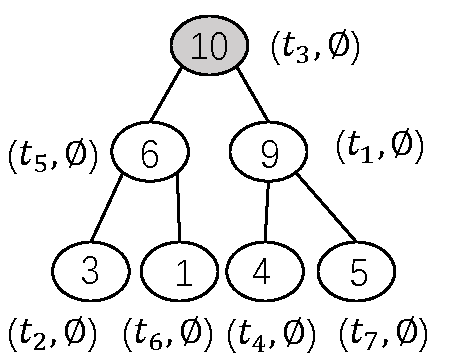
\includegraphics[width=0.4\columnwidth]{pictures/1st}
		&
		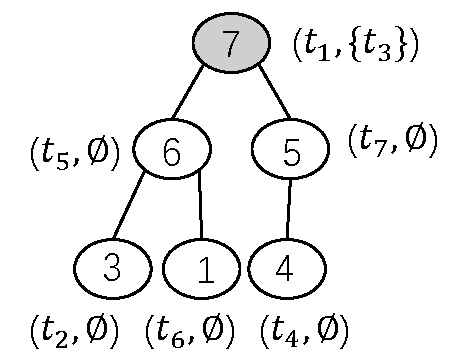
\includegraphics[width=0.4\columnwidth]{pictures/2nd}
		\\
		(A) 1st iteration
		&
		(B) 2nd iteration
	\end{tabular}
    \trim
	\caption{Heap-based lazy computation.} \label{fig:heap} %via the submodularity in Lemma~\ref{lem:submodular}
    \trim \trim
\end{figure}


\stitle{Heap-based lazy Computation}
Algorithm~\ref{alg:greedy} essentially adds the trajectory that maximizes $\Delta(\oR, t) = |\VV(\oR \cup t)| - |\VV(\oR)|$ to $\oR$ in each iteration.
Lemma~\ref{lem:submodular} shows that the contribution of a trajectory (i.e., $\Delta(\oR, t)$) cannot increase when Algorithm~\ref{alg:greedy} runs for more iterations because $ \Delta(\oR^{'}, t) \le \Delta(\oR, t) $ for  $\oR \subset \oR^{'}$.
For example, the contribution of $t_1$ is $9$ at the first iteration (i.e., $\oR = \emptyset$), see Figure~\ref{fig:heap}(a).
Its contribution turns $7$ when $\oR = \{ t_3 \}$ at the second iteration, as shown in Figure~\ref{fig:heap}(b).
Based on this property, we can use  $\Delta(\oR, t)$ calculated in the previous iterations to prune it from contribution computation.
Specifically, if we have $\Delta(\oR, t) \le \Delta(\oR^{'}, t')$, in which $\oR$ and $\oR^{'}$ are a previous and the current sample set, respectively,
we know that $t$ can not be added to the sample set in the current iteration as $\Delta(\oR^{'}, t)\le \Delta(\oR^{'}, t')$ and $t'$ is a better choice.
As shown in Figure~\ref{fig:heap}(b), even we do not know $\Delta(\oR'=\{t_3\}, t_7)$ exactly,
we can conclude $t_7$ will not be the sample set in the second iteration as $\Delta(\oR = \emptyset, t_7) = 5 < \Delta(\oR'=\{t_3\}, t_1) = 7$.


To implement this idea, we maintain a max-heap for the number of uncovered pixels in each trajectory and update the contribution of a trajectory only when necessary, i.e., computing in a lazy manner.

Consider a tiny example with 7 trajectories, i.e., $t_1$ to $t_7$.
Figure~\ref{fig:heap}(a) shows the initial max-heap and the contributions of trajectories $t_1$ to $t_7$ w.r.t result set $\oR = \emptyset$.
At the first iteration, the root node of the max-heap, $t_3$ in Figure~\ref{fig:heap}(A), is selected.
At the second iteration, the number of uncovered pixels of the new root node $t_1$ is updated to 7 w.r.t. result set $\oR = \{ t_3 \}$ (see the gray node in Figure~\ref{fig:heap}(B)).
Then $t_1$ is selected at the second iteration without computing the contributions of other trajectories w.r.t $\oR = \{ t_3 \}$.
The reason is that the contributions of these trajectories are all less than 7 when $\oR = \emptyset$,
according to the submodularity in Lemma~\ref{lem:submodular}, their contributions must be smaller than $7$ when $\oR = \{ t_3 \}$.
The efficiency of Algorithm~\ref{alg:greedy} is significantly improved with heap-based lazy computation.
Recall that Algorithm~\ref{alg:greedy} takes 413.6 seconds with sampling rate $0.1\%$ on the \pt{} dataset while our performance-optimized $\vats$ needs only 1.2 seconds.

%In summary, the number of uncovered pixels in each trajectory will only be computed with the latest result set $\oR$ when it is necessary in the lazy computing manner,
%e.g., only $t_1$ will be updated at the 2nd iteration in Figure~\ref{fig:heap}.
%It reduces many unnecessary computations through the lazy updating manner, e.g., all white nodes did not update at the 2nd iteration in the above example.

%We then analyze the time complexity of Algorithm~\ref{alg:greedy} with lazy computing manner in Theorem~\ref{lem:lazy}.
%
%\begin{lemma}[Optimized Time Complexity]~\label{lem:lazy}
%Given trajectory dataset $\D$ and an integer $k= \alpha |\D|$, the time complexity of Algorithm~\ref{alg:greedy} with lazy computing manner is $O(\alpha \cdot m \cdot x |\D| \log |\D|)$, where $x$ is the number of contribution computations among all $k$ iterations and $x \ll |\D|$.
%\end{lemma}
%
%\begin{proof}
%It first takes $O(|\D|)$ time to construct the max-heap~\cite{cormen2009introduction}.
%It incurs $O( m \cdot x \log |\D|)$ cost to select the trajectory with maximum uncovered pixels at each iteration ($k$ iterations in total).
%Hence, the overall cost is $O(|\D| + k \cdot m \cdot t \log |\D|)$.
%\end{proof}

\subsection{Advanced Approach $\vatss$}\label{subsec:VQGS+}

\begin{figure*}
   \begin{minipage}{0.7\textwidth}
     \centering
     \begin{tabular}{ccc}
     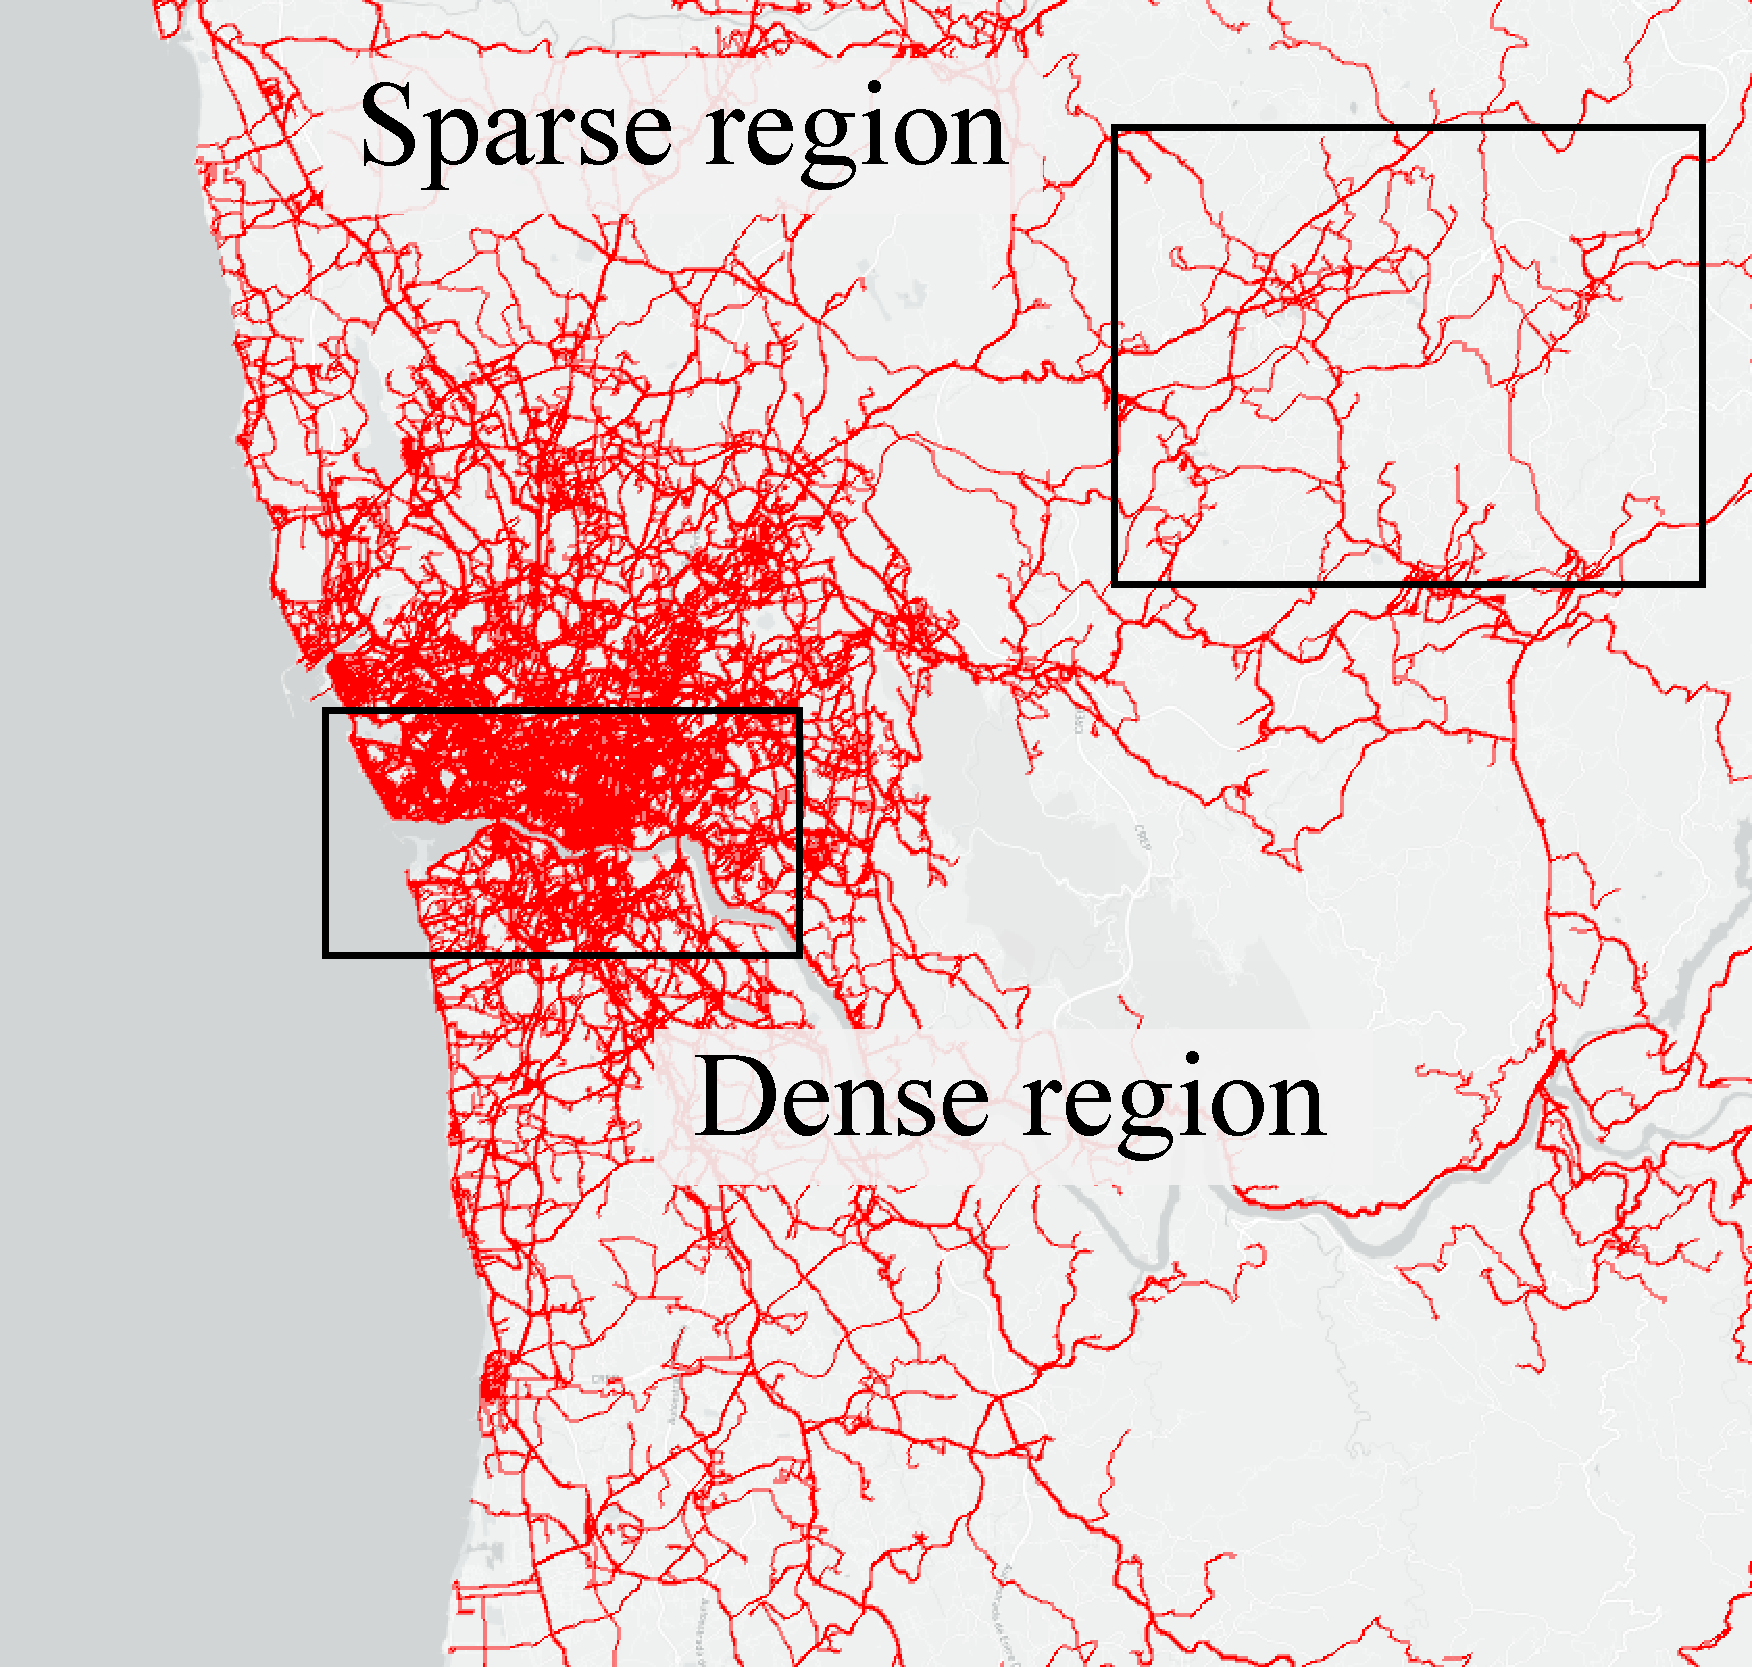
\includegraphics[width=0.250\linewidth]{pictures/motivation_VQGS}
     &
     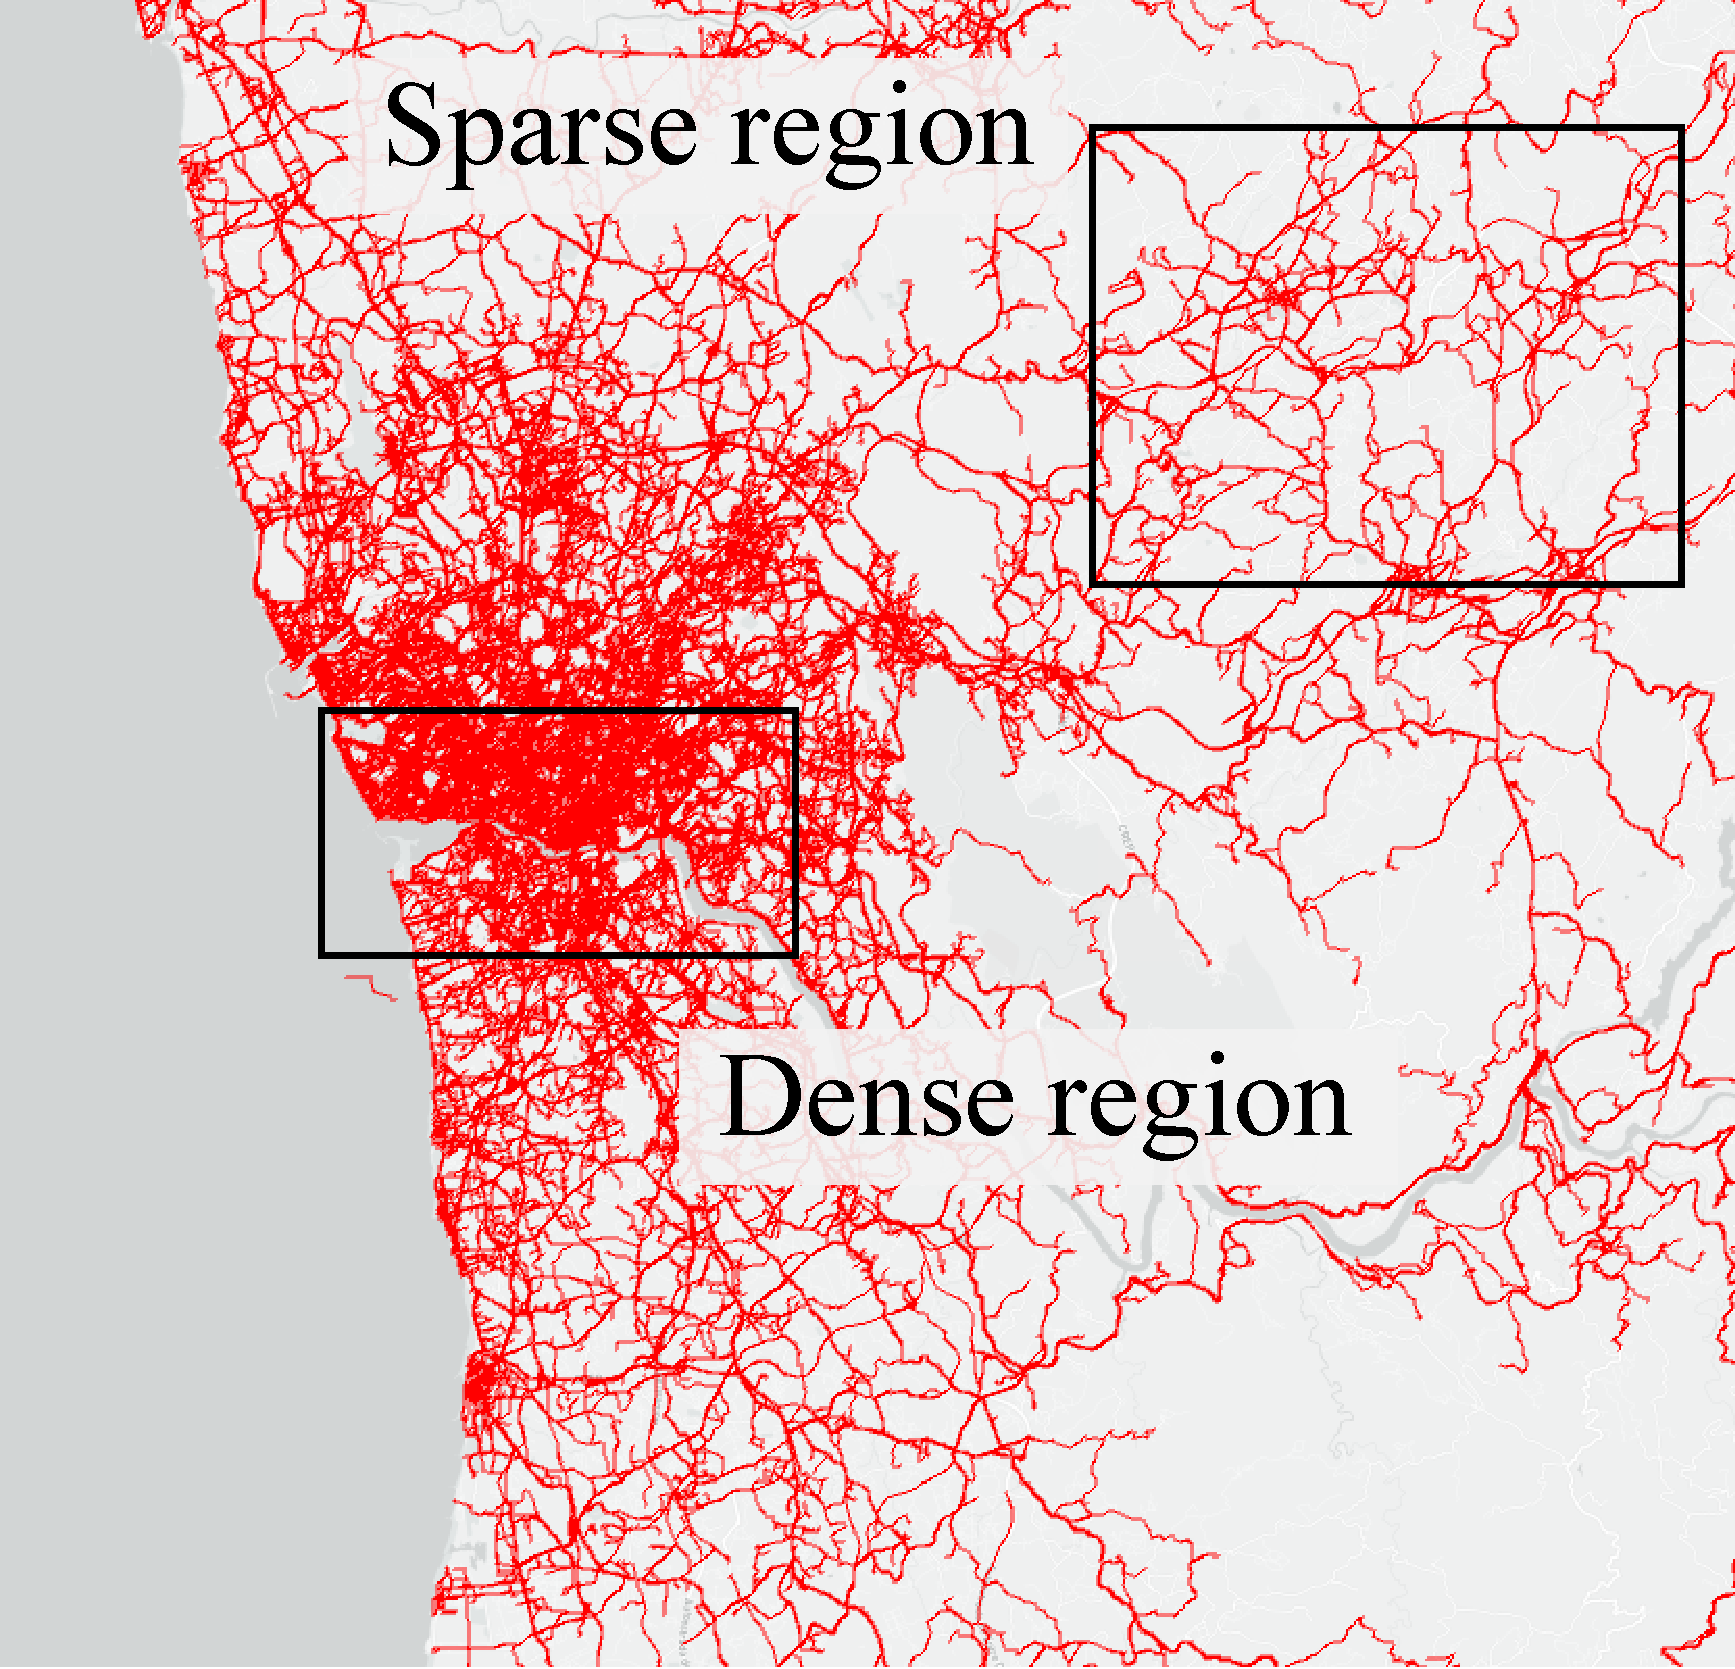
\includegraphics[width=0.250\linewidth]{pictures/motivation_VQGS+d64}
     &
     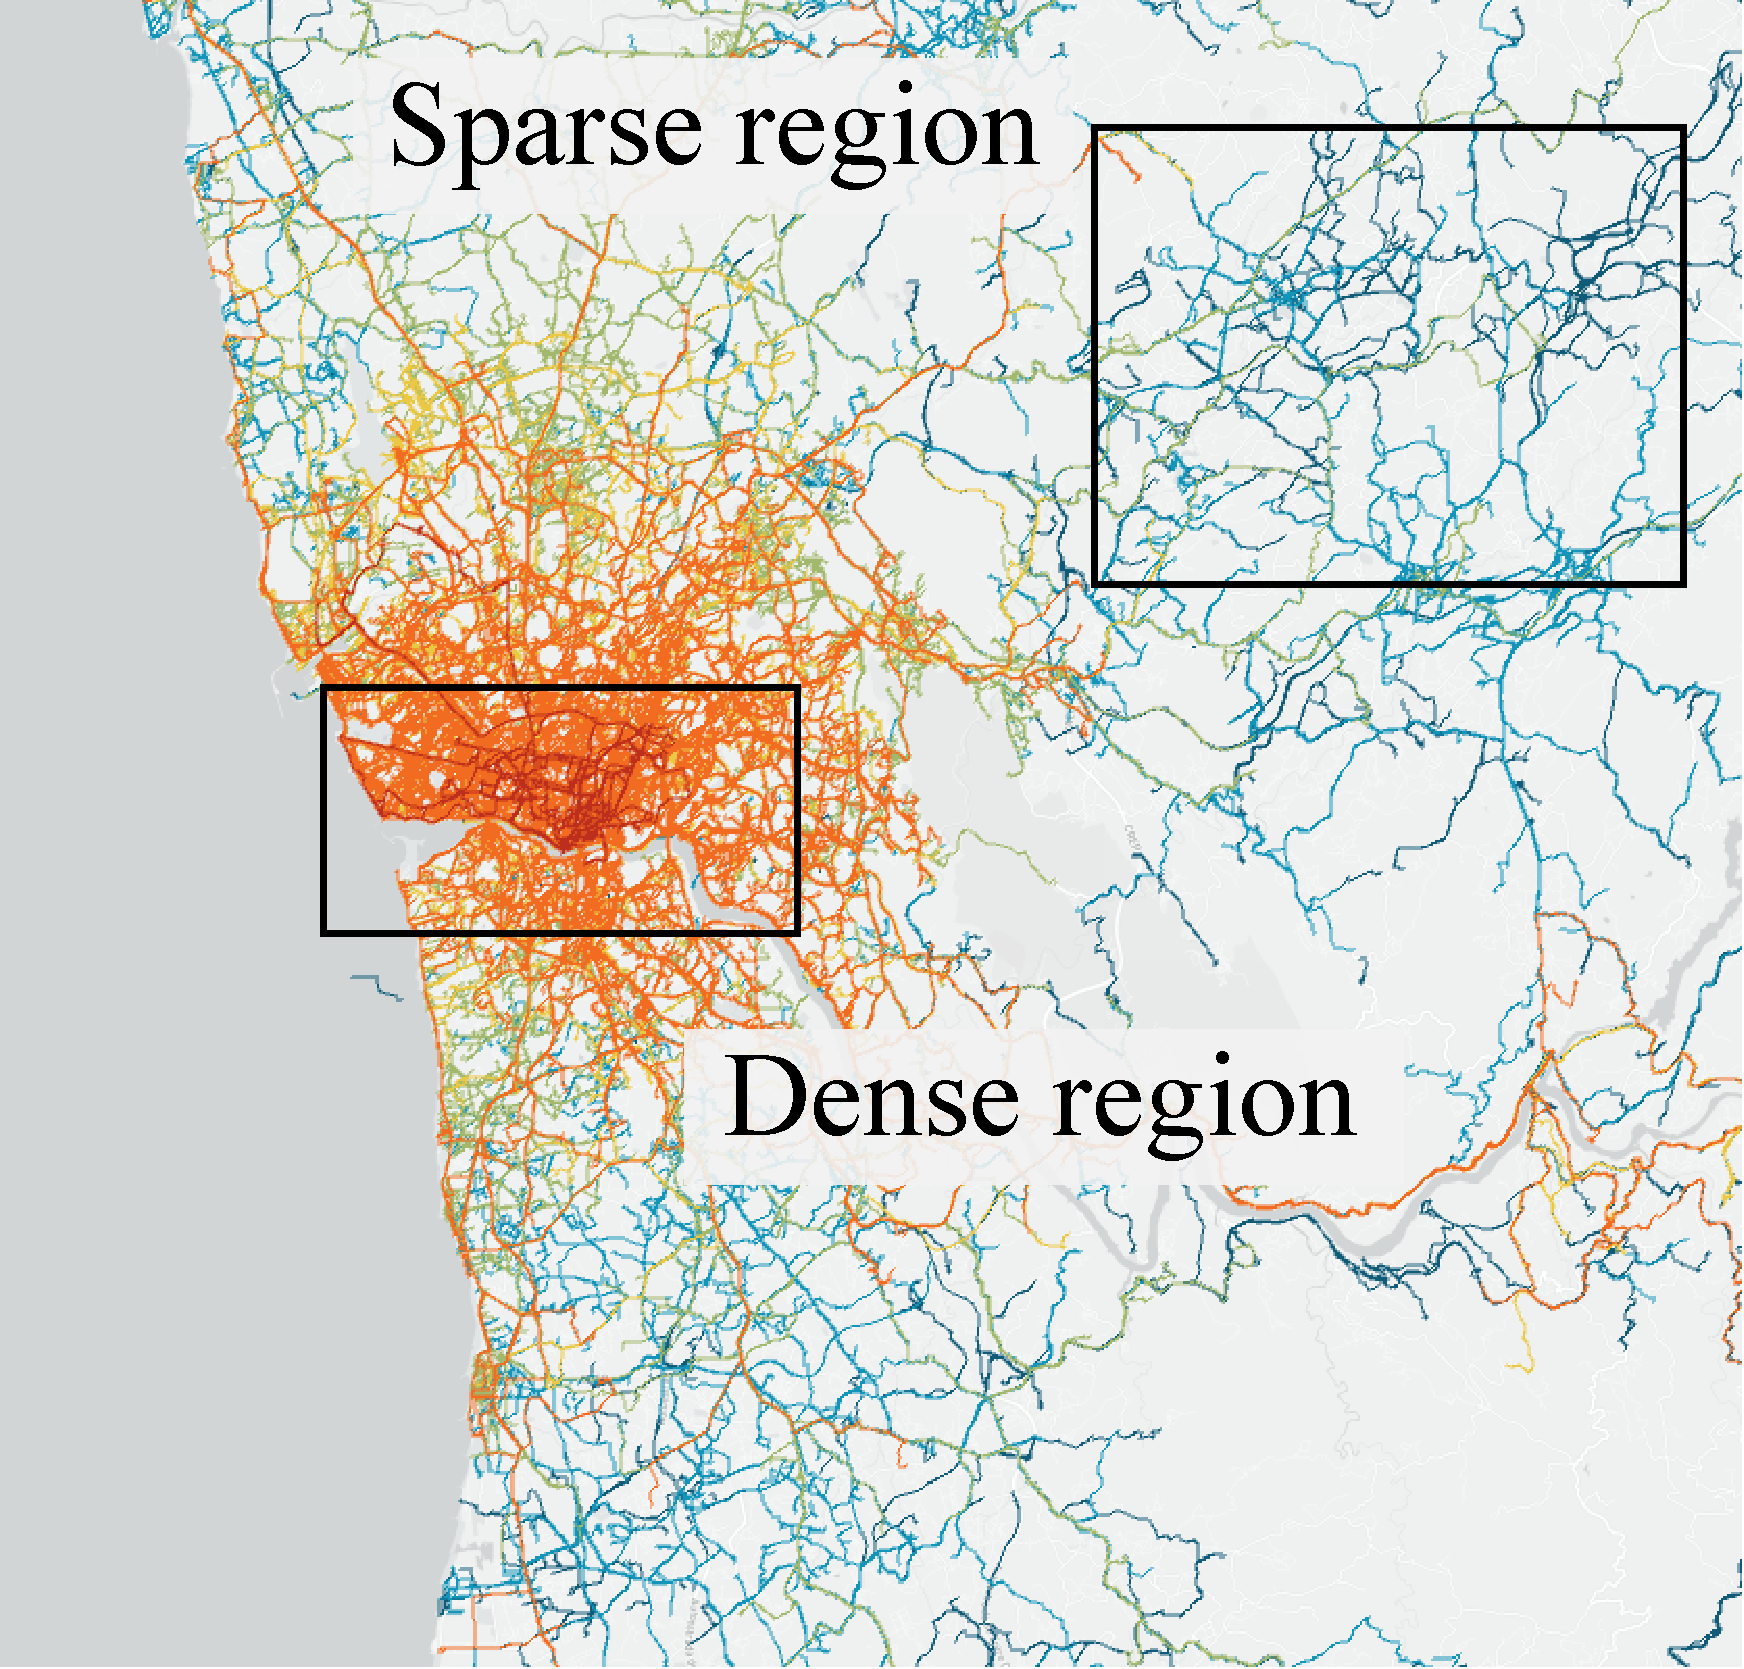
\includegraphics[width=0.250\linewidth]{pictures/motivation_VQGS+d64CE}
     \\
     (A) $\vats$
     &
     (B) $\vatss$
     &
     (C) $\vatssce$
     \end{tabular}
     \trim
     \caption{\prob{} solution $\vatss$ on \pt{} ($\alpha = 0.5\%, \delta = 64$)}\label{fig:delta}
   \end{minipage}\hfill
   \begin{minipage}{0.3\textwidth}
     \centering
     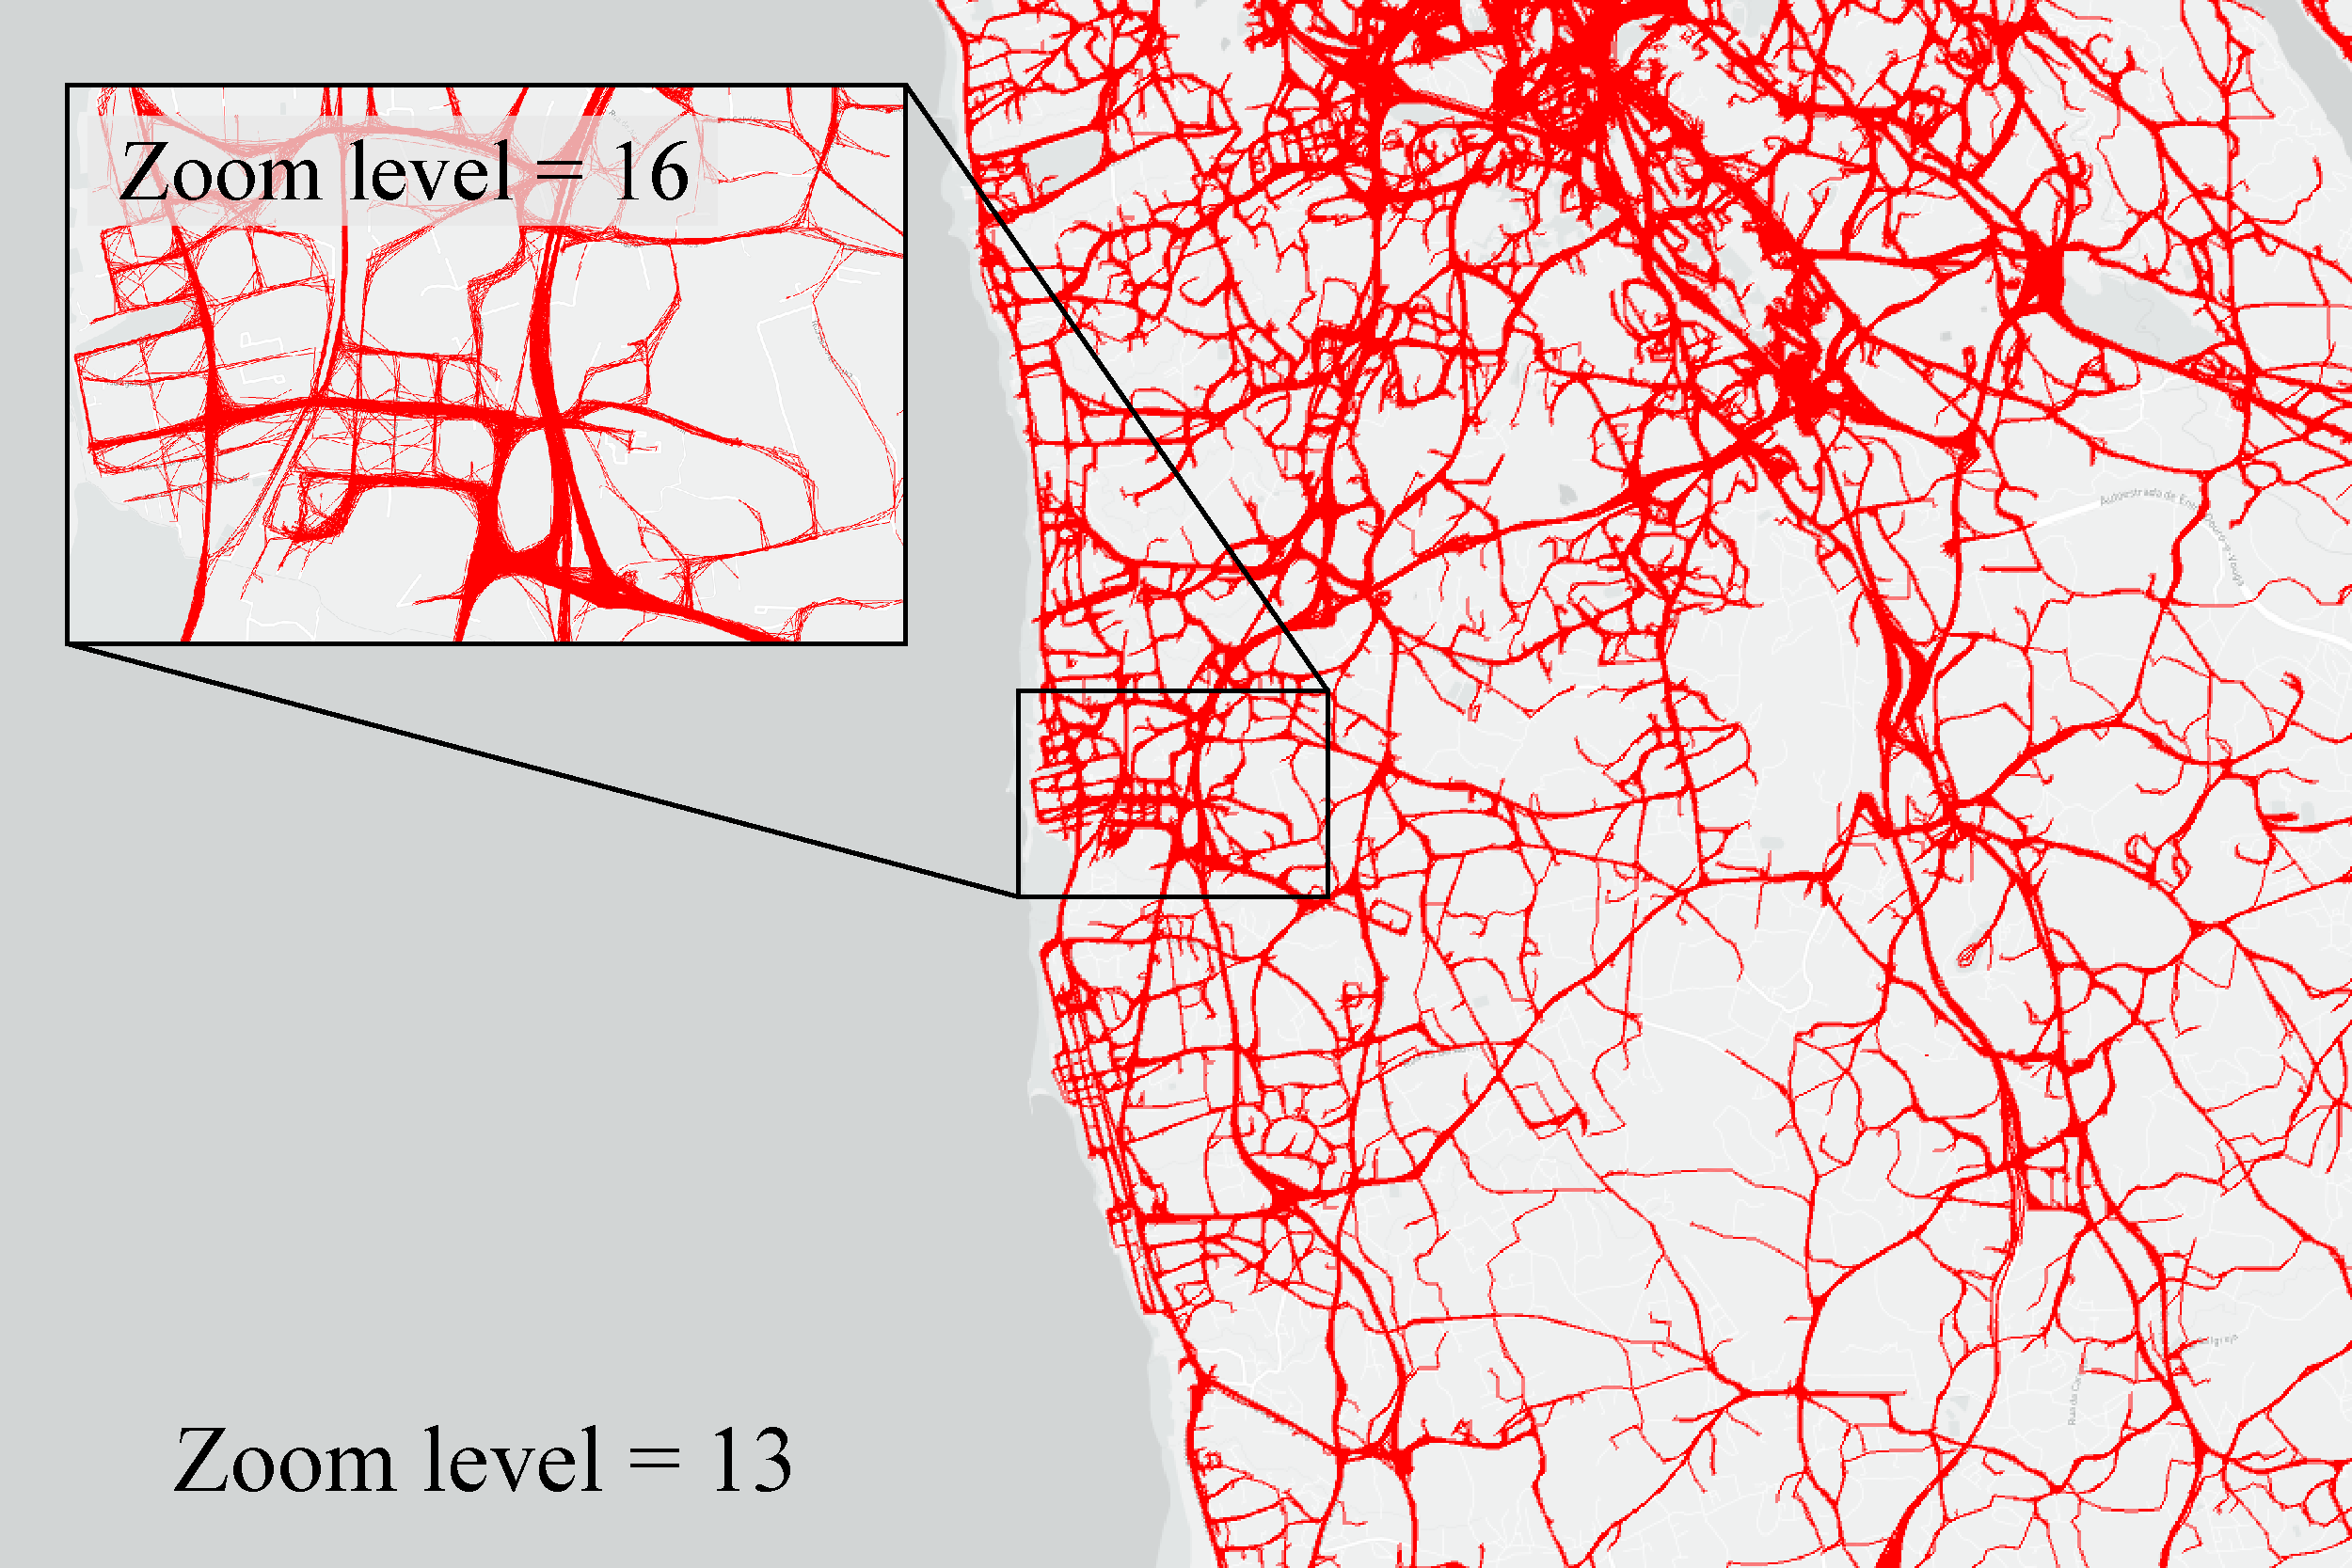
\includegraphics[width=0.85\linewidth]{pictures/zoomlevel.pdf}
     \label{Fig:zoom}
     \trim
     \caption{An illustration of different zoom level.}
   \end{minipage}
   \trim
\end{figure*}


%In the previous section, we presented the $\vats$ algorithm, which produces quality-guaranteed samples and runs efficiently. In this section, we focus on the third technical challenge: \emph{how to tackle the visual clutter problem in large trajectory visualization}?

In this part, we improve $\vats$ by considering (i) trajectory data distribution, and (ii) human perception capability. We elaborate (i) and (ii) by the examples in Figure~\ref{fig:delta}.


\stitle{Trajectory data distribution} Considering the \pt{} trajectory dataset, Figure~\ref{fig:delta}(A) is the visualization result of $\vats$ with sampling rate $0.5\%$.
It is obvious that the trajectories follow a non-uniform distribution, and there are some dense regions and sparse regions as illustrated by the two rectangles in Figure~\ref{fig:delta}(A).
There are many points in the dense region, which creates visual clutter and makes it difficult to identify the main roads.


%Obviously, the real-world trajectory dataset is non-uniform distributed.
%For example, the trajectories in dense region are much more than those in the sparse region, as illustrated by the rectangles in Figure~\ref{fig:delta}(A).

\stitle{Human perception capability} Comparing Figures~\ref{fig:delta}(A) and (B), it is easier to tell their differences in the sparse regions than in the dense regions.
This is because human perception has limited capability, and hence two visualizations look indistinguishable if both of them contain a large number of points in the same area.
The two dense regions look similar although Figure~\ref{fig:delta}(B) contain fewer points in this region than Figure~\ref{fig:delta}(A).
However, for the sparse region, $\vats$ loses some trajectories and it is easy to tell the differences between Figures~\ref{fig:delta}(A) and~\ref{fig:delta}(B).

%\begin{figure*}%[t]
%    \centering
%	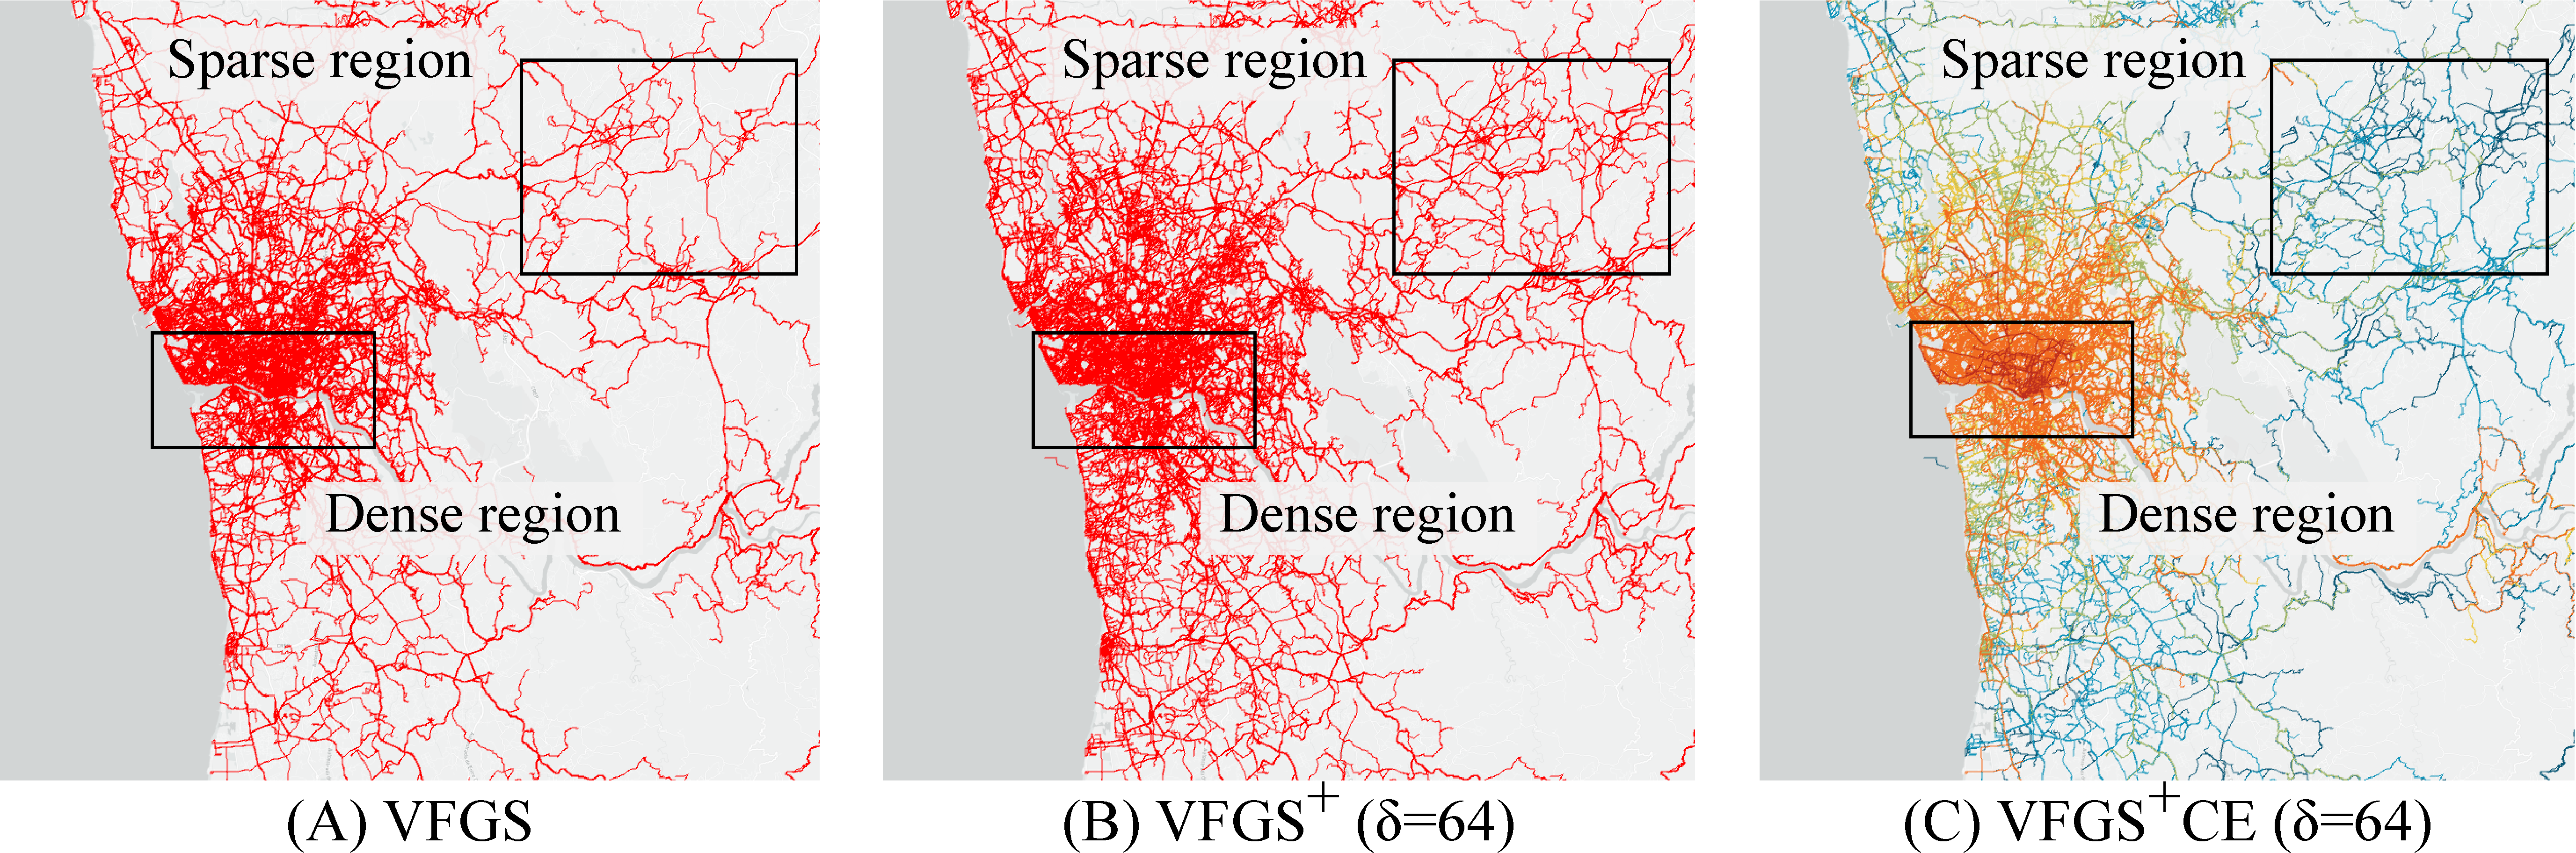
\includegraphics[width=0.7\textwidth]{pictures/problemsolveing/delta_motivation.pdf}
%	\caption{The advanced approach $\vatss$ on \pt{} ($\alpha = 0.5\%$).\Bo{edit figure captions}}\label{fig:delta}
%\end{figure*}


%\begin{table}
%  \begin{tabular}{cc}
%        \begin{figure}%[t]
%	       \centering
%	       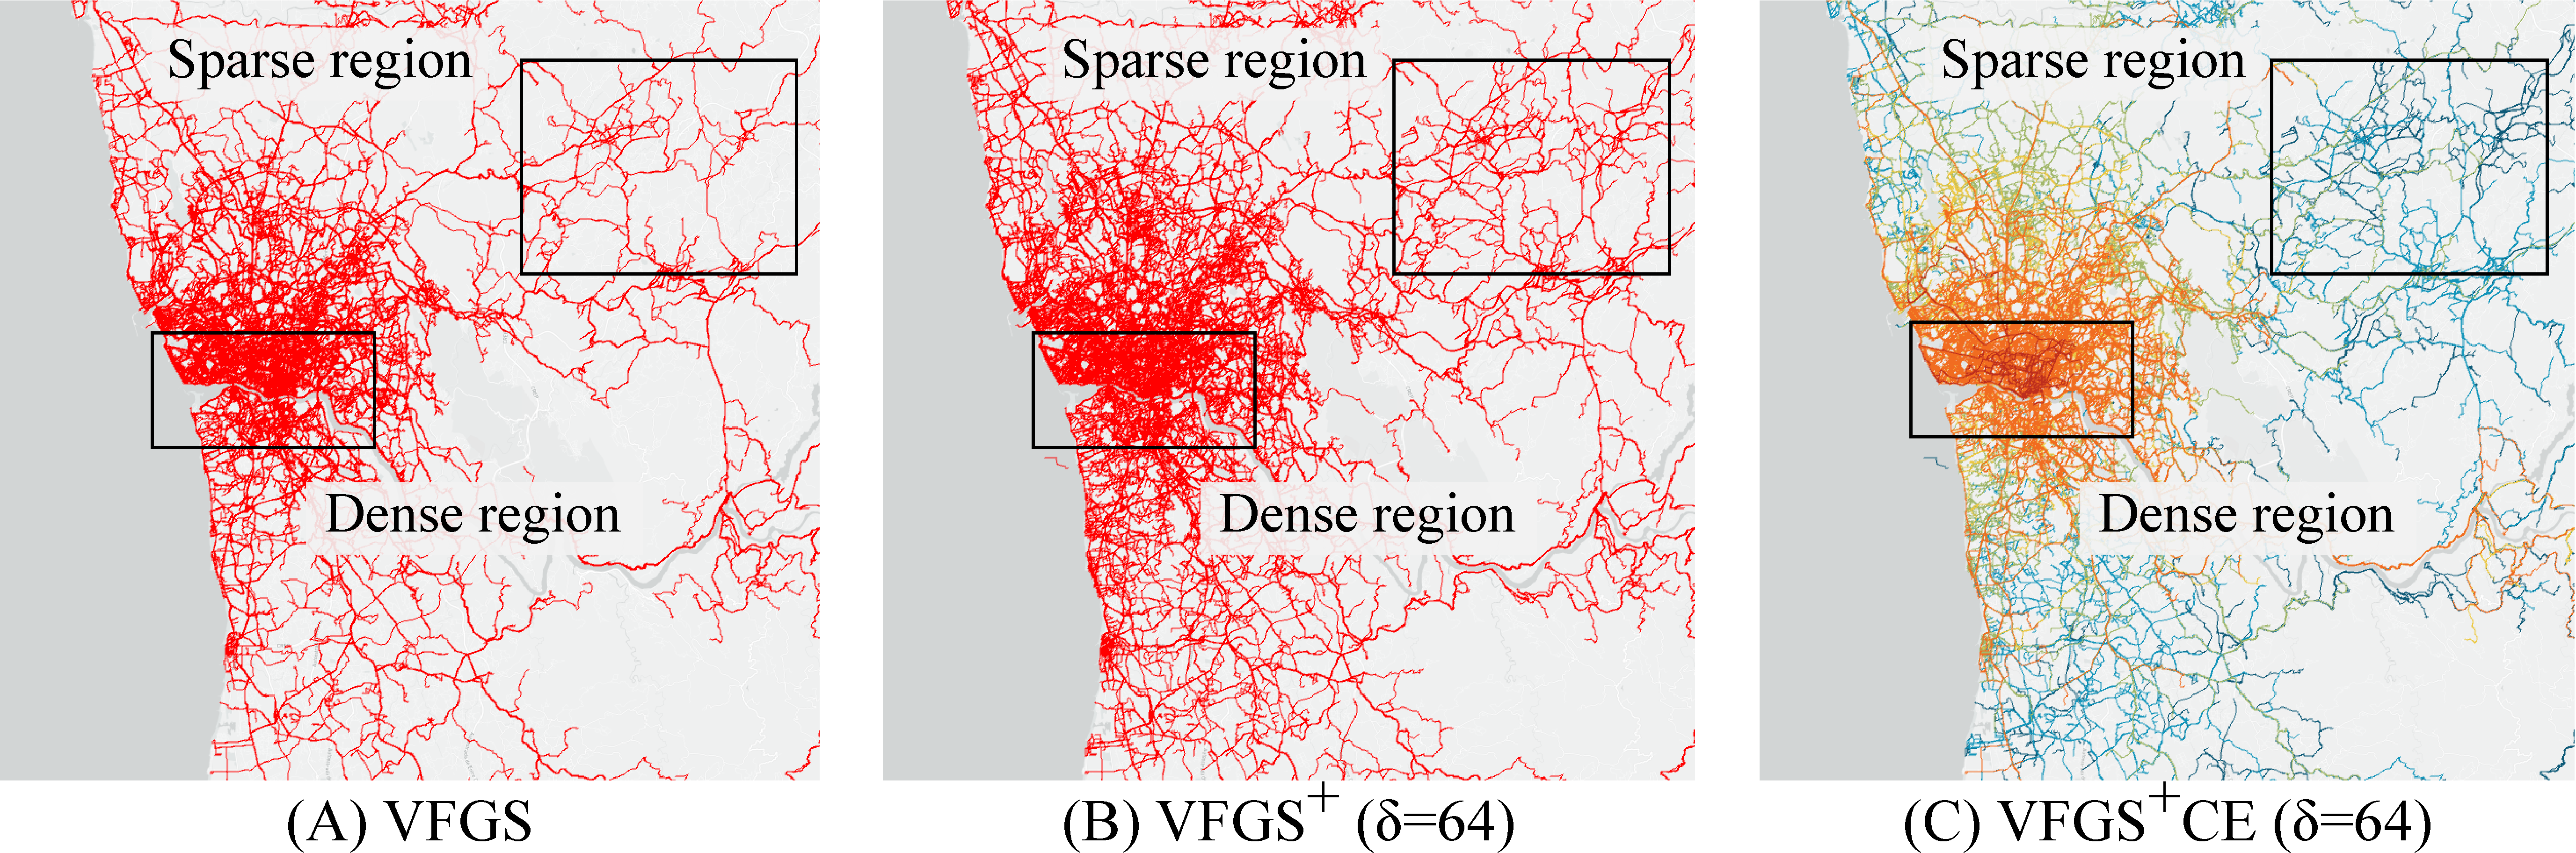
\includegraphics[width=0.7\textwidth]{pictures/problemsolveing/delta_motivation.pdf}
%	       \caption{The advanced approach $\vatss$ on \pt{} ($\alpha = 0.5\%$).\Bo{edit figure captions}}\label{fig:delta}
%        \end{figure}
%      &
%        \begin{figure}[t]
%        	\centering
%        	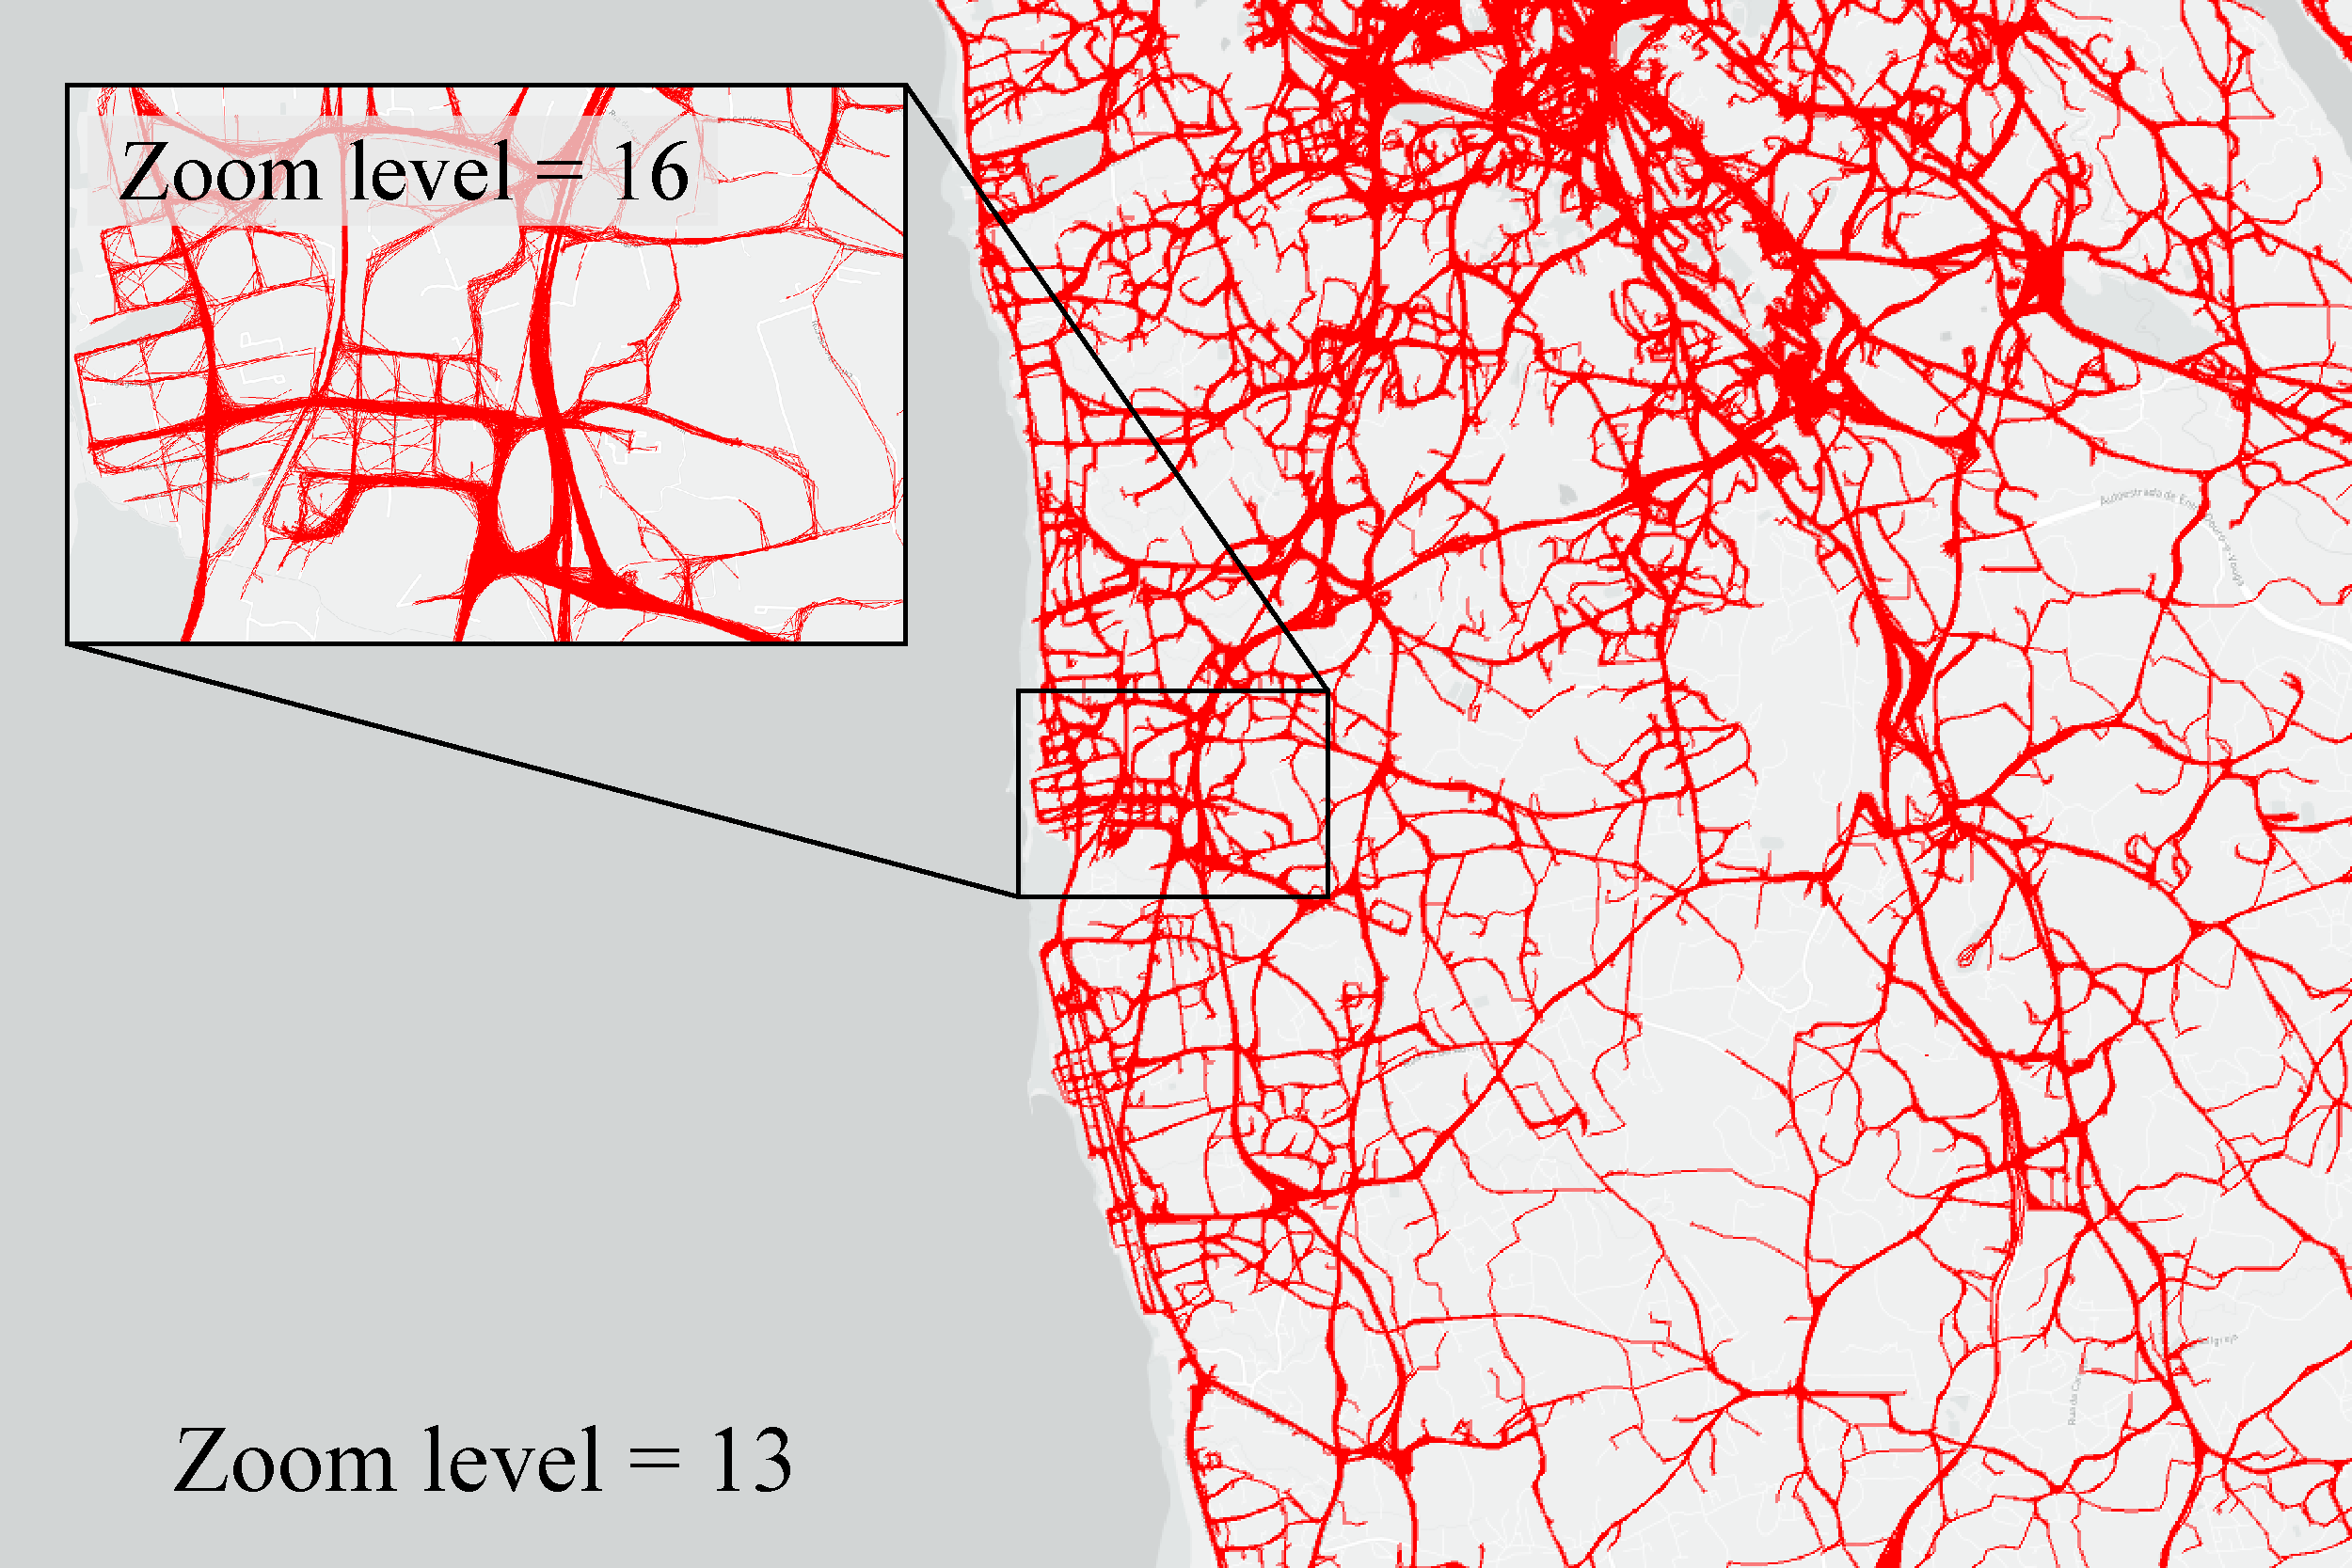
\includegraphics[width=0.3\textwidth]{pictures/zoomlevel.pdf}
%        	\caption{An illustration of different zoom level.}	\label{fig:zoom}
%        \end{figure}
%  \end{tabular}
%\end{table}



%(see Algorithm~\ref{alg:plus})

Based on the two observations above, we can improve  $\vats$ by delivering richer information in the sparse regions and reducing visual clutter in the dense regions.
$\vatss$ in Algorithm~\ref{alg:plus} achieves both objectives using a perception tolerance parameter $\delta$, which models the perception capability of humans.
Specifically, if pixel $(x,y)$ in the canvas is marked by the result set $\oR$,
the pixels around $(x,y)$, i.e., from $(x-\delta, y-\delta)$ to $(x+\delta, y+\delta)$, do not need to be marked as they are close to the pixels in $\oR$ and human perception cannot tell nearby pixels apart. We can easily modify $\vats$ in Algorithm~\ref{alg:greedy} to incorporate the perception tolerance parameter $\delta$ as shown in Algorithm~\ref{alg:plus}.
$\vatss$ measures the contribution of each trajectory $t_i$ w.r.t the augmented visualized point set $\VV(\oR)^{+}$ in Line~\ref{line:deltamax},
where $\VV(\oR)^{+}$ includes both pixels on the selected trajectories and their tolerance pixels (in Line~\ref{line:delta}).
We also use the heap-based lazy computation to speedup $\vatss$.


%Taking the above two observations into consideration, we can further improve the returning result of visual quality-guaranteed sampling approach $\vats$ by
%delivering rich information at sparse regions and reducing visual clutter in dense regions.
%In this section, we devise the advanced approach $\avats$ (see Algorithm~\ref{alg:plus}) to achieve the above two objectives.
%In specific, we introduce perception tolerance parameter $\delta$ in $\avats$, which models the perception capability of humans at the highest level of details.
%In other words, suppose the pixel $(x,y)$ in canvas is covered by the result set $\oR$ at the highest level,
%the pixels around $(x,y)$, i.e., from $(x-\delta, y-\delta)$ to $(x+\delta, y+\delta)$, are not necessary to cover because they are in the perception tolerance of human beings.


%It measures the contribution of each trajectory $t_i$ w.r.t the selected trajectory set $\oR$'s augmented set $\oR^{+}$, i.e., the selected trajectories and their tolerance pixels.
%.
%The augmented set $\oR^{+}$ will be updated by the selected trajectory $tmp$ and its tolerance pixels set (in Line~\ref{line:delta}).

%
\begin{algorithm}
    \caption{$\vatss(\D,k=\lceil \alpha \mathcal{T} \rceil,\delta)$} \label{alg:plus}
    \begin{algorithmic}[1]
    \State Initialize result set $\oR \leftarrow \emptyset$
    \State Initialize augmented result set $\oR^{+} \leftarrow \emptyset$
    \While{$|\oR| < k$}
        \State $\mathsf{tmp} \leftarrow \arg\max_{t_i \in \D} | t_i  \cup \VV(\oR)^{+} |$ \label{line:deltamax}
        \State $\oR \leftarrow \oR \cup \{ \mathsf{tmp} \}$
        \State $\VV(\oR)^{+} \leftarrow \VV(\oR)^{+} \cup \mathsf{augment}(\mathsf{tmp}, \delta)$\label{line:delta}
    \EndWhile
    \For{each $t$ in $\D$} \Comment{Representative encoding} \label{line:s}
        \State $tr \leftarrow \arg\min_{t_i \in \oR}{|t-\mathsf{augment}(t_i, \delta)|}$
        \State $tr.\mathsf{cnt}++$ \label{line:e}
    \EndFor
    \State Return $\oR$
    \end{algorithmic}
\end{algorithm}


%Interestingly, the visual clutter large trajectory visualization problem can be further reduced
%by encoding representative trajectories in $\oR$ (the returning result of $\avats$) with colors.
%In particular, $\avats$ selects the trajectory with the largest uncovered pixels by taking the perception tolerance capability of humans into account at each iteration,
%instead of only choosing the trajectory with the largest uncovered pixels in $\vats$ (Algorithm~\ref{alg:greedy}).


$\vatss$ in Algorithm~\ref{alg:plus} selects trajectories with good representativeness and some trajectories will not be included into the result set $\oR$ even though they have more uncovered pixels w.r.t. $\oR$.
The reason is that their uncovered pixels are too close to the pixels in the selected trajectories (i.e., within the tolerance area of selected pixels).
Compared with $\vats$, $\vatss$ is more likely to sample trajectories in the sparse regions as their pixels are less likely to be covered by other trajectories as shown in Figures~\ref{fig:delta}.
Moreover, reducing the number of trajectories sampled from the dense regions helps to reduce visual clutter.


%Take Figure~\ref{fig:zoom}(A) for example, suppose $\delta=1$ and trajectory $a$ was selected at the first iteration, the trajectory to select in the second iteration is $c$ instead of $b$ because almost all pixels in $b$ is in the tolerance area of $a$'s.

%\begin{figure}[t]
%	\centering
%	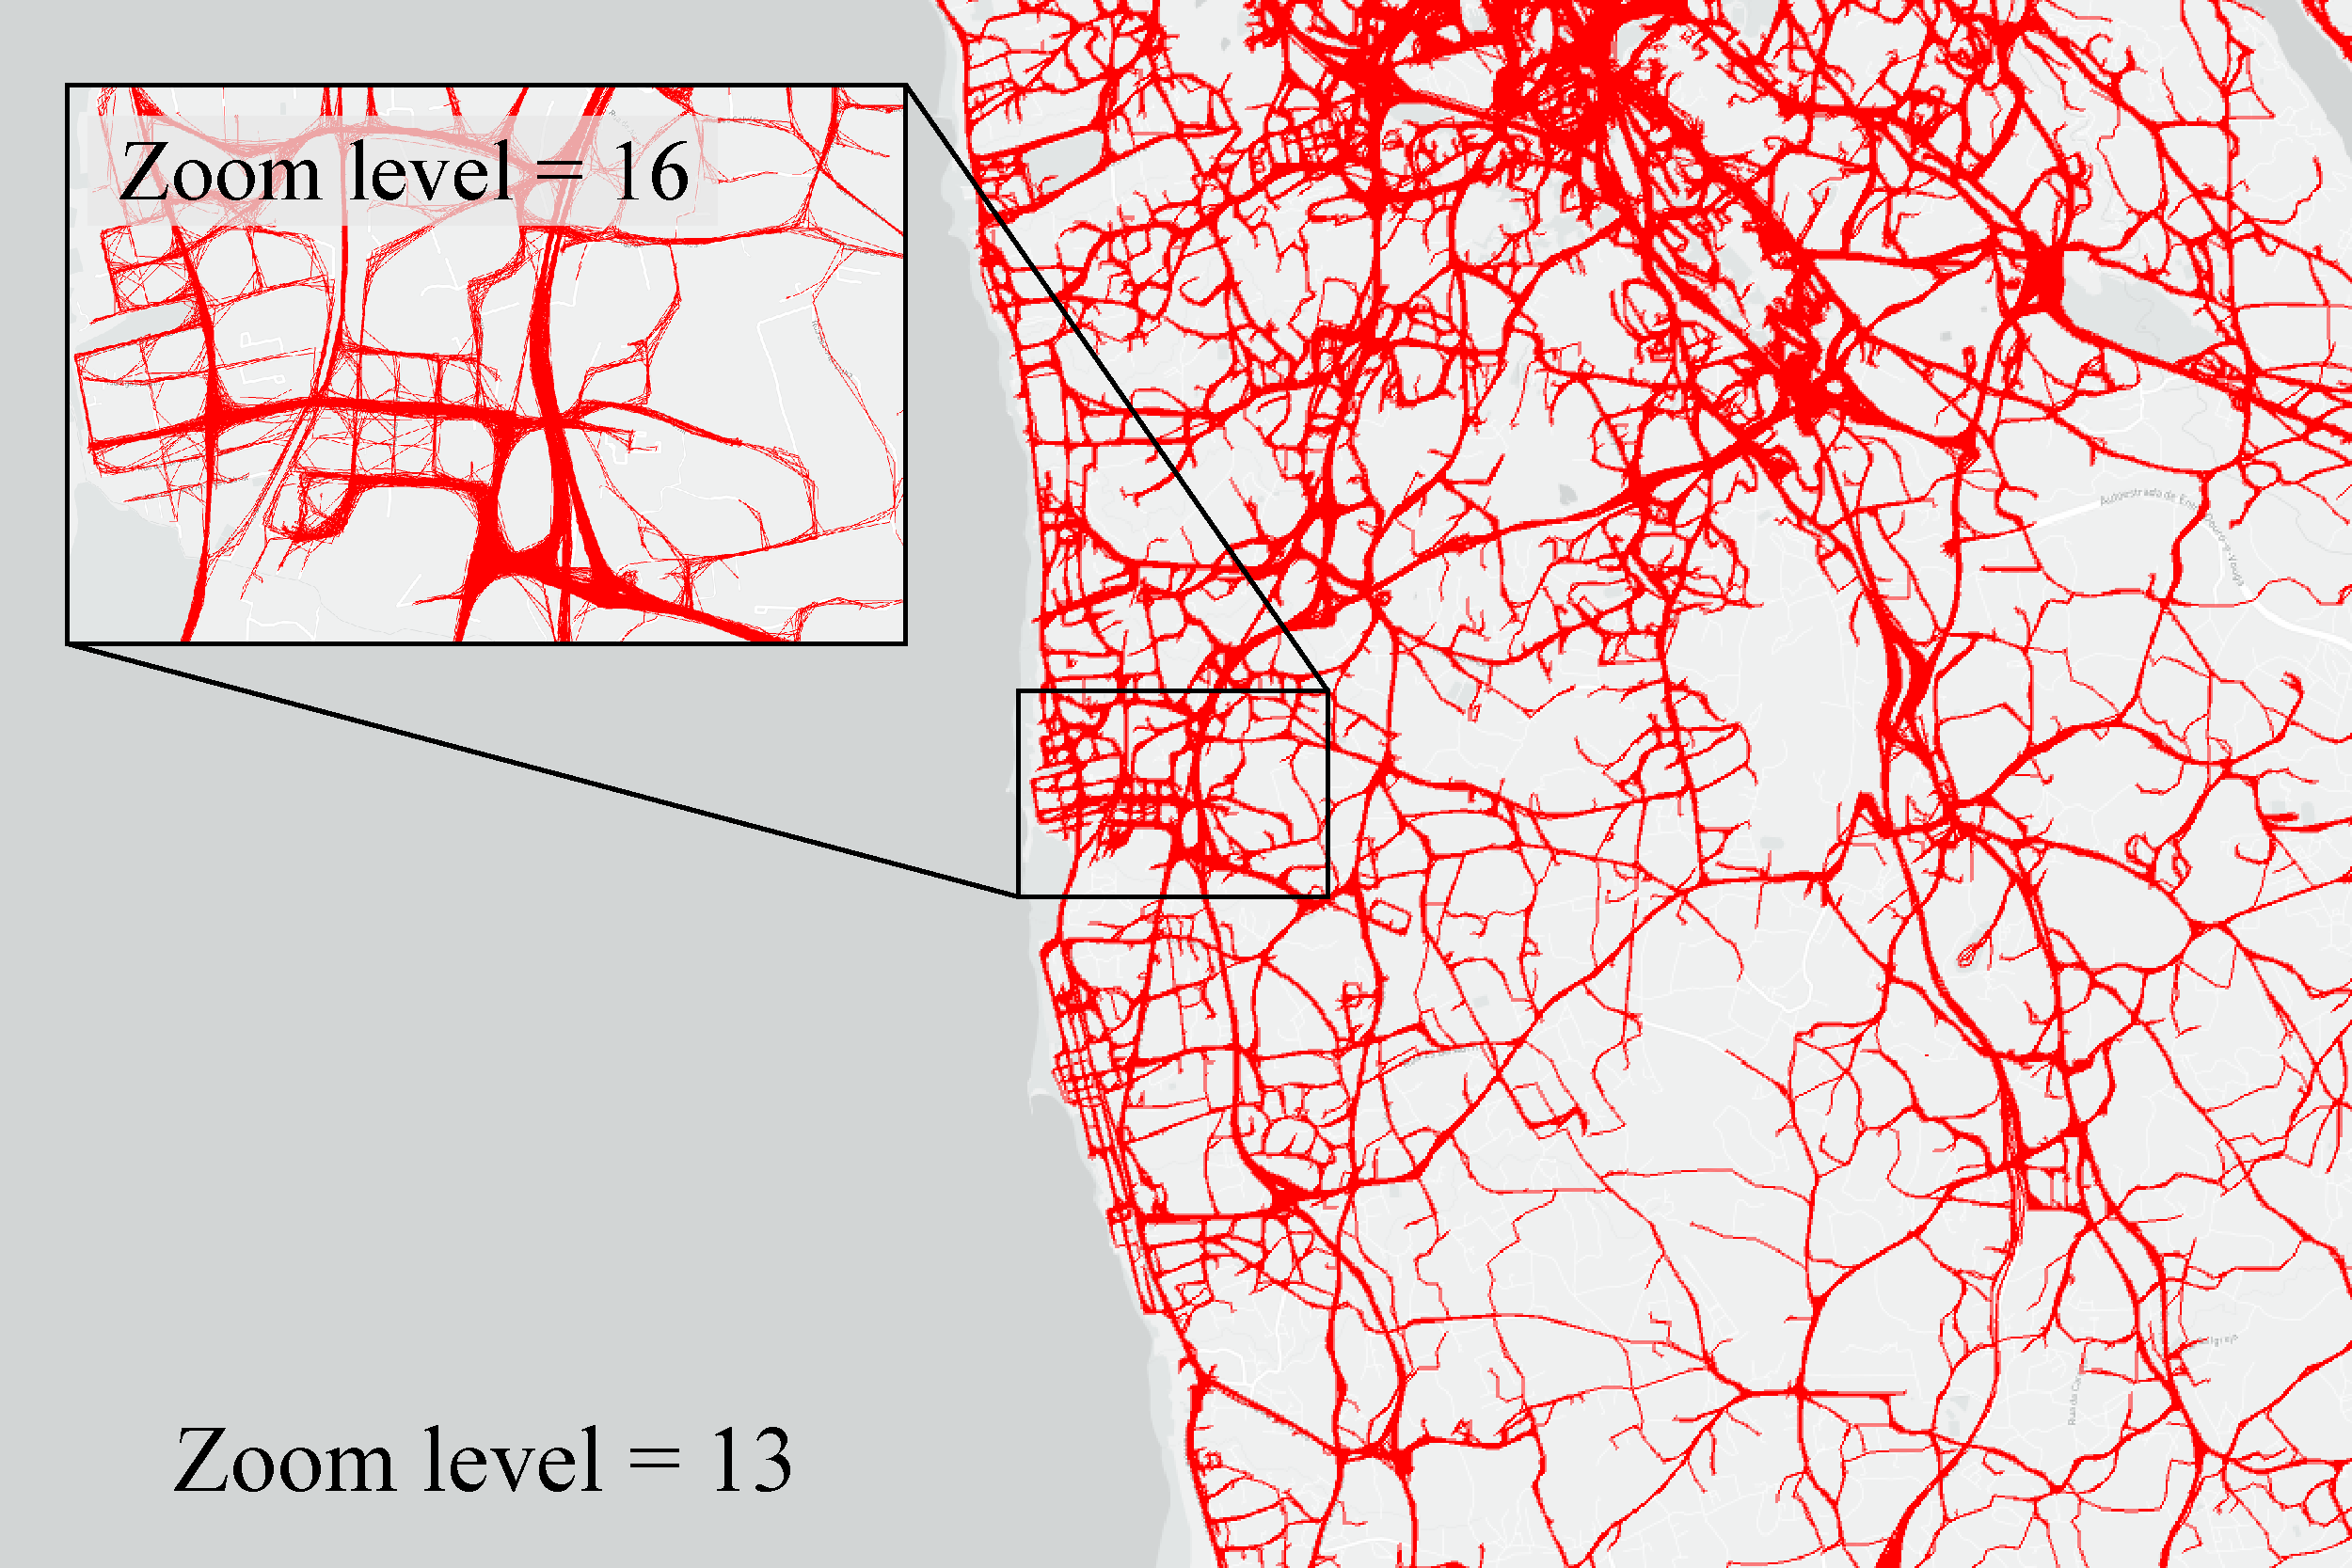
\includegraphics[width=0.3\textwidth]{pictures/zoomlevel.pdf}
%	\caption{An illustration of different zoom level.}	\label{fig:zoom}
%\end{figure}


One subtlety is that different $\delta$ needs to used for different \emph{zoom levels} (or regions with different sizes).
For example, Google map~\cite{googlemap} provides zoom levels from 0 to 20, with level 0 providing the largest visualization range (i.e., the whole world) but the lowest resolution, and level 20 providing the smallest visualization range (e.g., individual building, if available) but the highest resolution.
We provided an illustration of zoom level in Figure 6 and users may select different zoom levels for visualization according their needs.
Note that we define $\delta$ on the highest zoom level (i.e., using the raw distance of the locations) to account for different resolutions.
If the zoom level is small (i.e., the visualization region is large), we can apply a large $\delta$ because locations with a large raw distance look close to each other in the visualization and we can afford to lose more details.
If the zoom level is large (i.e., the visualization region is small), we need to use a small $\delta$ as users typically want to investigate some fine-grained details in this case and using a large $\delta$ will lose these details.

%We will elaborate this point shortly in experimental section.

%Therefore, we use different $\delta$ for different zoom levels accordion to Table~\ref{tab:delta}, which was obtained empirically from a user evaluation of the visualization results.
%\begin{table}
%	\centering
%	\small
%	\caption{Values of $\delta$ for different zoom levels}
%	\begin{tabular}{|c|c|c|c|c|} \hline
%		\textbf{Zoom Level} &  &  &  & \\
%		\hline
%		$\delta$ &  &  & &  \\ \hline
%	\end{tabular}	\label{tab:delta}
%\end{table}

%Ideally, we want a sample to be \textit{zoom-level-independent}, providing a consistent quality guarantee at different zoom levels. This turns out to be straightforward as trajectory visualization merges several pixels in a high-level result (by pixel-wise $OR$) to obtain a pixel in a lower-level visualization result. The following theorem shows that it suffices to satisfy the quality guarantee at the highest zoom level.

%$\delta$ for different zoom levels, user study smaller delta for higher zoom levels


%$\vatss$ also provides excellent visual quality at arbitrary zooming resolutions. This is because it considers the perception tolerance parameter $\delta$  at the highest zoom level. For example, the zoom level in Figure~\ref{fig:zoom}(A) is higher than that in Figure~\ref{fig:zoom}(B). According to our elaboration, $\vatss$ selects trajectory $a$ and $c$ for Figure~\ref{fig:zoom}(A). When the area is zoomed out, as shown in Figure~\ref{fig:zoom}(B), trajectory $a$ and $c$ still captures the main sketch of the underlying dataset (as gray cells shown).





\stitle{Color encoding scheme}
The visual clutter problem for large-scale trajectory visualization can be further alleviated by encoding the representativeness of the trajectories in $\oR$ with colors.
We define the representativeness of a trajectory $t_i$ in $\oR$ as the size of its \emph{reverse nearest neighbor set}, which contains the trajectories in $\D$ that has $t_i$ as its nearest neighbor in $\oR$.
The distance between trajectory $t$ and $t_i$ is defined as the number of pixels in $t$ that can not be covered by the augmented pixels of $t_i$.
We compute the representativeness of each trajectory in $\oR$ in Lines~\ref{line:s}-\ref{line:e} in Algorithm~\ref{alg:plus}.
Figure~\ref{fig:delta}(C) shows the visualization result by encoding trajectories with larger representativeness with warmer colors. Compared with Figure~\ref{fig:delta}(B), the main roads in the dense region is clearer in Figure~\ref{fig:delta}(C) with very warm colors.

%There are more details in the sparse regions compared with the $\vats$ result in Figure~\ref{fig:delta}(A), and we can identify the main roads in the dense region with very warm colors.

%Thus, the selected trajectories in the dense region are more representative than those in sparse region.



%		&
%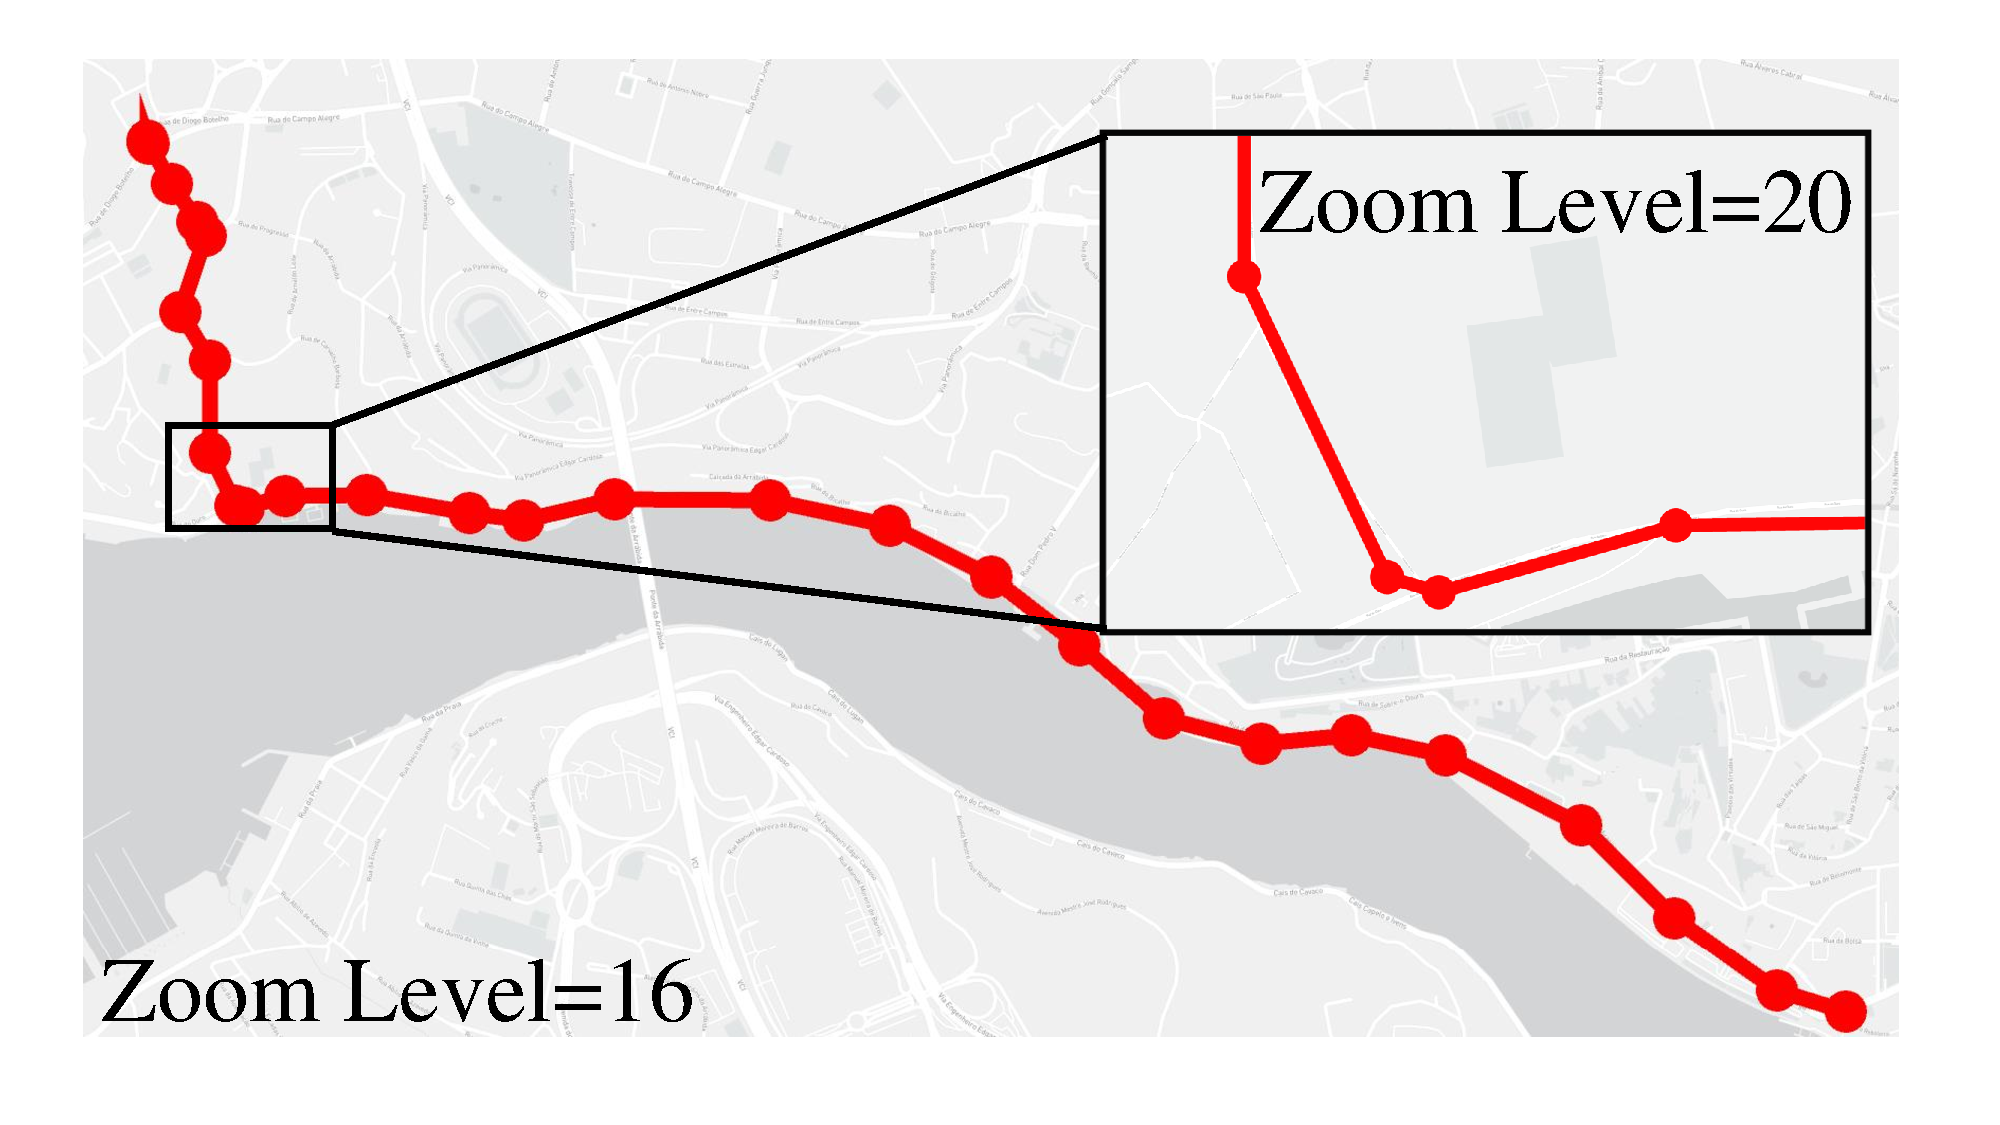
\includegraphics[width=0.48\columnwidth]{pictures/problemsolveing/TrajZoomIn}		
%\\
%(A) Line-based visualization
%&
%(B) Zoom levels


%(1) Richer Information Delivering: details aware; so Arbitrary zooming resolutions
%(2) Popularity Embedding: visual clutter



%\subsection{One-to-many strategy}~\label{sec:one_to_many}
%Since we detect the covered pixels in the highest level, two trajectories may be very close to each other but share very few pixels, which will lead to more information loss in the low zoom view as figure~\ref{fig:one_to_many}.
%We next elaborate a ``one-to-many'' strategy to further optimize the visual quality of our proposed technique.
%Recalling we use the highest zoom level to define the pixel size in the canvas.
%Thus, our visual quality guaranteed sampling algorithm is zoom-level oblivious, e.g., it guarantees the visual quality of result set $\oR$ at every zoom level.
%However, users always do not use/need the highest zoom level in visualization applications.
%For example, Google map shows city and streets at zoom level 1 and 15, respectively~\footnote{\url{https://developers.google.com/maps/documentation/}}.
%Motivated by the above observation, we devise ``one-to-many'' strategy by introducing a visual tolerance parameter $\delta$ to optimize the visual quality for users.
%Specifically, ,
%the ``one-to-many'' strategy will ignore all the pixels around $(x,y)$ within $\delta$ offset distance, i.e., all pixels from $(x-\delta, y-\delta)$ to $(x+\delta, y+\delta)$ will be skipped.
%We will demonstrate the effectiveness of the visual tolerance $\delta$ in experimental evaluations.
%
%%https://developers.google.com/maps/documentation/maps-static/dev-guide#Zoomlevels
%\begin{figure}[t]
%	\centering
%	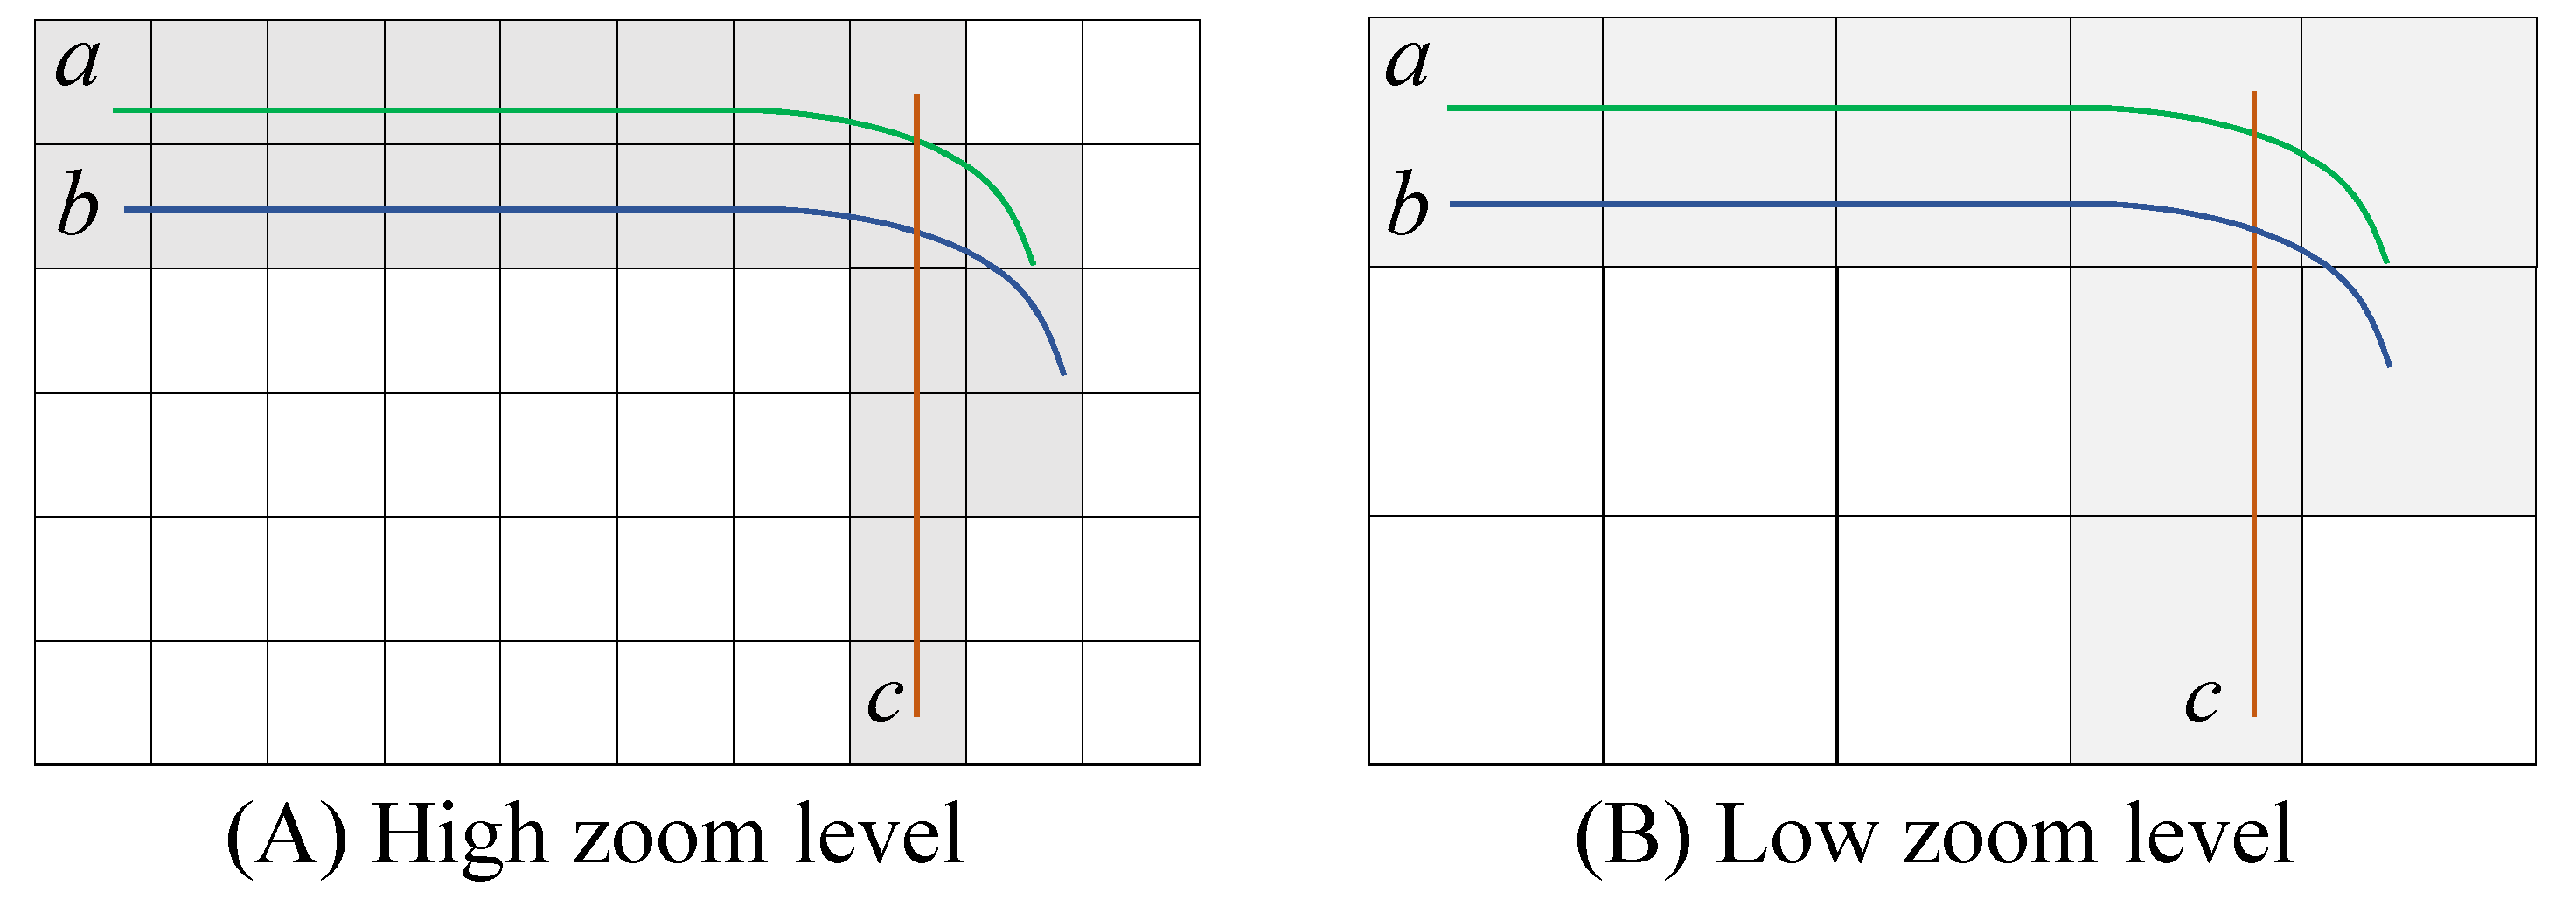
\includegraphics[width=0.4\textwidth]{pictures/problemsolveing/one_to_many.pdf}
%	\vspace{-5mm}
%	\caption{Resolution inconsistency}
%	\vspace{-5mm}
%	\label{fig:one_to_many}
%\end{figure}


%Specifically, $\avats$ incorporates a parameter $\delta$ during trajectory selection process in $\vats$ .
%In particular, we employ the parameter $\delta$ to model the end user's perception ability at the most high level of details.
%Surprisingly, our advance approach $\avats$ not only provides better visualization result when comparing with $\vats$ with the same sampling rate
%(e.g., Figure~\ref{fig:delta}(a) and (b) are the returning result of $\vats$ and $\avats$ respectively),
%but also embeds the popularity of selected trajectories by encoding the rest trajectories in the dataset in them,
%e.g., Figure~\ref{fig:delta}(c) is the visual result of $\avats$ with color encoded popularity.





\section{The $\avats$ Framework}\label{sec:cheetahtraj}
Recall that our goal is to provide high quality trajectory visualization for any user selected region query with low latency.
In this section, we first introduce the motivation behind the $\avats$ framework, then present its two key procedures: \textit{index building}, and \textit{query processing}.

\stitle{Motivation of $\avats$}
Given a user selected region query $\query$, a naive visualization procedure with our sampling algorithms works as follows:
it first retrieves all trajectories (or trajectory segments) that are in this region (a.k.a, $\wpts$ query~\cite{kruger2013trajectorylenses}),
then it invokes $\vatss$ (or $\vats$) to obtain a set $\oR$ of sample trajectories, and finally the trajectories in $\oR$ are rendered to the canvas (e.g., displaying device) as the visualization result.
$\vatss$ has short \textit{visualization time} as it effectively reduces the number of processed locations by sampling. However, $\vatss$ has a long \textit{sampling time} (e.g., several seconds to tens of seconds) even with our performance optimization techniques.
Hence, the naive procedure can not achieve low latency for large-scale trajectory visualization. To tackle this problem, we propose the $\avats$ framework as illustrated in Figure~\ref{fig:framework}.  $\avats$ consists of three modules: (i) \textsf{index building}, (ii) \textsf{query processing}, and (iii) \textsf{result visualization}, we elaborate them as follows.


%Motivate by this, we proposed $\avats$, which provides high quality trajectory visualization for any user query region efficiently.
%Figure~\ref{fig:framework} depicts the framework of $\avats$.
%It consists of three modules: (i) \textsf{index building}, (ii) \textsf{query processing}, and (iii) \textsf{result visualization}, we elaborate them shortl

\begin{figure}
	\centering
	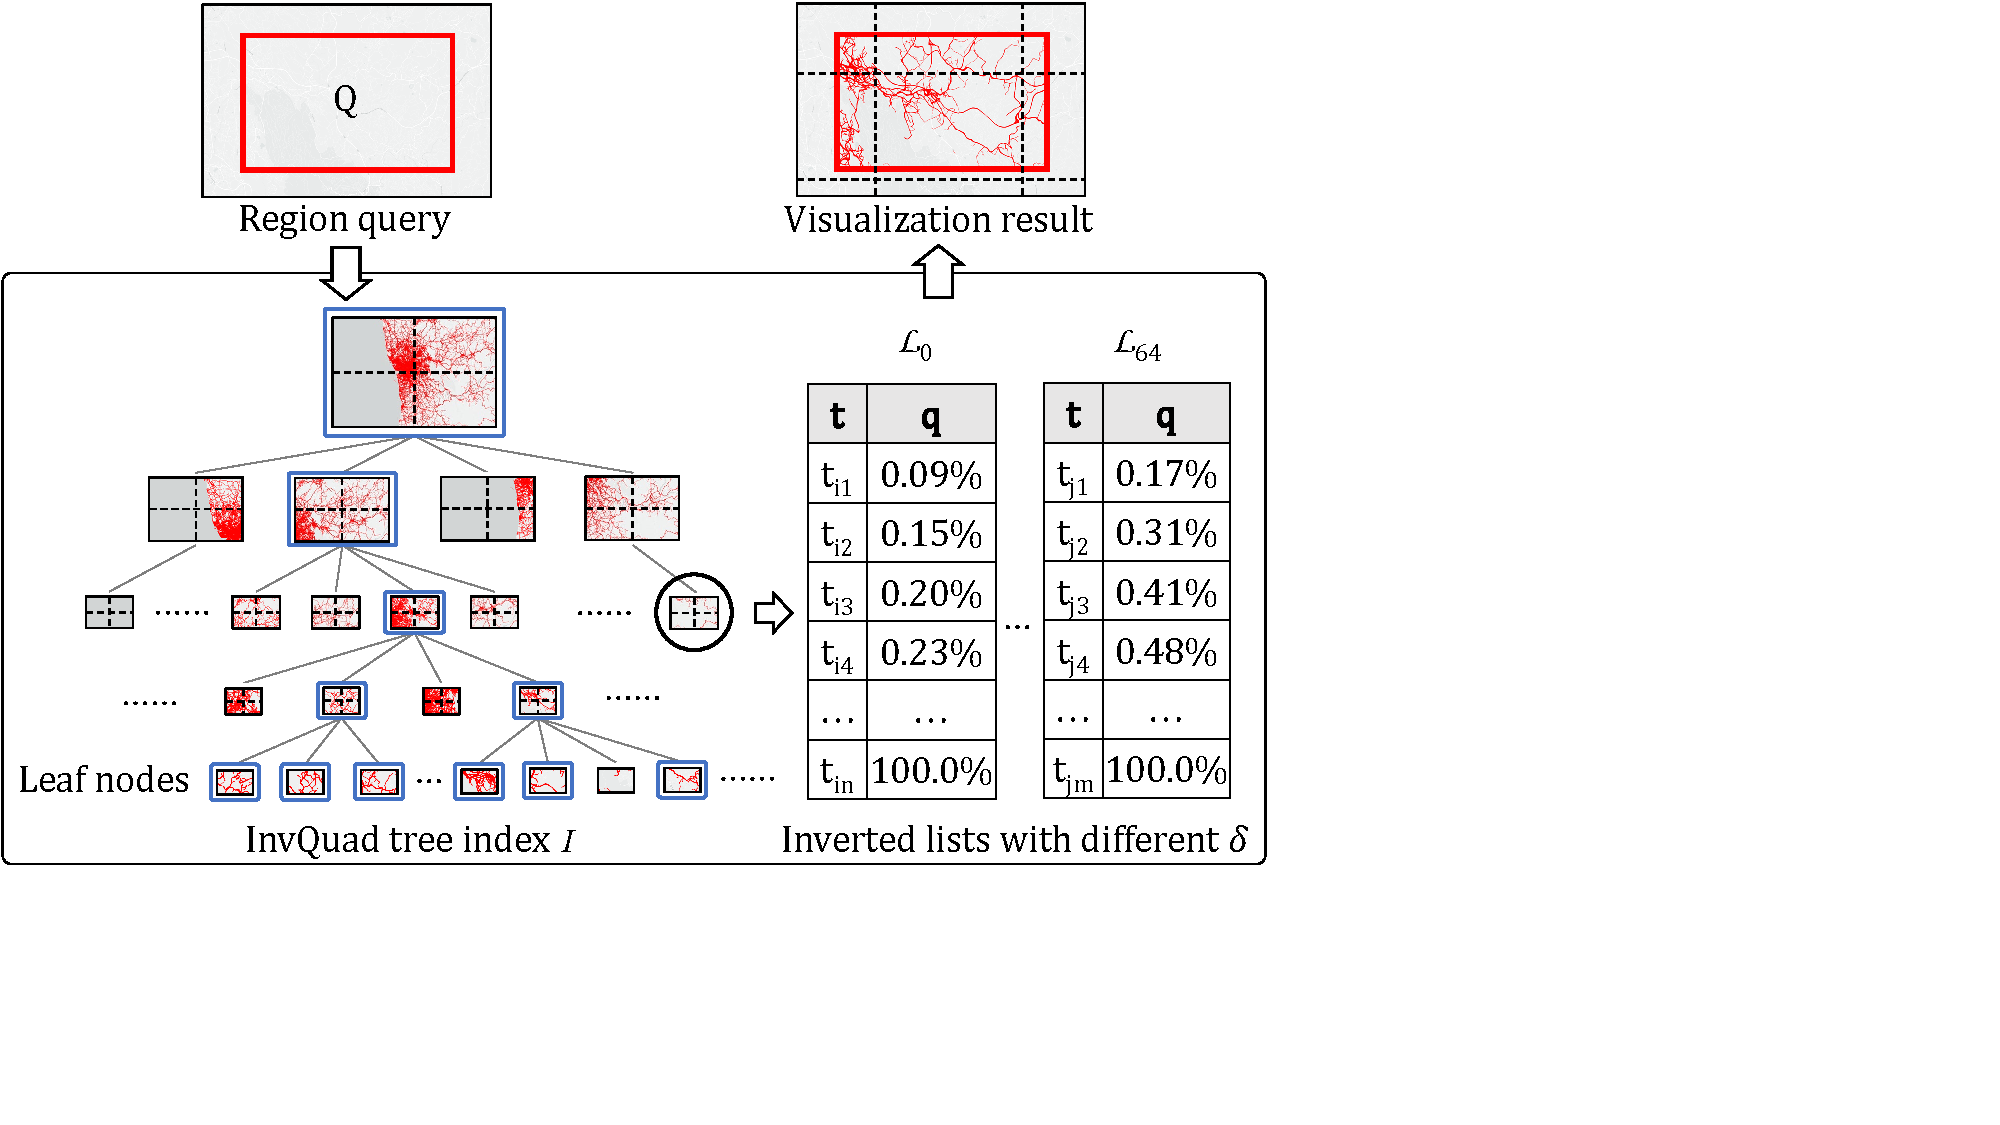
\includegraphics[width=0.47\textwidth]{pictures/cheetahtraj}
    \trim
    \caption{The $\avats$ framework}
    \label{fig:framework}
    \trim
\end{figure}


\subsection{Index Building}~\label{sec:index}
The key idea of $\avats$ is to conduct $\vatss$ sampling in the offline \emph{index building} phase such that the sampling results can be used directly for online visualization.
Specifically, we propose an inverted list augmented quad-tree index ($\invQ$) to handle arbitrary query region.

As shown in the example $\invQ$-tree index $\II$ at the bottom of Figure~\ref{fig:framework}, we exploit a quad-tree to recursively partition the entire area (spanned by the trajectory dataset) into smaller areas and manage each area with a tree node.
For each tree node, we run $\vatss$ using the trajectories (or trajectory segments) in its associated area as input to compute the \textit{visualization quality inverted lists} for this area. $\mathcal{L}_0$ and $\mathcal{L}_{64}$ in Figure~\ref{fig:framework} are two example visualization quality inverted lists, in which the subscripts are the values of $\delta$ for this list.
Specifically, we compute several inverted lists with different $\delta$ values\footnote{We set $\delta$ as 0 (i.e., $\vats$), 4, 8, 16, 32, 64. We need quality inverted lists with different $\delta$ for one area as the area may be covered by query regions of different sizes, and we use lists with larger $\delta$ for larger query region as discussed in Section~\ref{subsec:VQGS+}.} to support the efficient quality guaranteed result visualization at various zoom levels.
For each inverted list, (i) $\vatss$ terminates until the quality of the sample set is $100\%$, i.e., the visualization result of the sample set is the same as the full dataset;
(ii) the trajectory selected at each iteration of $\vatss$ is stored in the inverted list with its \textit{cumulative quality} in ascending order. Take inverted list $\mathcal{L}_0$ in Figure~\ref{fig:framework} for example, $t_{i4}$ is the trajectory selected at the $4$th iteration,
$t_{i4}$'s cumulative quality is $0.23\%$, which means that the quality achieved by $\{t_{i1}, t_{i2}, t_{i3}, t_{i4}\}$ as a whole is $0.23\%$. With the quality inverted list, searching a quality guaranteed sample set for a query region can be conducted efficiently via binary search.


\subsection{Query Processing}~\label{sec:query}
For a region visualization query $\query$ with quality threshold $\tau$, Algorithm~\ref{alg:query} summarizes the $\mathsf{Query}$ subroutine, which finds a quality guaranteed trajectory sample set $\oR$. The algorithm starts by invoking $\mathsf{Query}(\query, \tau, \II.root, \oR=\emptyset)$, i.e., from the root of $\invQ$-tree index $\II$ with an empty result set $\oR$. Then Algorithm~\ref{alg:query} transverses the tree nodes recursively. If node   $\mathcal{N}$ is a leaf node or its associated area is entirely contained in the query region, we retrieve a quality guaranteed trajectory set by calling subroutine $\mathsf{findRet}()$, which conducts binary search on the proper inverted list in $\mathcal{N}$ (Line~\ref{line:ret}). Otherwise, we call $\mathsf{Query}()$ on the four children nodes of $\mathcal{N}$ ( Line~\ref{line:valls}-\ref{line:valle}).


\begin{algorithm}
	\caption{$\mathsf{Query}$($\query$, $\tau$, $\invQ$ node $\mathcal{N}$, result $\oR$)}
	\label{alg:query}
	\begin{algorithmic}[1]
        \If{ $\mathcal{N}$ is leaf node or  $\mathcal{N}$ is entirely contained in $\query$}
            \State $\oR \leftarrow \oR \cup \mathsf{findRet}(\mathcal{N}, \tau)$ \label{line:ret}
        \ElsIf {$\query \cap \mathcal{N} \neq \emptyset$} \label{line:valls}
            \For { $i$ from $0$ to $3$}
                \State $\mathsf{tmpQ} \leftarrow \query \cap \mathcal{N}.child[i]$
                \State $\mathsf{Query}(\mathsf{tmpQ}, \tau, \mathcal{N}.child[i], \oR)$
            \EndFor \label{line:valle}
        \EndIf
	\end{algorithmic}
\end{algorithm}

Some trajectories in $\oR$, the result returned by $\mathsf{Query}()$ for region $\query$, may have segments outside $\mathcal{Q}$,
we conduct a way point query $\wpts(\query, \oR)$ to filter these segments before visualization.
%

\stitle{Correctness analysis}
We first show that $\avats$ meets the visualization quality requirement in Theorem~\ref{theorem:quality} as follows.

\begin{theorem}\label{theorem:quality}
If all selected nodes in the $\invQ$-tree index $\II$ are entirely contained in the query region $\query$,
then the result set $\oR$ returned by Algorithm~\ref{alg:query} satisfies that $\QQ(\oR) \ge \tau$.
\end{theorem}

\begin{proof}
Suppose query region $\query$ selects areas $\mathcal{A}_1,\!\mathcal{A}_2,\!\cdots,\!\mathcal{A}_K$,
these areas satisfy $\mathcal{A}_i \cap \mathcal{A}_j = \emptyset$ for $i\neq j$, and $\cup_{k=1}^{K}\mathcal{A}_k=\mathcal{Q}$.
For each area $\mathcal{A}_k$, denote the number of points marked in the ground truth visualization as $n_k$,
and the number of points marked by the trajectories in $\mathcal{R}$ as $m_k$,
we have $\frac{m_k}{n_k} \ge \tau$ as we use the visualization quality inverted index for trajectory selection.
Thus, for query region $\query$ with result set $\oR$, we have
$\QQ(\oR) = \frac{\sum_{k=1}^{K} m_k}{\sum_{k=1}^{K} n_k} \ge \tau.$
\end{proof}
In more general cases, we also select some areas that only intersect with the query region $\query$ and the sample set $\oR$ may not satisfy $\frac{m_k}{n_k}\ge \tau$ for these areas.
This does not significantly affect visualization quality for two reasons:
(i) these areas are the leaf nodes of the $\invQ$-tree index and thus reside on the border of the query region.
When exploring the map, human tends to move the region of interest to the screen center, where is more ``close'' to eyes~\cite{fitts_click}. %fitts,
%It is well known human eyes are much more sensitive to the center of a visualization than to the border, a.k.a., the fish eye effect~\cite{xxx};
(ii) the areas of the border regions are small w.r.t. the query region if the $\invQ$-tree has a sufficient height (i.e., the leaf nodes have a small area).

%In the worst case, we could include all the trajectories in the border regions into the result region $\oR$ to let them satisfy the quality requirement $\tau$.

%By searching the $\invQ$-tree index, $\vatss$ obtains a quality guaranteed sample trajectory set $\oR$ for any query region $\query$ without conducting on-line sampling. The \textit{result visualization} can process $\oR$ for short visualization latency.

%Note that we do not use the $\invQ$-tree index when the query region is too small (e.g., with zoom level larger than 17) because there are only a small number of trajectories and visualizing all of them does not take a long time.


%In summary, the $\vatss$ framework exploits the proposed $\invQ$-tree index and query processing subroutine $\mathsf{Query}$ to provide high quality trajectory visualization for any user region query with low latency.

%and (ii) The areas of the border regions are small w.r.t. the query region if the height of $\invQ$-tree index is large enough, which is shown in the following Lemma.

%\begin{lemma}\label{lemma:size}
%If the query region $\query$ is an $L\times L$ square and the leaf areas in the quad-tree has a size $l\times l$, then the border regions takes up at most $\frac{4(L-1)l}{L^2}$ of the overall area of the query region.
%\end{lemma}

%The result of Lemma~\ref{lemma:size} also generalize to rectangle query region and quad-tree areas. We omit its proof as it is straightforward. In the implementation, we use $\mathsf{Full}$ if the query region satisfies $L< 32*l$ because the query region is small and visualizing all trajectories in it does not take too much time. In this case, we ensure that the border regions that does not satisfy the quality requirement takes at most 12.1\% of the area of the query region.









%\begin{algorithm}
%	\caption{$\mathsf{CheetahTraj:Search}(\mathcal{Q}, q, \mathcal{P})$} \label{alg:local search}
%	\label{alg:local query}
%	\begin{algorithmic}[1]
%		\Require Query region $\mathcal{Q}$, quality target $q$, trajectory tree $\mathcal{P}$
%		\Ensure Set $\mathcal{R}$ of trajectories meeting quality target $q$ for $\mathcal{Q}$
%		\State $\mathcal{R}=\emptyset$, $\mathcal{I}=\emptyset$
%		\While{$(1)$}
%		\If{$\mathsf{Disjoint}(\mathcal{Q}, \mathcal{P}.\mathcal{A})==1$}
%		\State Break;
%		\EndIf
%		\If{$\mathsf{Contain}(\mathcal{Q}, \mathcal{P}.\mathcal{A})==1$}
%		\State $\mathcal{I}=\mathcal{I}\cup \mathcal{P}.\mathsf{Inv}(\mathcal{A})$; Break;
%		\EndIf
%		\If{$\mathsf{Interset}(\mathcal{Q}, \mathcal{P}.\mathcal{A})==1$}
%		\If{$\mathcal{P}$ has no childern}
%		\State $\mathcal{I}=\mathcal{I}\cup \mathcal{P}.\mathsf{Inv}(\mathcal{A})$; Break;
%		\Else
%		\State Search with $\mathcal{Q}$ and $q$ for all 4 children of $\mathcal{P}$
%		\EndIf	
%		\EndIf
%		\EndWhile
%		\For{each $\mathcal{P}.\mathsf{Inv}(\mathcal{A})$ in $\mathcal{I}$}
%		\State Find trajectory set $\mathcal{T}'$ for quality $q$ via binary search
%		\State $\mathcal{R}=\mathcal{R}\cup\mathcal{T}'$
%		\EndFor
%		\State $\mathcal{R}=\mathsf{WayPoint}(\mathcal{R}, \mathcal{Q})$
%		\State Return $\mathcal{R}$
%	\end{algorithmic}
%\end{algorithm}

%To motivate $\avats$, we analyze the visualization results and processing time of three solutions in Figure~\ref{fig:motivate} and Table~\ref{tab:motivate}, respectively.
%All three baselines use a \textit{way point query} to find the (segments of) trajectories in the query region as the first step.
%$\full$ visualizes all trajectories in the query region, $\rand$ randomly selects 1\% of the trajectories in the query region while $\vatss$ uses $\vatss$ (with $\delta=8$) to sample 1\% of the trajectories in the query region.
%In Table~\ref{tab:motivate}, we report the number of processed location points (i.e., via screen point mapping and rendering) in the bracket after visualization time.

%\begin{figure}%[t]
%	\centering
%	
\includegraphics[width=0.22\textwidth]{pictures/holder.jpg}
%	\caption{The visualization result of $\mathsf{Full}$, $\mathsf{Random}$ and $\vatss$}
%	\label{fig:motivate}
%\end{figure}
%
%\begin{table}
%	\centering
%	\small
%	\caption{Time decomposition for $\mathsf{Full}$, $\mathsf{Random}$ and $\vatss$ (ms)}
%	\label{tab:motivate}
%	\begin{tabular}{|c|c|c|c|c|} \hline
%			& \textbf{WayPoint}  &  \textbf{Sample} & \textbf{Visualization}  & \textbf{Total Time}\\ \hline
%		$\mathsf{Full}$ &  &  & &  \\ \hline
%		$\mathsf{Random}$ &  &  & &  \\ \hline
%		$\vatss$  &  & & &  \\ \hline
%	\end{tabular}	
%\end{table}



%\begin{algorithm}
%	\caption{$\mathsf{CheetahTraj:Index}(\mathcal{T}, \mathcal{A}, H)$}
%	\label{alg:local index}
%	\begin{algorithmic}[1]
%		\Require Set $\mathcal{T}$ of trajectories in area $\mathcal{A}$, tree height $H$
%		\Ensure Trajectory quad-tree $\mathcal{P}$ with visualization quality inverted index $\mathsf{Inv}(.)$ for each node in $\mathcal{P}$
%		\State Conduct $\vatss$ for the trajectories in $\mathcal{T}$
%		\For{each trajectory $t_i$ in $\mathcal{T}$}
%		\State Record tuple $(t_i, q_i)$, $q_i$ is the \textit{cumulative quality} of $t_i$
%		\EndFor
%		\State Create node $\mathcal{P}$ to store the $(t_i, q_i)$ tuples as $\mathsf{Inv}(\mathcal{A})$
%		\If{$H>0$ and $|\mathcal{T}|>m$}
%		\State Partition $\mathcal{A}$ evenly into 4 areas $\mathcal{A}_1$, $\mathcal{A}_2$, $\mathcal{A}_3$ and $\mathcal{A}_4$
%		\For{$i\in \{1,2,3,4\}$}
%		\State $\mathcal{T}_i=\mathsf{WayPoint}(\mathcal{T}, \mathcal{A}_i)$;
%		\State $\mathcal{P}_i=\mathsf{Index}(\mathcal{T}_i, A_i, H-1)$;
%		\EndFor
%		\State Use $\mathcal{P}_1$, $\mathcal{P}_2$, $\mathcal{P}_3$ and $\mathcal{P}_4$ as the children of $\mathcal{P}$
%		\EndIf
%		\State Return $\mathcal{P}$
%	\end{algorithmic}
%\end{algorithm}

%We can make the following observations from Figure~\ref{fig:motivate} and Table~\ref{tab:motivate}: (1) $\vatss$ provides visualization results very similar to $\mathsf{Full}$ and effectively reduces the visual clutter of $\mathsf{Full}$ in dense regions. In contrast, the visualization result of $\mathsf{Random}$ is significantly different from $\mathsf{Full}$. Although $\mathsf{Random}$ has a short total time, its poor quality renders it inapplicable. (2) $\mathsf{Full}$ has a long visualization time due to processing too many location points. $\vatss$ has short visualization time as it effectively reduces the number of processed locations by sampling. But it spends a long time to conduct sampling, which also results in a long total time. Therefore, the key insight of $\avats$ to conduct $\vatss$ sampling in  the offline index building phase such that the sampling results can be used directly for online visualization.



%The index building and query processing procedures of $\avats$ are described in Algorithm~\ref{alg:local index} and Algorithm~\ref{alg:local query}, respectively.
%For index building,  Algorithm~\ref{alg:local index} uses a quad-tree to recursively partition the entire area into smaller areas and manages each area with a tree node. For each area $\mathcal{A}$, Algorithm~\ref{alg:local index} builds a \textit{visualization quality inverted index} $\mathsf{Inv}(\mathcal{A})$ for the trajectories in it. Specifically, in each iteration of $\vatss$, we choose a trajectory $t_i$ and calculate the visualization quality $q_i$ achieved by all trajectories sampled so far. We arrange the $(t_i, q_i)$ tuples in increasing order of $q_i$ in $\mathsf{Inv}(\mathcal{A})$, i.e., store the trajectories sampled in earlier iterations of $\vatss$ at first in the array. Thus, searching the trajectories that meet a quality requirement $q$ for area $\mathcal{A}$ can be conducted via a binary search.




\section{Experimental Evaluation}\label{sec:exp}

In this part, we first present a case study of the visualizations provided by $\avats$ in Section~\ref{sec:case} to demonstrate its good visualization quality. In Section~\ref{sec:user}, we conduct a comprehensive user study to compare the visualization quality of different methods. In Section~\ref{sec:quality}, we quantitatively evaluate the visual quality and efficiency of $\avats$ and compare with the baselines.

\begin{table}
	\centering
	\small
	\caption{Statistics of the datasets used in the experiments}
	\begin{tabular}{|c|c|c|c|c|} \hline
		Dataset & No. of  & No. of GPS  & Maximum  \\
                & Trajectories & points & length \\ \hline
		\pt{}& 2,389,863 & 75,667,503 & 3,490 \\ \hline
		\sz{}& 3,066,861 & 53,527,890 & 2,268 \\ \hline
		\cd{}& 2,400,000 & 80,040,361 & 6,468 \\ \hline
	\end{tabular}	\label{tab:dataset}
\end{table}

%porto:总条数:2389863,总点数:75667503,最长:3490;  Shenzhen:总条数:3066861,总点数:53527890,最长:2268

\stitle{Experiment Settings} We conduct the experiments
using 3 real-world trajectory datasets: \pt{}, \sz{} and \cd{}.
\pt{}~\cite{pt} contains 2.39 million taxi trajectories and 75.67 million of GPS points, and the longest trajectory has 3,490 GPS points.
\sz{}~\cite{sz} consists of 3.07 million taxi trajectories with 53.53 million GPS points, and the longest trajectory has 2,268 GPS points.
\cd{}~\cite{cd} has 2.40 million taxi trajectories and 80.04 million GPS points, and the longest trajectory consists of 6,468 GPS points. 
The statistics of the datasets are summarized in Table~\ref{tab:dataset}. The experiments are conducted on a machine with an Intel i7-8700 CPU, 24 GB memory and an NVIDIA GeForce GTX1080 GPU with 8 GB on-chip memory, running on Windows 10. All methods are implemented using Java 1.8. UnfoldingMap 0.9.92~\cite{ufmaps} is used to provide interactive map and GPS mapping, and the Processing 3 library~\cite{p3} is used for rendering. All timing results are measured in single-thread mode. The datasets and source codes to reproduce our results are available at~\cite{code}.

\stitle{Competitors} We compare $\avats$ with three competitors, i.e., $\mathsf{Full}$, $\mathsf{Random}$ and $\mathsf{DTW}$. $\mathsf{Full}$ visualizes all trajectories in the user selected region while $\mathsf{Random}$ selects trajectories in the user selected region at random for visualization. $\mathsf{DTW}$ is based on the DTW distance between trajectories~\cite{borcan2012improving} and designed by us to select trajectories with good diversity. Specifically, $\mathsf{DTW}$ samples the trajectory that maximizes the aggregate DTW distance to all remaining trajectories in each step. We note that it takes $\mathsf{DTW}$ several days to run on the experiment datasets because it needs to compute expensive DTW distance (quadratic complexity w.r.t. trajectory length) between all trajectory pairs. For fair comparison, we ensure that $\mathsf{Random}$ and $\mathsf{DTW}$ use the same number of trajectories as $\avats$.




\subsection{Case Study}\label{sec:case}

We conduct case study on the \pt{} dataset to demonstrate the visualization quality of $\avats$. Similar phenomenons are also observed on the other datasets and we omit their results for conciseness.

\begin{figure*}[t]
	\centering
	\includegraphics[width=1\textwidth]{pictures/case_study_icde/case_study_detail.pdf}
	\trim
	\caption{Case study of the visualization quality of $\avats$ for two detail regions.}
	\label{fig:detailview}
	\trim \trim
\end{figure*}

\subsubsection{Overview visualization}

We illustrate the visualization results of different methods for the entire \pt{} dataset in Figure~\ref{fig:overview}.

\stitle{Good visual quality for overview}
At zoom level 11, Figure~\ref{fig:overview}(A) is the visualization result of $\mathsf{Full}$ on the \pt{} dataset.
With a sampling rate $\alpha \!=\! 1\%$, Figures~\ref{fig:overview}(B), (C) and (E) are the visualizations produced by $\mathsf{Random}$, $\mathsf{DTW}$,
and $\avats$, respectively. Comparing with Figure~\ref{fig:overview}(B) and (C), it is obvious that Figure~\ref{fig:overview}(E) is more similar to Figure~\ref{fig:overview}(A). In particular, Figure~\ref{fig:overview}(E) not only preserves the overall visual structure of the entire region but also keeps the details of cities that are far from the center (marked by the dashed cycles in the figure). However, the details of these cities are lost in Figure~\ref{fig:overview}(B) as $\mathsf{Random}$ is more likely to select trajectories in the dense region. $\mathsf{DTW}$ in Figure~\ref{fig:overview}(C) preserves more details than $\mathsf{Random}$ in the sparse regions as it considers diversity in trajectories but its visualization quality is still inferior compared with $\avats$ in Figure~\ref{fig:overview}(E).

\stitle{Good visual quality under different sampling rates}
Figure~\ref{fig:overview}(D) and (E) are the visualizations produced by $\avats{}$ with a sampling rate of $0.1\%$ and $1\%$, respectively. We can make two observations: (i) the larger the sampling rate, the better the visual quality, i.e., Figures~\ref{fig:overview}(E) is more similar to Figure~\ref{fig:overview}(A) compared with Figure~\ref{fig:overview} (D); (ii) the visualization of $\avats$ with a sampling rate of $0.1\%$ (i.e., Figure~\ref{fig:overview}(D)) looks more appealing than the visualizations of $\mathsf{Random}$ and $\mathsf{DTW}$ with a sampling rate of $1\%$ (i.e., Figure~\ref{fig:overview}(B) and (C)) as Figure~\ref{fig:overview}(D) better preserves the visual structures of Figure~\ref{fig:overview}(A).



\stitle{Color encoding effectively mitigates visual clutter} At zoom level 11 and with a sampling rate of $1\%$, Figures~\ref{fig:overview}(E) and (F) are the visualizations produced our $\avats$ and $\cavats$ (i.e., $\avats$ with color encoding), respectively.
Visual clutter is severe for $\mathsf{Full}$ (i.e., Figure~\ref{fig:overview}(A)) and $\avats$ (i.e., Figure~\ref{fig:overview}(E)) because many pixels are visualized for the dense region in the center, which makes it difficult to identify the main routes. The visualization of $\cavats$ in Figure~\ref{fig:overview}(F) alleviates this problem by encoding more representative trajectories with warmer color, making it easier to identify some prominent routes than Figure~\ref{fig:overview}(A) and (E).

\vspace{1mm}
\subsubsection{Detail visualization}\label{sec:detail}




We analyze the visualizations produced by different methods for small areas with details by investigating two regions of interest in the \pt{} dataset in Figure~\ref{fig:detailview}.

%We next present the effectiveness of our proposals with detail views by investigating two regions of interest in \pt{}, the dense region B and the sparse region C(shown as in Figure~\ref{fig:detailview}(8)).

%$\mathsf{Full}$
%$\mathsf{DTW}$
%$\mathsf{Random}$



\stitle{Reduce visual clutter and preserve micro structures for dense region} At zoom level 15, region B in Figure~\ref{fig:detailview}(A) is the center of Porto and has the highest concentration of trajectories. Therefore, $\mathsf{Full}$ suffers from severe visual clutter and it is difficult to identify the road networks in Figure~\ref{fig:detailview}(B1).  $\mathsf{Random}$ and $\mathsf{DTW}$ in Figure~\ref{fig:detailview}(B2) and (B3) reduce the visual clutter to some extent by sampling some trajectories. $\avats$ in Figure~\ref{fig:detailview}(B4) is more successful in reducing the visual clutter of $\mathsf{Full}$ and allows to identify a much larger number of routes. In addition, $\avats$ preserves more micro structures of the trajectories than $\mathsf{Random}$ and $\mathsf{DTW}$, e.g., the circular route in the dashed circular region.

% and causes serious visual clutter, as visualized in Figure~\ref{fig:detailview}(B1).
%For example, the circular structures of the main route(shown as the dashed circular region in Figure~\ref{fig:detailview}(B1)) is unclear.
%$\localavats$ alleviates the visual clutter by preserve the $1\%$ trajectories of the total regions but the clutter is still serious. Furthermore, $\avats$ performs better than $\localavats$ by preserving less trajectories and reduce the visual clutter.


\stitle{Preserve overall layout for sparse region}
At zoom level 14, region C in Figure~\ref{fig:detailview}(A) contains the city of Casino Espinho and has fewer trajectories than the dense region in the center. In this case, the sampling methods need to keep the overall layout of the trajectories  to provide good visualization quality. Compared with $\mathsf{Full}$ in Figure~\ref{fig:detailview}(C1), $\mathsf{Random}$ and $\mathsf{DTW}$ in Figure~\ref{fig:detailview}(C2) and (C3) fail to meet this requirement as they do not show any trajectory for areas far from the city, e.g., in the dashed circle. This makes their entire visualization layout very different from $\mathsf{Full}$. In contrast, $\avats$ in Figure~\ref{fig:detailview}(C4) preserves the trajectories in areas far from the city and has a overall layout similar to $\mathsf{Full}$.

%Region C includes the city of Casino Espinho at zoom level 14, which contains less trajectories than the center of Porto as the visualization result of full dataset shown in Figure~\ref{fig:detailview}(C1).
%Given fix sampling rate $\alpha=1\%$, Figure~\ref{fig:detailview}(C2) indicates the visualization of $\localavats$. This visualization result misses a lot if detail information in this region, because the fix sampling rate preserves too few trajectories which is difficult to guarantee the visual quality.
%While $\avats$ in Figure~\ref{fig:detailview}(C3) performs much better than $\localavats$ as the sampling rate is automatically adjusted to according to the visual quality. In this visualization, the trajectory sketch of Casino Espinho is almost the same as it in Figure~\ref{fig:detailview}(C1), the visualized result of full dataset.

To sum up, the case study shows that $\avats$ effectively mitigates visual clutter with sampling and color encoding. With the quality-aware $\vatss$ sampling algorithm, $\avats$ also provides better visualization quality than $\mathsf{Random}$ and $\mathsf{DTW}$ by preserving the micro structures and overall layout of full visualization.

\subsection{User Study}\label{sec:user}

\begin{figure*}
     \centering
     \begin{tabular}{ccc}
		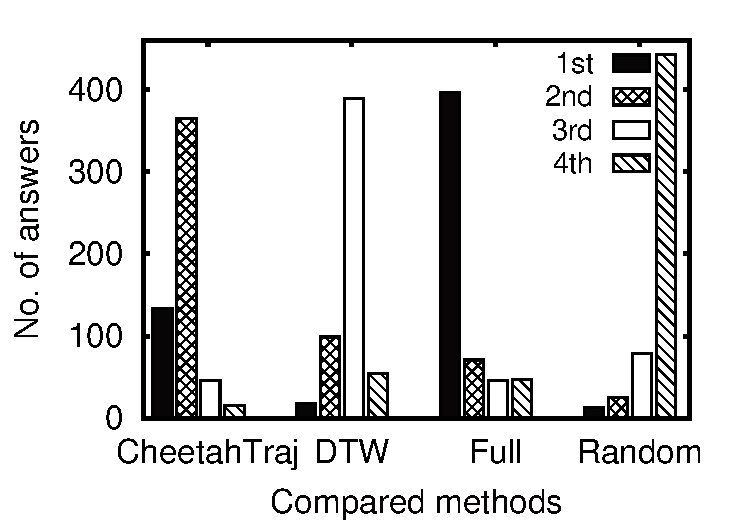
\includegraphics[width=0.6\columnwidth]{pictures/user_study/quality}
		&
		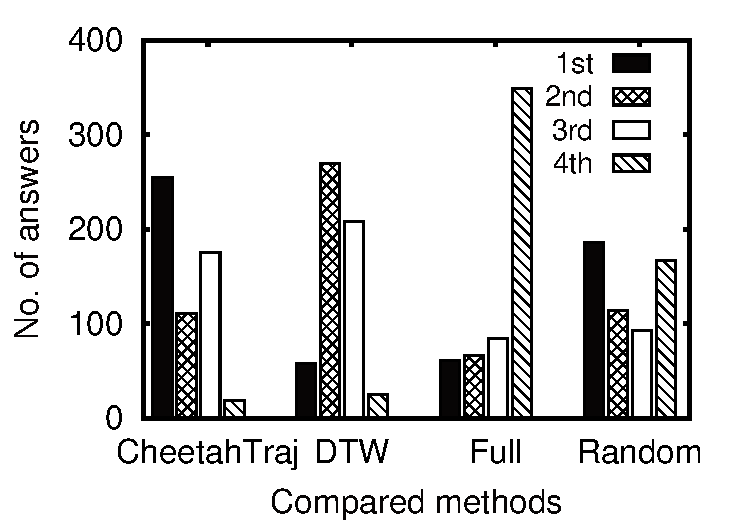
\includegraphics[width=0.6\columnwidth]{pictures/user_study/clutter}
        &
        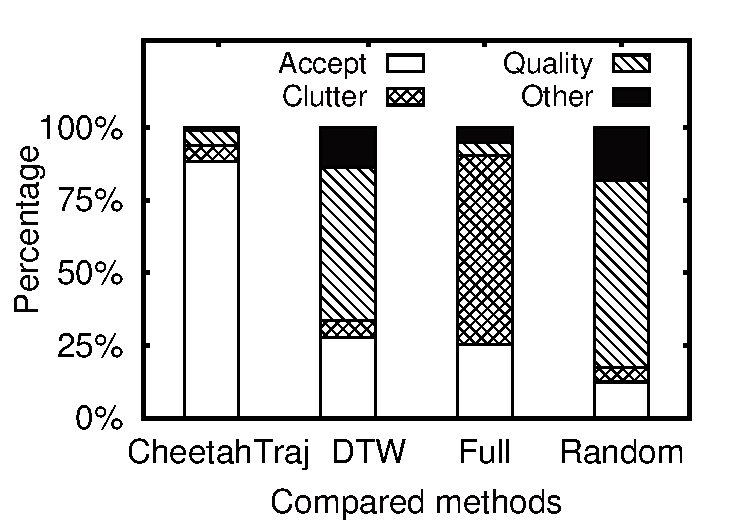
\includegraphics[width=0.6\columnwidth]{pictures/user_study/accept}
		\\
		(A) T1: visual quality study
		&
		(B) T2: visual clutter study
        &
        (C) T3: acceptable visualization study
	\end{tabular}
	\caption{User study results of different visualization methods}
	\label{fig:userstudy}
    \trim
\end{figure*}

In this part, we conduct a user study to evaluate the quality of visualizations generated by different methods objectively.

\stitle{Settings}
We recruited 35 participants with 10 females, 25 males, aged 19 to 31 with a mean of 24.78 for the user study. 
The user study is conducted on the \pt{} and \sz{} datasets, and four visualization methods are investigated, i.e., $\full$, $\rand$, $\mathsf{DTW}$ and $\avats$. We manually select 22 \textit{center points} in the two datasets and define 3 \textit{visualization scales} including:
large-scale region (with zoom level smaller than 13), middle-scale region (with zoom level between 13 and 15), small-scale region (with zoom level larger than 15). For each center point and at each visualization scale, we generate a \textit{comparable visualization group}, which includes one visualization generated by each of the 4 methods. This results in 66 comparable groups (22 center points $\times$ 3 scales) and 264 visualization results (66 comparable groups $\times$ 4 visualizations).

We are interested in the visual quality and visual clutter of the visualizations, and hence designed three tasks for a comparable group:
\begin{itemize}
	\item Task 1 (T1): rank the visualizations in a group from the highest visual quality to the lowest visual quality by 1st, 2nd, 3rd, and 4th.
	\item Task 2 (T2): rank the visualizations in a group from the least visual clutter to the most severe visual clutter by 1st, 2nd, 3rd, and 4th.
	\item Task 3 (T3): select the visualizations considered acceptable (multiple choices allowed) and choose the reason for the visualizations considered unacceptable. We provide three reasons including ``severe visual clutter", ``poor visual quality" and ``others".
\end{itemize}

The user study system is a web-based platform, in which all visualizations are displayed with a resolution of 450*300.


\stitle{User study procedure} When the participants enter the user study system, they are given a tutorial on how to conduct the tasks to get familiar with the interface and tasks.
For each participant, we randomly select 16 comparable groups.
Thus, we obtain $35 \times 16 = 560$ results for each task.
For each comparable group, the 4 visualizations (\textit{without specifying generated by which method}) in it are displayed on the same web-page and a participant is required to perform task T1, T2 and T3 by inspecting them.

%At last, the participants are interviewed to collect feedback after finishing the study and their answers are saved for result analysis.



\stitle{Result analysis} Figure~\ref{fig:userstudy}(A) reports the visual quality ranking of the 4 methods in T1. 
The results show that $\full$ ranks the 1st in most cases while $\avats$ usually ranks 1st or 2nd, i.e., the percentage of $\avats$ ranks top-2 among 4 methods is $88.9\%$. 
In contrast, $\mathsf{DTW}$ and $\rand$ rank 3rd and 4th at most times. 
This suggests that the visualizations generated by $\avats$ are more appealing to the participants than $\mathsf{DTW}$ and $\rand$. 
We also observed that the participants tend to rank $\avats$ before $\full$ for large-scale regions with  many trajectories, and the other way for smaller regions. 


Figure~\ref{fig:userstudy}(B) reports the anti-visual clutter ranking of the 4 methods in T2. 
The results show that visual clutter is most severe for $\full$, ranking 4th in most cases (349 over 560). With sampling, $\mathsf{DTW}$ usually rank 2nd and 3rd but $\rand$ ranks 4th for a considerable number of times as it tends to create clutter in the dense regions.    
$\avats$ is the most successful in reducing visual clutter, ranking 1st in 255 out of the 560 cases and ranking 4th for only 19 cases.    



We report the frequency each of the 4 methods is selected as acceptable and why a method is not selected in T3 using bar chart in Figure~\ref{fig:userstudy}(C). 
Each column corresponds to a method, and from bottom to top, the lengths of the bars indicate the percentage of participants choosing ``acceptable'', ``not acceptable due to visual clutter'', ``not acceptable due to poor visual quality'' and ``not acceptable for other reasons''. 
The results show that $\avats$ is regarded acceptable for about 88.2\% of the cases, and the other methods have significantly lower acceptance rate than $\avats$. 
Specifically, $\mathsf{DTW}$ and $\rand$ have low acceptance rate mainly due to poor visual quality while $\full$ suffers from severe visual clutter.


%Figure~\ref{fig:rank} left shows the ranking among different methods with x-axis indicating the ranking from the highest quality to the lowest quality and y-axis indicating the selecting number for the specific method and ranking. The visualization of $\full$ has the highest visual quality since it has no information loss according the quality definition. The selection of $\avats$ is mostly concentrated at the first and second, which is closely behind the $\full$. The selections of $\baseline$ and $\rand$ are contracted at the third and fourth respectively, which is confirmed both of these two methods performs worse than $\full$ and $\qtavats$ in guarantee the visual quality.



%Figure~\ref{fig:rank} right reports the ranking among different methods with x-axis indicating the ranking from the least clutter to the most clutter and y-axis indicating the total selecting number for the specific method and ranking. We observe that the $\qtavats$ is ranked at the first 155 times which is significantly more than the other methods. The number it ranks at the second, third and last are 68, 96 and 14. There is no doubt that the visualization of $full$ suffers the most sever visual clutter problem because 210 of 333 total answers rank $full$ at the fourth, while other methods can be used to help to reduce the visual clutter.



%\begin{figure}[t]
%	\centering
%	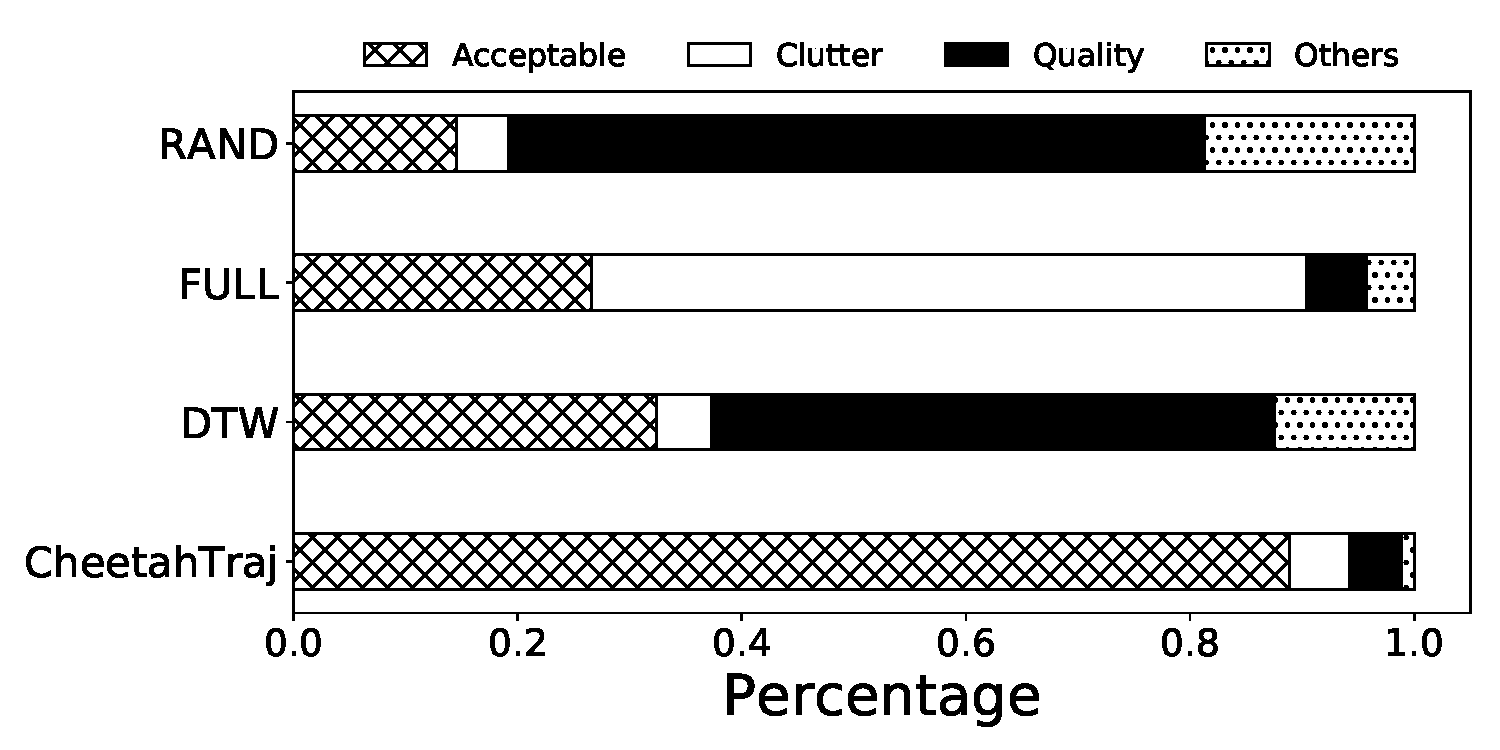
\includegraphics[width=0.35\textwidth]{pictures/user_study/accept_rate.pdf}
%	%\vspace{-5mm}
%	\caption{User study, accept rate.}
%	\label{fig:accept_rate}
%	%\vspace{-8mm}
%\end{figure}






\begin{figure*}
	\centering
	\small
	\begin{tabular}{ccc}
		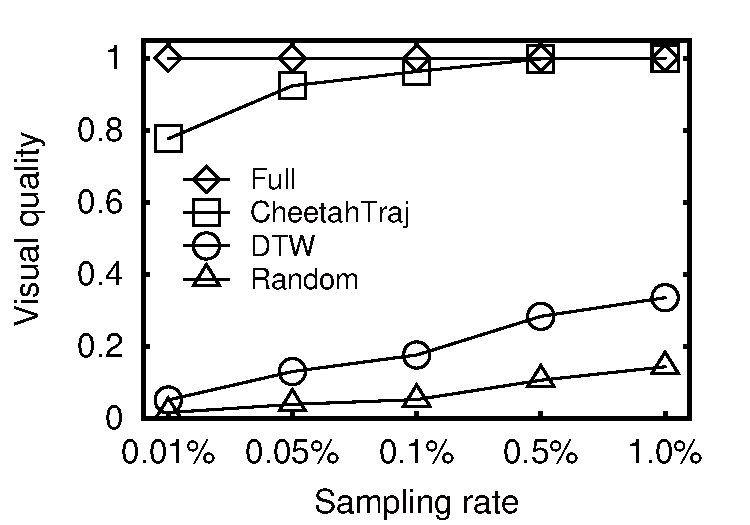
\includegraphics[width=0.3\linewidth]{pictures/quantitative_study/rate_porto_q}
		&
		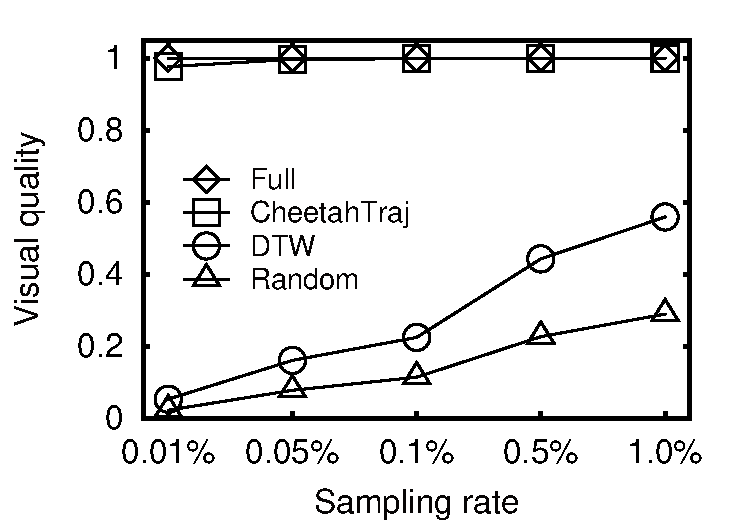
\includegraphics[width=0.3\linewidth]{pictures/quantitative_study/rate_sz_q}
        &
		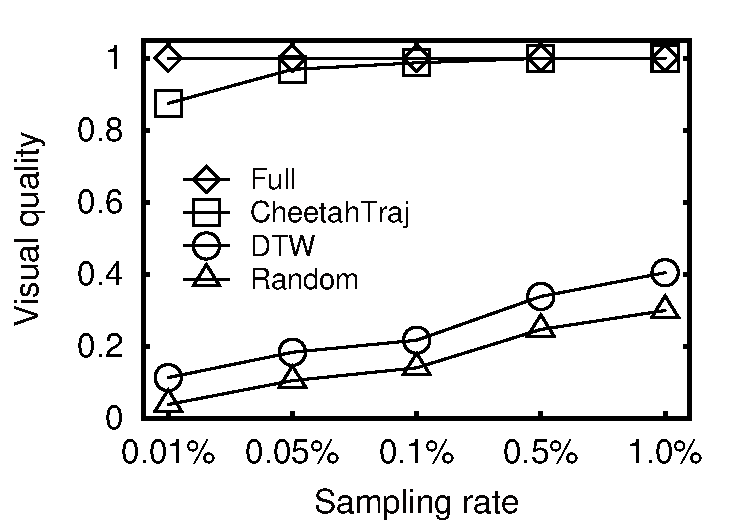
\includegraphics[width=0.3\linewidth]{pictures/quantitative_study/rate_cd_q}
		\\
		(A) \pt{}
		&
		(B) \sz{}
		&
		(C) \cd{}
	\end{tabular}
    \trim
	\caption{Effect of varying sampling rate visual quality.}
	\label{fig:rate_quality}
	\trim \trim
\end{figure*}

\begin{figure*}
	\centering
	\small
	\begin{tabular}{ccc}
		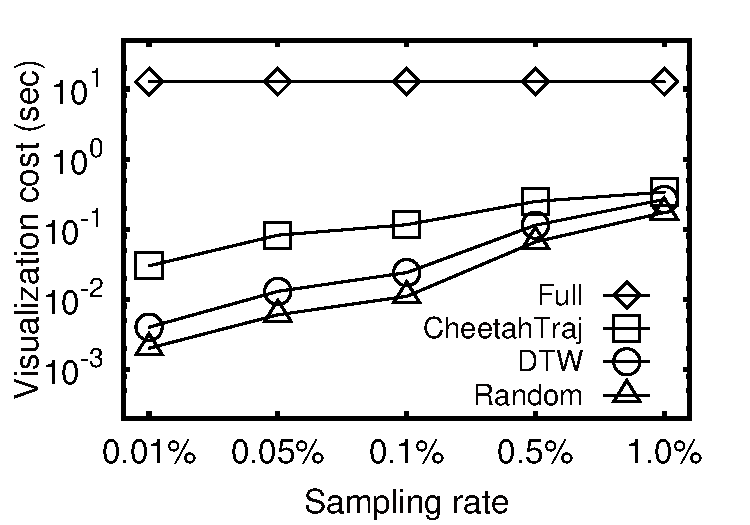
\includegraphics[width=0.3\linewidth]{pictures/quantitative_study/rate_porto_t}
		&
		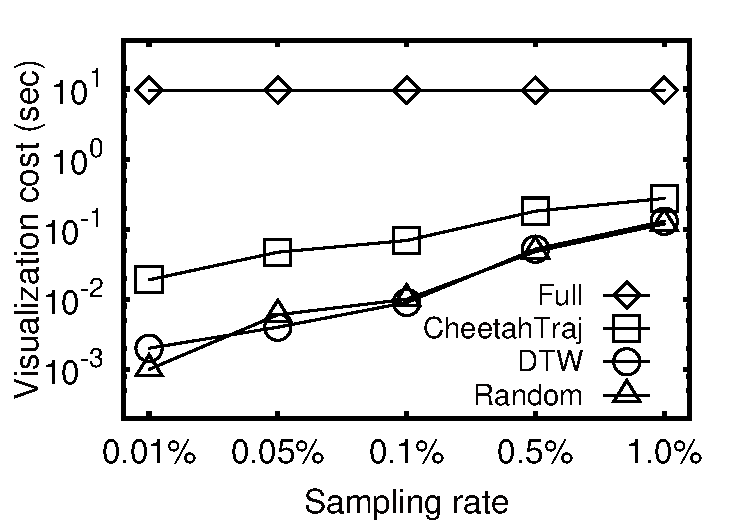
\includegraphics[width=0.3\linewidth]{pictures/quantitative_study/rate_sz_t}
        &
		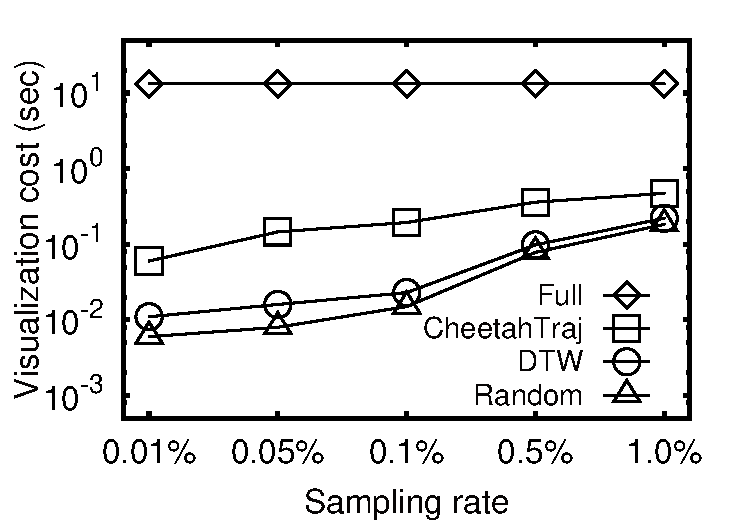
\includegraphics[width=0.3\linewidth]{pictures/quantitative_study/rate_cd_t}
		\\
		(A) \pt{}
		&
		(B) \sz{}
		&
		(C) \cd{}
	\end{tabular}
    \trim
	\caption{Effect of  sampling rate on visualization cost.}
	\label{fig:rate_vistime}
	\trim \trim
\end{figure*}

\begin{figure*}
	\centering
	\small
	\begin{tabular}{ccc}
		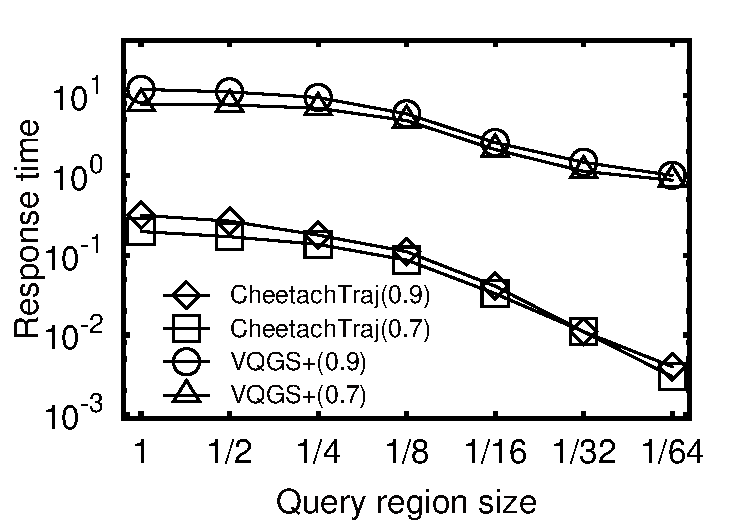
\includegraphics[width=0.3\linewidth]{pictures/quantitative_study/size_porto_t}
		&
		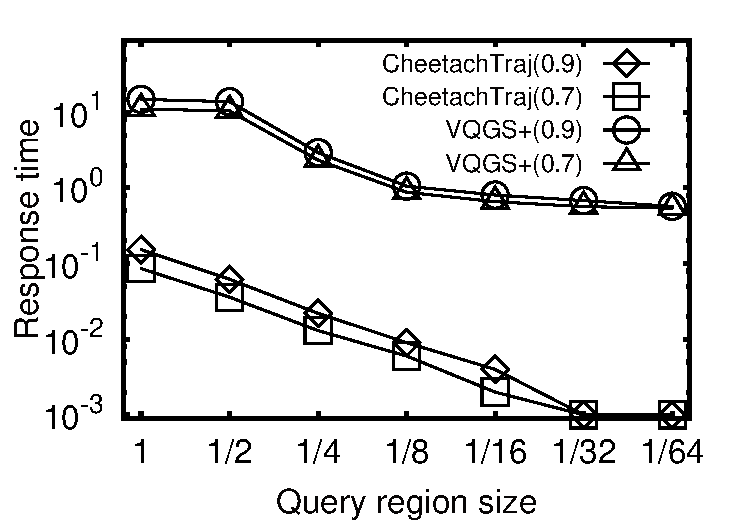
\includegraphics[width=0.3\linewidth]{pictures/quantitative_study/size_sz_t}
		&
		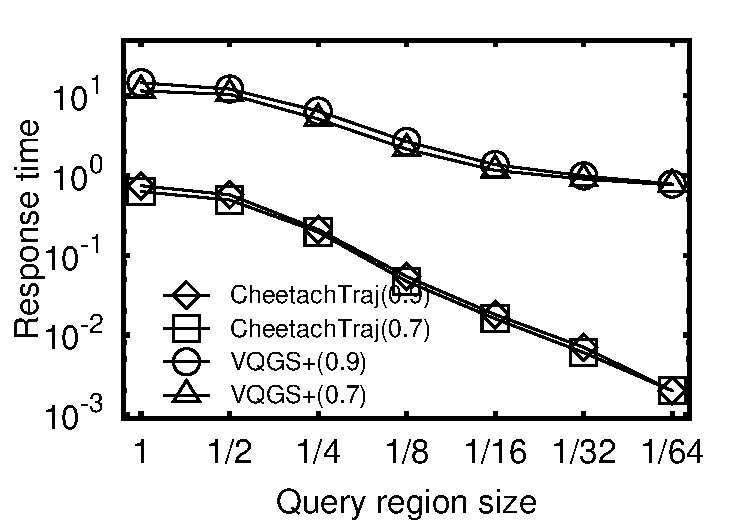
\includegraphics[width=0.3\linewidth]{pictures/quantitative_study/size_cd_t}
		\\
		(A) \pt{}
		&
		(B) \sz{}
		&
		(C) \cd{}
	\end{tabular}
    \trim
	\caption{Effect of region size on end-top-end response time.}
	\label{fig:size_responsetime}
	\trim \trim
\end{figure*}


\begin{figure*}
	\centering
	\small
	\begin{tabular}{ccc}
		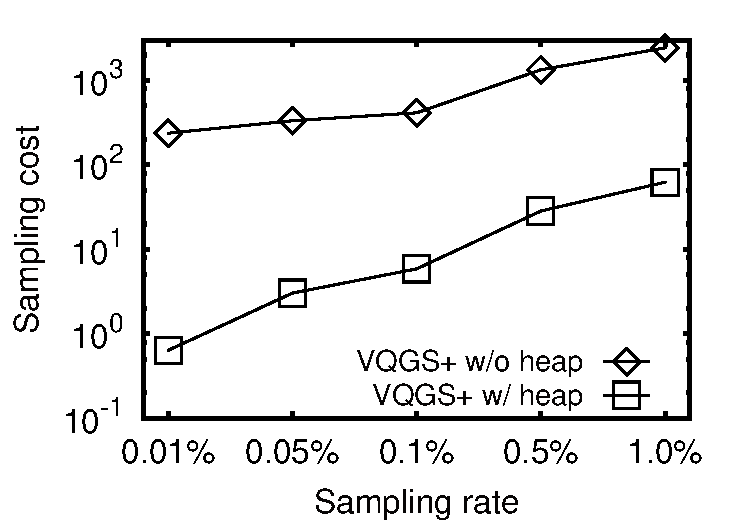
\includegraphics[width=0.3\linewidth]{pictures/quantitative_study/vqgs_porto_t}
		&
		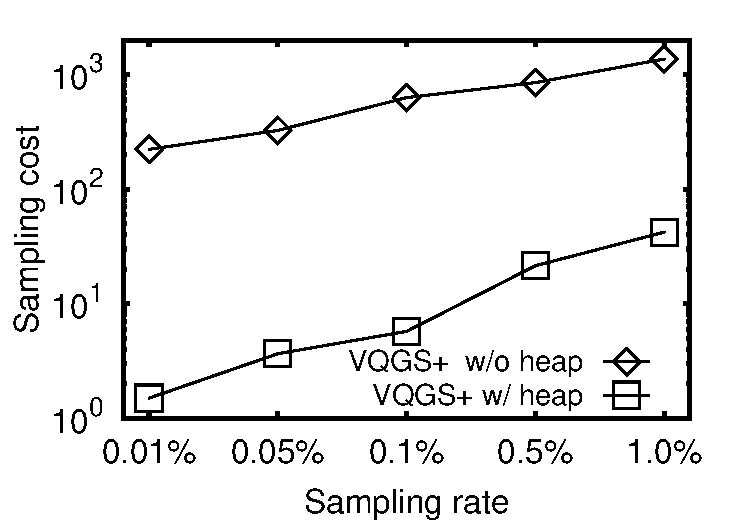
\includegraphics[width=0.3\linewidth]{pictures/quantitative_study/vqgs_sz_t}
		&
		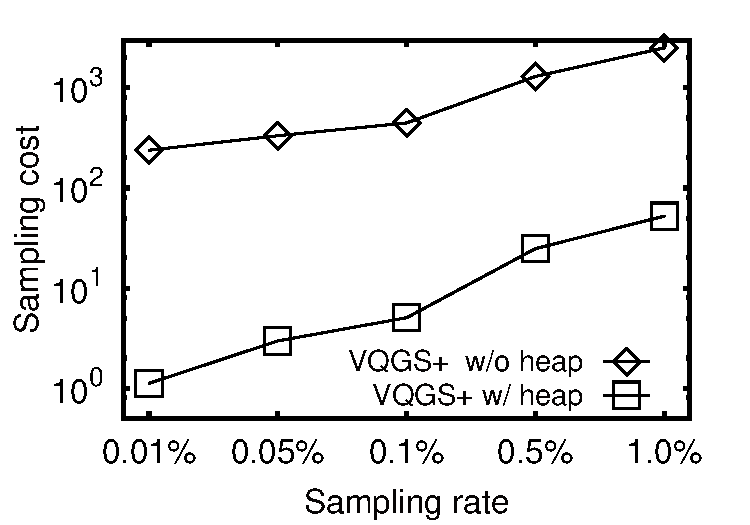
\includegraphics[width=0.3\linewidth]{pictures/quantitative_study/vqgs_cd_t}
		\\
		(A) \pt{}
		&
		(B) \sz{}
		&
		(C) \cd{}
	\end{tabular}
    \trim
	\caption{Effect of sampling rate on the sampling cost of $\vatss$ with/without optimization}
	\label{fig:rate_algtime}
	\trim \trim
\end{figure*}

\subsection{Quantitative Evaluation}\label{sec:quality}
In this part, we quantitatively evaluate the visual quality and efficiency of $\avats$ on the three real-world trajectory datasets.

\stitle{Visual quality} Figure~\ref{fig:rate_quality} reports the visualization quality (as defined in Equation~\eqref{eqref:loss}) of the methods under different sampling rate.
We consider the entire region in each dataset for this experiment.
The results show that our proposal $\avats$ achieves significantly higher quality than $\rand$ and $\mathsf{DTW}$ under the same sampling rate.
This is because the sampling algorithm $\vats$ and $\vatss$ in the $\avats$ framework are designed with explicit considerations for visual quality.
Specifically, the quality of $\avats$ approaches 1 when the sampling rate is still less than 1\% for all 3 datasets.
$\mathsf{DTW}$ has a higher quality than $\rand$ because it considers the diversity of trajectories.


In Figure~\ref{fig:rate_vistime}, we report the visualization cost (i.e., the wall clock time to generate visualization result using the sampled trajectories) for the methods under different sampling rate.
We still consider the entire region in this experiment and the visualization time of $\full$ (which does not change with sampling rate) is included at the top of each figure for reference.
The results show that all sampling methods achieve significantly shorter visualization cost than $\full$, and the speedup can be 1 to 4 orders of magnitude.
This confirms our observation that sampling is effective in improving visualization efficiency.
Under the same sampling rate, our $\avats$ takes slightly longer visualization time than $\rand$ and $\mathsf{DTW}$
because $\avats$ tends to select long trajectories for quality maximization.
%It is worth to point out the largest visualization cost of $\avats$ in \pt{}, \sz{} and \cd{} are 0.339, 0.275 and 0.471
Combining Figure~\ref{fig:rate_quality} and~\ref{fig:rate_vistime}, we can conclude that $\avats$ can achieve high visualization quality with  short visualization latency.


\stitle{Efficiency of $\avats$}
We evaluate the \textit{response time} of our $\avats$ framework under different quality guarantees and region sizes in Figure~\ref{fig:size_responsetime}.
The response time of $\avats$ is the end-to-end time for generating visualization for a selected region, which includes querying the $\avats$ index and computing the visualization.
For comparison, we also plot the response time of $\vatss$ (with $\delta\!=\!8$), which uses on-line sampling instead of querying the index in $\avats$ framework.
We constrain the regions to be rectangles with a constant height/width ratio and measure the size of a region by dividing its height over the height of the entire region.
For each region size, we report the average response time of three typical regions, i.e., a dense region, a sparse region and a medium region.
The results show that $\avats$ achieves a short response time (less than 1 second in all cases and 0.2 second for most cases) for different region sizes and quality guarantees. $\vatss$ is 1 to 2 orders of magnitude slower than $\avats$ and takes at most 14.802 seconds in all cases. These results show that $\vatss$ cannot support interactive visual exploration and the $\invQ$-tree index in $\avats$ is effective in improving efficiency.
In addition, the response time decreases rapidly when the region size shrinks as there are fewer trajectories in a smaller region.
However, the response time required to achieve a high quality (e.g., 0.9) is not significantly longer than a low quality (e.g., 0.7) as quality improves quickly with the number of sampled trajectories as a shown in Figure~\ref{fig:rate_quality}.





\stitle{Effect of heap-based lazy computation}
In Figure~\ref{fig:rate_algtime}, we report the running time of $\vatss$  with and without the heap-based lazy computation.
The results show that the heap-based optimization reduces the running time of $\vatss$ around 2 orders of magnitude.
For the sampling rates we considered, $\vatss$ runs efficiently and can finish within 1 second for the entire dataset.



%\begin{figure}[t]
%	\centering
%	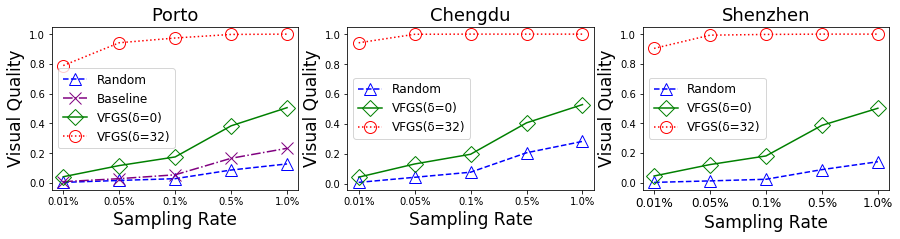
\includegraphics[width=0.5\textwidth]{pictures/quantitative_study_icde/sample_quality.png}
%	\vspace{-8mm}
%	\caption{Visual quality vs. sampling rates.}
%	\label{fig:sample_quality}
%	\vspace{-3mm}
%\end{figure}

%\begin{figure}[t]
%	\centering
%	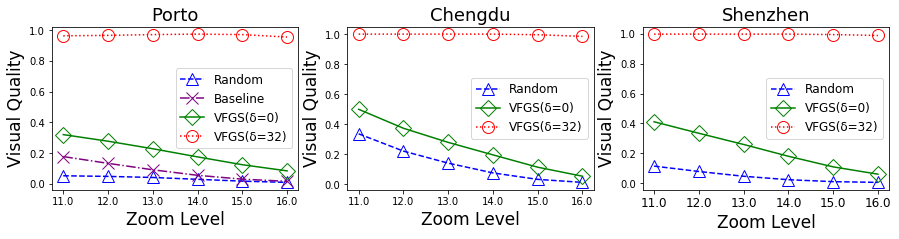
\includegraphics[width=0.5\textwidth]{pictures/quantitative_study_icde/zoom_quality.png}
%	\vspace{-8mm}
%	\caption{Visual quality vs. zoom level.}
%	\label{fig:zoom_quality}
%	\vspace{-3mm}
%\end{figure}


%\begin{table}
%	\centering
%	\small
%	\caption{The cost of $\invQ$-tree index}
%	\begin{tabular}{|@{}c@{}|@{}c@{}|@{}c@{}|@{}c@{}|@{}c@{}|} \hline
%		Dataset (size) & Height & Building time & Memory size \\ \hline
%		\pt{} (1.44G)	& 13 & 526.390s & 3.65GB  \\ \hline
%		\sz{} (1.02G)	& 13 & 435.291s  & 3.12GB \\ \hline
%		\cd{} (1.49G)	& 13 & 454.151s & 3.71GB \\ \hline
%	\end{tabular}	\label{tab:index cost}
%    \trim %\trim
%\end{table}

\begin{table}
	\centering
	\small
	\caption{The cost of $\invQ$-tree index}
	\begin{tabular}{|c|c|c|c|} \hline
		Dataset (size) & Height & Building time & Memory size \\ \hline
		\pt{} (1.44G)	& 13 & 526.390s & 3.65GB  \\ \hline
		\sz{} (1.02G)	& 13 & 435.291s  & 3.12GB \\ \hline
		\cd{} (1.49G)	& 13 & 454.151s & 3.71GB \\ \hline
	\end{tabular}	\label{tab:index cost}
	\trim %\trim
\end{table}

\stitle{$\invQ$-tree index cost evaluation}
We report the building time and memory cost of the $\invQ$-tree index in Table~\ref{tab:index cost}.
For all three datasets, it takes less than 10 minutes to build the $\invQ$ index with a height of 13.
The memory cost of the $\invQ$ index in the last column is also comparable with the size of the raw data shown in the first column.




%\stitle{Running time evaluation}

%\begin{figure}[t]
%	\centering
%	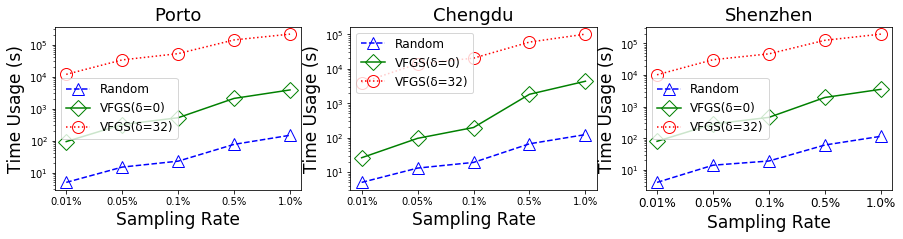
\includegraphics[width=0.5\textwidth]{pictures/quantitative_study_icde/sample_time.png}
%	\vspace{-8mm}
%	\caption{Time usage vs. sampling rates.}
%	\label{fig:sample_time}
%	\vspace{-3mm}
%\end{figure}

%\begin{figure}
%	\centering
%	\small
%	\begin{tabular}{cc}
%		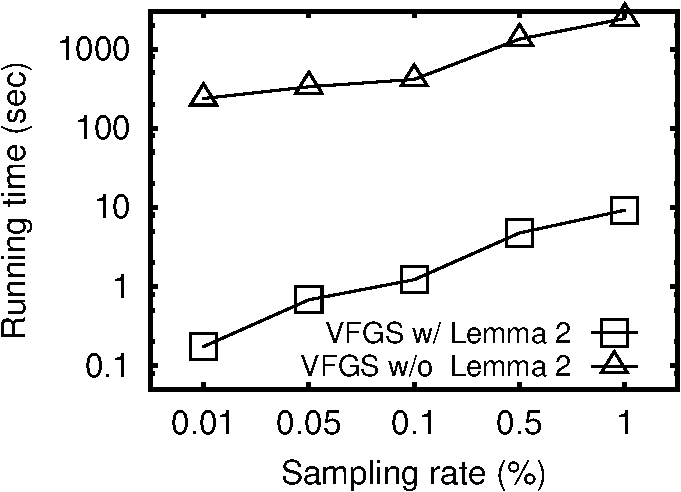
\includegraphics[width=0.44\columnwidth]{pictures/tporto}
%		&
%		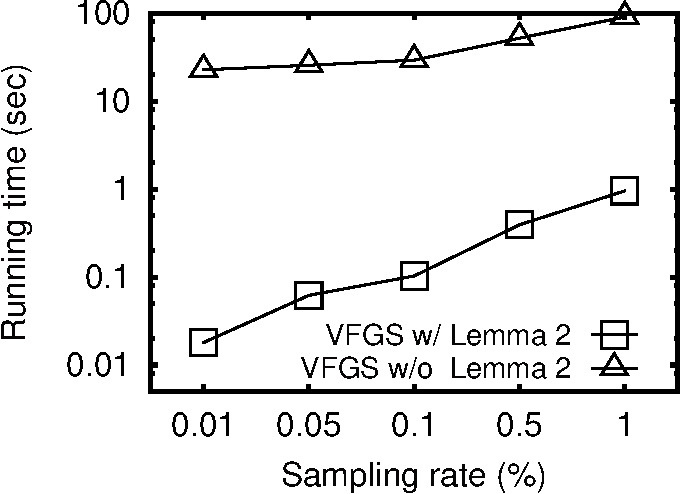
\includegraphics[width=0.44\columnwidth]{pictures/tshenzhen}
%		\\
%		(A) \pt{}
%		&
%		(B) \sz{}	
%	\end{tabular}
%	\vspace{-3mm}
%	\caption{Running time of $\vats$ w/ and w/o Lemma~\ref{lem:submodular}.}
%	\label{fig:cost}
%	\vspace{-6mm}
%\end{figure}
%\QM{unfininshed}
%We first conduct an experiment to evaluate the rendering cost by datasize. We vary the number of trajectories from 1000 to 1 million, which are randomly selected from \pt{} dataset. The experimental results are summarized in Table~\ref{tab:gpu}. We observe that the rendering cost is linear with the input data trajectories.
%
%We first report the running time of our $\vats$ algorithm in Figure~\ref{fig:cost} by varying the sampling rate from $0.01\%$ to $1\%$. The results show that $\vats$ is quite slow without the submodularity of contribution value, which agrees with Lemma~\ref{lem:submodular} in Section~\ref{sec:opt}.
%Then we shown the total time usage with sampling rate as Figure~\ref{fig:sample_time}. {*******}
%
%The optimized $\vats$ (e.g., $\vats$ with Lemma~\ref{lem:submodular}) outperforms $\vats$ by one to three orders of magnitudes on both datasets. The result show that running time of our $\vats$ algorithm is below 1 second in most cases. We have shown that $\vats$ provides good visualization performance with a low sampling rate (e.g., $0.1\%$ or $1\%$) in Section 6.1 and 6.2,  and Table~\ref{tab:gpu} suggests that the rendering latency scales almost linearly with dataset cardinality. By significantly reducing the dataset cardinality with sampling, $\vats$ can effectively reduces the rendering latency to make interactive visualization possible without sacrificing visual quality. For example, rendering the full $\pt{}$ dataset takes about \QM{34 seconds}, with a sampling rate of $1\%$, $\vats$ can bring down the rendering latency to less than 1 second.





\section{Conclusions}\label{sec:con}
%Visualizing large trajectory dataset is challenge due to two reasons: visual clutter and long rendering time.
%Data sampling technique, an effective method in reducing the rendering time by shrinking the data size, has been applied in a variety of data.
%However, very few work target at the trajectory sampling especially from the perspective of visualization.
%The most commonly used sampling method, uniform random sampling technique, always generate results with very poor visual quality because very few trajectories located at margin regions can be preserved.
%We fill the gap by proposing a novel sampling techniques $\avats$ which guarantees the visual quality at overview and reduce the visual clutter at the detail view. The technique characteristics and a series of parameters setting are discussed.
%We compare $\avats$ with uniform random sampling in regarding to visual quality preservation and time-usage. We evaluate the effectiveness of proposed method by applying our method to different dataset and conducting users studies on specific interactive trajectory exploration tasks.
%Even though it is recommended to use our method with caching techniques, our experience in the experiment shows that a faster algorithm will be more user friendly for the real world ad-hoc exploration tasks. For future work, we first plan to reduce the time usage by leveraging the advanced database techniques such as the indexing technique or use GPU acceleration.
%In addition, there are several directions can be further explored to enrich the information presented by the visualization.
%First we will develop different color encoding schema to present the spatial distribution of trajectory more precisely.
%In current schema, the color of one trajectory is the same, thus the color of the long trajectories may mislead the users because they pass  through many regions with different level of the traffic crowdedness. One solution is to use gradient color schema to encode the trajectories.
%Another interesting direction is to extend the approach to support the mulit-class characteristics which is a commonly existed in variety of trajectory dataset.


This paper presents the $\avats$ framework, which achieves high visual quality and low visualization latency for large-scale trajectory datasets. $\avats$ provides guaranteed visual quality in trajectory sampling by formulating a quality optimal sampling problem and developing effective solutions including $\vats$ and $\vats$. Low visualization latency is achieved with the $\invQ$-tree index, which allows to use the sampling results computed offline. Experiment results show that $\avats$ consistently provides high quality visualization in different cases and its visualization time is orders of magnitude shorter than full visualization.
%We plan to extend $\avats$ to support the specific trajectory features such as mulit-class characteristics in the future. 

%a novel sampling technique, $\avats$, that guarantees the visual quality of line-based trajectory visualization and alleviates the visual clutter problem. The effectiveness and efficiency of the proposed method are validated with real world visual analysis tasks and quantitatively performance measurements. Possible future directions include (i) improving visual quality by sampling trajectory segments instead of complete trajectories and (ii) developing advanced color encoding schemes to better describe the spatial distribution of the trajectories.
%extending our approaches to support the specific trajectory features such as mulit-class characteristics.

%we focus on the sampling approach of trajectory segments other than the whole trajectories to achieve higher visual fidelity.
%We will also develop different color encoding schema to present the spatial distribution of trajectories more precisely. Currently, the color of one trajectory keep the same, thus the color of the long trajectories may mislead the users because they may pass through many regions with different traffic crowdedness.
%We also consider to extend our approach to support the specific trajectory features such as mulit-class characteristics. 


%\IEEEraisesectionheading{\section{Introduction}\label{sec:introduction}}
% Computer Society journal (but not conference!) papers do something unusual
% with the very first section heading (almost always called "Introduction").
% They place it ABOVE the main text! IEEEtran.cls does not automatically do
% this for you, but you can achieve this effect with the provided
% \IEEEraisesectionheading{} command. Note the need to keep any \label that
% is to refer to the section immediately after \section in the above as
% \IEEEraisesectionheading puts \section within a raised box.




% The very first letter is a 2 line initial drop letter followed
% by the rest of the first word in caps (small caps for compsoc).
% 
% form to use if the first word consists of a single letter:
% \IEEEPARstart{A}{demo} file is ....
% 
% form to use if you need the single drop letter followed by
% normal text (unknown if ever used by the IEEE):
% \IEEEPARstart{A}{}demo file is ....
% 
% Some journals put the first two words in caps:
% \IEEEPARstart{T}{his demo} file is ....
% 
% Here we have the typical use of a "T" for an initial drop letter
% and "HIS" in caps to complete the first word.

%\subsection{Subsection Heading Here}
%Subsection text here.

% needed in second column of first page if using \IEEEpubid
%\IEEEpubidadjcol

%\subsubsection{Subsubsection Heading Here}
%Subsubsection text here.


% An example of a floating figure using the graphicx package.
% Note that \label must occur AFTER (or within) \caption.
% For figures, \caption should occur after the \includegraphics.
% Note that IEEEtran v1.7 and later has special internal code that
% is designed to preserve the operation of \label within \caption
% even when the captionsoff option is in effect. However, because
% of issues like this, it may be the safest practice to put all your
% \label just after \caption rather than within \caption{}.
%
% Reminder: the "draftcls" or "draftclsnofoot", not "draft", class
% option should be used if it is desired that the figures are to be
% displayed while in draft mode.
%
%\begin{figure}[!t]
%\centering
%\includegraphics[width=2.5in]{myfigure}
% where an .eps filename suffix will be assumed under latex, 
% and a .pdf suffix will be assumed for pdflatex; or what has been declared
% via \DeclareGraphicsExtensions.
%\caption{Simulation results for the network.}
%\label{fig_sim}
%\end{figure}

% Note that the IEEE typically puts floats only at the top, even when this
% results in a large percentage of a column being occupied by floats.
% However, the Computer Society has been known to put floats at the bottom.


% An example of a double column floating figure using two subfigures.
% (The subfig.sty package must be loaded for this to work.)
% The subfigure \label commands are set within each subfloat command,
% and the \label for the overall figure must come after \caption.
% \hfil is used as a separator to get equal spacing.
% Watch out that the combined width of all the subfigures on a 
% line do not exceed the text width or a line break will occur.
%
%\begin{figure*}[!t]
%\centering
%\subfloat[Case I]{\includegraphics[width=2.5in]{box}%
%\label{fig_first_case}}
%\hfil
%\subfloat[Case II]{\includegraphics[width=2.5in]{box}%
%\label{fig_second_case}}
%\caption{Simulation results for the network.}
%\label{fig_sim}
%\end{figure*}
%
% Note that often IEEE papers with subfigures do not employ subfigure
% captions (using the optional argument to \subfloat[]), but instead will
% reference/describe all of them (a), (b), etc., within the main caption.
% Be aware that for subfig.sty to generate the (a), (b), etc., subfigure
% labels, the optional argument to \subfloat must be present. If a
% subcaption is not desired, just leave its contents blank,
% e.g., \subfloat[].


% An example of a floating table. Note that, for IEEE style tables, the
% \caption command should come BEFORE the table and, given that table
% captions serve much like titles, are usually capitalized except for words
% such as a, an, and, as, at, but, by, for, in, nor, of, on, or, the, to
% and up, which are usually not capitalized unless they are the first or
% last word of the caption. Table text will default to \footnotesize as
% the IEEE normally uses this smaller font for tables.
% The \label must come after \caption as always.
%
%\begin{table}[!t]
%% increase table row spacing, adjust to taste
%\renewcommand{\arraystretch}{1.3}
% if using array.sty, it might be a good idea to tweak the value of
% \extrarowheight as needed to properly center the text within the cells
%\caption{An Example of a Table}
%\label{table_example}
%\centering
%% Some packages, such as MDW tools, offer better commands for making tables
%% than the plain LaTeX2e tabular which is used here.
%\begin{tabular}{|c||c|}
%\hline
%One & Two\\
%\hline
%Three & Four\\
%\hline
%\end{tabular}
%\end{table}


% Note that the IEEE does not put floats in the very first column
% - or typically anywhere on the first page for that matter. Also,
% in-text middle ("here") positioning is typically not used, but it
% is allowed and encouraged for Computer Society conferences (but
% not Computer Society journals). Most IEEE journals/conferences use
% top floats exclusively. 
% Note that, LaTeX2e, unlike IEEE journals/conferences, places
% footnotes above bottom floats. This can be corrected via the
% \fnbelowfloat command of the stfloats package.








% if have a single appendix:
%\appendix[Proof of the Zonklar Equations]
% or
%\appendix  % for no appendix heading
% do not use \section anymore after \appendix, only \section*
% is possibly needed

% use appendices with more than one appendix
% then use \section to start each appendix
% you must declare a \section before using any
% \subsection or using \label (\appendices by itself
% starts a section numbered zero.)
%





% use section* for acknowledgment
\ifCLASSOPTIONcompsoc
  % The Computer Society usually uses the plural form
  \section*{Acknowledgments}
\else
  % regular IEEE prefers the singular form
  \section*{Acknowledgment}
\fi


The authors would like to thank...


% Can use something like this to put references on a page
% by themselves when using endfloat and the captionsoff option.
\ifCLASSOPTIONcaptionsoff
  \newpage
\fi



% trigger a \newpage just before the given reference
% number - used to balance the columns on the last page
% adjust value as needed - may need to be readjusted if
% the document is modified later
%\IEEEtriggeratref{8}
% The "triggered" command can be changed if desired:
%\IEEEtriggercmd{\enlargethispage{-5in}}

% references section

% can use a bibliography generated by BibTeX as a .bbl file
% BibTeX documentation can be easily obtained at:
% http://mirror.ctan.org/biblio/bibtex/contrib/doc/
% The IEEEtran BibTeX style support page is at:
% http://www.michaelshell.org/tex/ieeetran/bibtex/
\bibliographystyle{IEEEtran}
% argument is your BibTeX string definitions and bibliography database(s)
\bibliography{ref}
%
% <OR> manually copy in the resultant .bbl file
% set second argument of \begin to the number of references
% (used to reserve space for the reference number labels box)


% biography section
% 
% If you have an EPS/PDF photo (graphicx package needed) extra braces are
% needed around the contents of the optional argument to biography to prevent
% the LaTeX parser from getting confused when it sees the complicated
% \includegraphics command within an optional argument. (You could create
% your own custom macro containing the \includegraphics command to make things
% simpler here.)
%\begin{IEEEbiography}[{\includegraphics[width=1in,height=1.25in,clip,keepaspectratio]{mshell}}]{Michael Shell}
% or if you just want to reserve a space for a photo:

\begin{IEEEbiography}{Michael Shell}
Biography text here.
\end{IEEEbiography}

% if you will not have a photo at all:
\begin{IEEEbiographynophoto}{John Doe}
Biography text here.
\end{IEEEbiographynophoto}

% insert where needed to balance the two columns on the last page with
% biographies
%\newpage

\begin{IEEEbiographynophoto}{Jane Doe}
Biography text here.
\end{IEEEbiographynophoto}

% You can push biographies down or up by placing
% a \vfill before or after them. The appropriate
% use of \vfill depends on what kind of text is
% on the last page and whether or not the columns
% are being equalized.

%\vfill

% Can be used to pull up biographies so that the bottom of the last one
% is flush with the other column.
%\enlargethispage{-5in}



% that's all folks

\end{document}


